%%%%%%%%%%%%%%%%%%%%%%%%%%%%%%%%%%%%%%%%%%%%%%%%%%%%%%%%%%%%%%%%%%%%%%%%%%%%%%%%
% Preámbulo                                                                    %
%%%%%%%%%%%%%%%%%%%%%%%%%%%%%%%%%%%%%%%%%%%%%%%%%%%%%%%%%%%%%%%%%%%%%%%%%%%%%%%%

\documentclass[11pt,a4paper,titlepage,twoside,openright,openbib,spanish]{report}

%%% RELACIÓN DE VARIABLES A PERSONALIZAR %%%
\def\lingua{esp} % descomenta esta liña se redactarás a memoria en español
\def\nome{Alonso Rodriguez Iglesias}                             % substitúe aquí o teu nome
\def\nomedirectorA{Juan Touriño Domínguez}             % substitúe aquí o nome de quen dirixe
\def\nomedirectorB{María José Martín Santamaría}             % substitúe aquí o nome de quen dirixe
\def\titulo{Diseño e implementación hardware y software de un mini-supercomputador con Raspberry Pi} % substitúe aquí o título do teu TFG
\def\mencion{ENXEÑARÍA DE COMPUTADORES}

\def\renomearcadros{si} % descomenta esta liña se redactas a memoria en español e prefires que
                         % os "cuadros" e o "índice de cuadros" se renomeen
                         % a "tablas" e "índice de tablas" respectivamente

\usepackage{estilo_tfg}

% Lista de paquetes potencialmente interesantes (uso baixo demanda)

\usepackage[all]{nowidow}
% \usepackage{alltt}       % proporciona o entorno alltt, semellante a verbatim pero que respecta comandos
% \usepackage{enumitem}    % permite personalizar os entornos de lista
% \usepackage{eurofont}    % proporciona o comando \euro
\usepackage{eurosym}
\usepackage{float}       % permite máis opcións para controlar obxectos flotantes (táboas, figuras)
\usepackage{hhline}      % permie personalizar as liñas horizontais en arrays e táboas
% \usepackage{longtable}   % permite construir táboas que ocupan máis dunha páxina
\usepackage{lscape}      % permite colocar partes do documento en orientación apaisada
% \usepackage{moreverb}    % permite personalizar o entorno verbatim
\usepackage{multirow}    % permite crear celdas que ocupan varias filas da mesma táboa
\usepackage{pdfpages}    % permite insertar ficheiros en PDF no documento
\usepackage{rotating}    % permite diferentes tipos de rotacións para figuras e táboas
% \usepackage{subcaption}  % permite a inclusión de varias subfiguras nunha figura
% \usepackage{tabu}        % permite táboas flexibles
% \usepackage{tabularx}    % permite táboas con columnas de anchura determinada
\usepackage{pdflscape}
\usepackage{translator}
\usepackage{placeins}
\usepackage{tablefootnote}

\usepackage[scale=MatchLowercase]{sourcecodepro}
\usepackage{pgfplots}
\usepackage{pgfgantt}
\newganttlinktype{F-S}{
  \ganttsetstartanchor{east}
  \ganttsetendanchor{west}
  \draw [/pgfgantt/link] (\xLeft - 0.2,\yUpper) -- (\xRight + 0.2, \yLower);
}

\newganttlinktype{F_S}{
  \ganttsetstartanchor{east}
  \ganttsetendanchor{west}
  \draw [/pgfgantt/link] (\xLeft - 0.2,\yUpper) |- (\xRight + 0.2, \yLower);
}

\newganttlinktype{S-S}{
  \ganttsetstartanchor{west}
  \ganttsetendanchor{west}
  \draw [/pgfgantt/link] (\xLeft + 0.2,\yUpper) |- (\xRight, \yLower);
}

\newganttlinktype{F-F}{
  \ganttsetstartanchor{east}
  \ganttsetendanchor{east}
  \draw [/pgfgantt/link] (\xLeft - 0.2 ,\yUpper) -| (\xRight - 0.2, \yLower);
}

\newganttlinktype{F-S}{
  \ganttsetstartanchor{east}
  \ganttsetendanchor{west}
  \draw [/pgfgantt/link] (\xLeft - 0.2,\yUpper) -| (\xRight + 0.2, \yLower);
}
\usepackage{pgfplotstable}
\pgfplotsset{compat = newest}
\usepackage{wrapfig}
\usepackage{etoolbox}
\BeforeBeginEnvironment{wrapfigure}{\setlength{\intextsep}{0pt}}
\usepackage{svg}
\usepackage{adjustbox}
\newcommand{\vasymptote}[2][]{
    \draw [thick,ficblue,densely dashed,#1] ({rel axis cs:0,0} -| {axis cs:#2,0}) -- ({rel axis cs:0,1} -| {axis cs:#2,0});
}
\pgfplotsset{every axis/.append style={
        scaled y ticks = false, 
        scaled x ticks = false, 
        y tick label style={/pgf/number format/.cd, fixed},
        x tick label style={/pgf/number format/.cd, fixed}
    }
}

%%%%%%%%%%%%%%%%%%%%%%%%%%%%%%%%%%%%%%%%%%%%%%%%%%%%%%%%%%%%%%%%%%%%%%%%%%%%%%%%
% Corpo                                                                        %
%%%%%%%%%%%%%%%%%%%%%%%%%%%%%%%%%%%%%%%%%%%%%%%%%%%%%%%%%%%%%%%%%%%%%%%%%%%%%%%%

\begin{document}

%%%%%%%%%%%%%%%%%%%%%%%%%%%%%%%%%%%%%%%%
% Preliminares do documento            %
%%%%%%%%%%%%%%%%%%%%%%%%%%%%%%%%%%%%%%%%

\begin{titlepage}
  
  \hspace*{128pt}
  \textcolor{udcpink}{{\fontencoding{T1}\fontfamily{phv}\selectfont Facultade de Informática}}\\[-32pt]

  \begin{center}
    
\includegraphics[scale=0.3]{imaxes/udc}\\[35pt]

    {\large TRABALLO FIN DE GRAO \\
            GRAO EN ENXEÑARÍA INFORMÁTICA \\
            MENCIÓN EN \mencion } \\[100pt]
    
    \begin{huge}
      \begin{spacing}{1.3}
        \bfseries \titulo
      \end{spacing}
    \end{huge}
  \end{center}
  
  \vfill
  
  \begin{flushright}
    {\large
    \begin{tabular}{ll}
      {\bf Estudante:} & \nome \\
      {\bf Dirección:} & \nomedirectorA \\ % COPIA E PEGA ESTA LIÑA MÁIS VECES SE O PRECISAS
      {\bf Dirección:} & \nomedirectorB \\ % COPIA E PEGA ESTA LIÑA MÁIS VECES SE O PRECISAS
    \end{tabular}}
  \end{flushright}
  \rightline{A Coruña, \today.}
\end{titlepage}

\paxinaenbranco
\begin{flushright}
\dedicatoria{A todas las personas que me apoyaron en los buenos y los malos momentos.\\Gracias a ellos hoy soy quien soy.}
\end{flushright}
\paxinaenbranco
\paxinaenbranco
\begin{agradecementos}
A todas las personas que me han acompañado a lo largo de mi vida, en especial a mi familia y amigos, por estar ahí cuando se los necesitaba, por los buenos momentos que hemos pasado juntos, y su permanente e incondicional apoyo.

A todas las increíbles personas que he conocido y con las que he tenido el placer de compartir prácticas y tiempo juntos. Ellos saben quienes son.

A todos los profesores con los que he disfrutado aprendiendo, por muy difícil que fuese la materia, y que permiten que nuevas generaciones sigan explorando este apasionante mundo de la ingeniería informática. En especial a mis tutores Juan y María José, por depositar su confianza en mí, guiarme por el camino correcto, y por su inestimable trabajo y ayuda.

Muchas gracias.

\begin{flushright}
Alonso
\end{flushright}
\end{agradecementos}
% Ugly hack to fix random pagenumber %%%%%%
\pagenumbering{gobble}
\pagestyle{empty}
%%%%%%%%%%%%%%%%%%%%%%%%%%%%%%%%%%%%%%%%%%%
\paxinaenbranco
%%%%%%%%%%%%%%%%%%%%%%%%%%%%%%%%%%%%%%%%%%%%%%%%%%%%%%%%%%%%%%%%%%%%%%%%%%%%%%%%

\begin{abstract}\thispagestyle{empty}
  \blindtext % substitúe este comando polo resumo do teu TFG
             % na lingua principal do documento (tipicamente: galego)

  \vspace*{25pt}
  \begin{segundoresumo}
    \blindtext % substitúe este comando polo resumo do teu TFG
               % na lingua secundaria do documento (tipicamente: inglés)
  \end{segundoresumo}
\vspace*{25pt}
\begin{multicols}{2}
\begin{description}
\item [\palabraschaveprincipal:] \mbox{} \\[-20pt]
  \blindlist{itemize}[7] % substitúe este comando por un itemize
                         % que relacione as palabras chave
                         % que mellor identifiquen o teu TFG
                         % no idioma principal da memoria (tipicamente: galego)
\end{description}
\begin{description}
\item [\palabraschavesecundaria:] \mbox{} \\[-20pt]
  \blindlist{itemize}[7] % substitúe este comando por un itemize
                         % que relacione as palabras chave
                         % que mellor identifiquen o teu TFG
                         % no idioma secundario da memoria (tipicamente: inglés)
\end{description}
\end{multicols}

\end{abstract}

%%%%%%%%%%%%%%%%%%%%%%%%%%%%%%%%%%%%%%%%%%%%%%%%%%%%%%%%%%%%%%%%%%%%%%%%%%%%%%%%

%\paxinaenbranco
%Restore thinges %%%
\pagestyle{fancy}
%%%%%%%%%%%%%%%%%%%%

\pagenumbering{roman}
\setcounter{page}{1}
\bstctlcite{IEEEexample:BSTcontrol}

\tableofcontents
\listoffigures
\listoftables
\cleardoublepage

\pagenumbering{arabic}
\setcounter{page}{1}

%%%%%%%%%%%%%%%%%%%%%%%%%%%%%%%%%%%%%%%%
% Capítulos                            %
%%%%%%%%%%%%%%%%%%%%%%%%%%%%%%%%%%%%%%%%

\chapter{Introdución}
\label{chap:introducion}

\lettrine{P}{rimer} capítulo da memoria, onde xeralmente se exporán as
liñas mestras do traballo, os obxectivos, etc. Incluimos un par de
exemplos de citas~\cite{ErlangBook,ErlangWebBook} e de referencias
internas (sección \ref{sec:mostra}, páxina \pageref{sec:mostra}).

\Blindtext

\section{Sección de mostra}
\label{sec:mostra}

\Blindtext

\subsection{Subsección de mostra}

\Blindtext

\chapter{Clúpiter: Conceptos básicos}
\label{chap:conceptos_basicos}

\lettrine{P}{ara} comprender el objetivo del proyecto y su propuesta de valor, primero es necesario entender sus características, la justificación de las mismas, y el funcionamiento de sus componentes más primitivos.

\section{Nombre y marca corporativa}
Si bien este no es un elemento altamente importante en un proyecto de ingeniería como este, si que es conveniente, y nunca está de más, otorgarle personalidad mediante la creación de un nombre e isotipo para el mismo.

El nombre del clúster es \textbf{Clúpiter} (ClúPIter): una mezcla entre las palabras ``Clúster'' y el ``PI'' de la \acrlong{rpi}, que de forma muy conveniente recuerda en su segunda parte a Júpiter. Este es a su vez planeta del sistema solar junto con el (enano) Plutón, nombre del clúster del \acrshort{gac}\footnote{\url{http://pluton.dec.udc.es}} (\acrlong{gac}). Es cuanto menos paradógico que el clúster en miniatura sea Júpiter, y el real sea Plutón\dots

En cuanto a la marca del clúster, éste no puede quedar sin un logo, que se muestra en la Figura \ref{fig:clupiter_logo}.\footnote{El uso del logo de Arch Linux sin autorización explícita está permitido en general para propósitos no comerciales. Clúpiter no tiene ningún tipo de vinculación con la marca Arch Linux (\url{https://wiki.archlinux.org/title/DeveloperWiki:TrademarkPolicy})}

\begin{figure}[h!]
  \centering
  \vspace*{0.5cm}
  \def\svgwidth{0.50\textwidth}
  \input{pdf_tex/clupiter_logo/clupiter_logo.pdf_tex}
  \caption{Logo de Clúpiter}
  \label{fig:clupiter_logo}
\end{figure}

\section{Clústeres}
Los clústeres, de los que para este proyecto se tratarán los de alto rendimiento, son conjuntos de ordenadores diseñados para ofrecer altas prestaciones de cálculo.

Estos clústeres pueden ser homogéneos o heterogéneos, siendo compuestos por computadores con la misma arquitectura y capacidades, o con arquitecturas o capacidades diferentes, respectivamente.

En el caso de Clúpiter, éste es un clúster muy homogéneo, ya que está compuesto por ocho mini-computadores exactamente iguales.

Existen multitud de amateurs y amantes de la informática que como proyecto personal deciden montar un clúster de \acrlong{rpi}s, entre los que por ejemplo se encuentra Jeff Geerling\footnote{\url{https://www.youtube.com/user/geerlingguy}}, un famoso YouTuber del cual uno de sus proyectos se puede encontrar en la Figura \ref{fig:cluster-pi-ejemplo}.

\begin{figure}[h!]
  \centering
  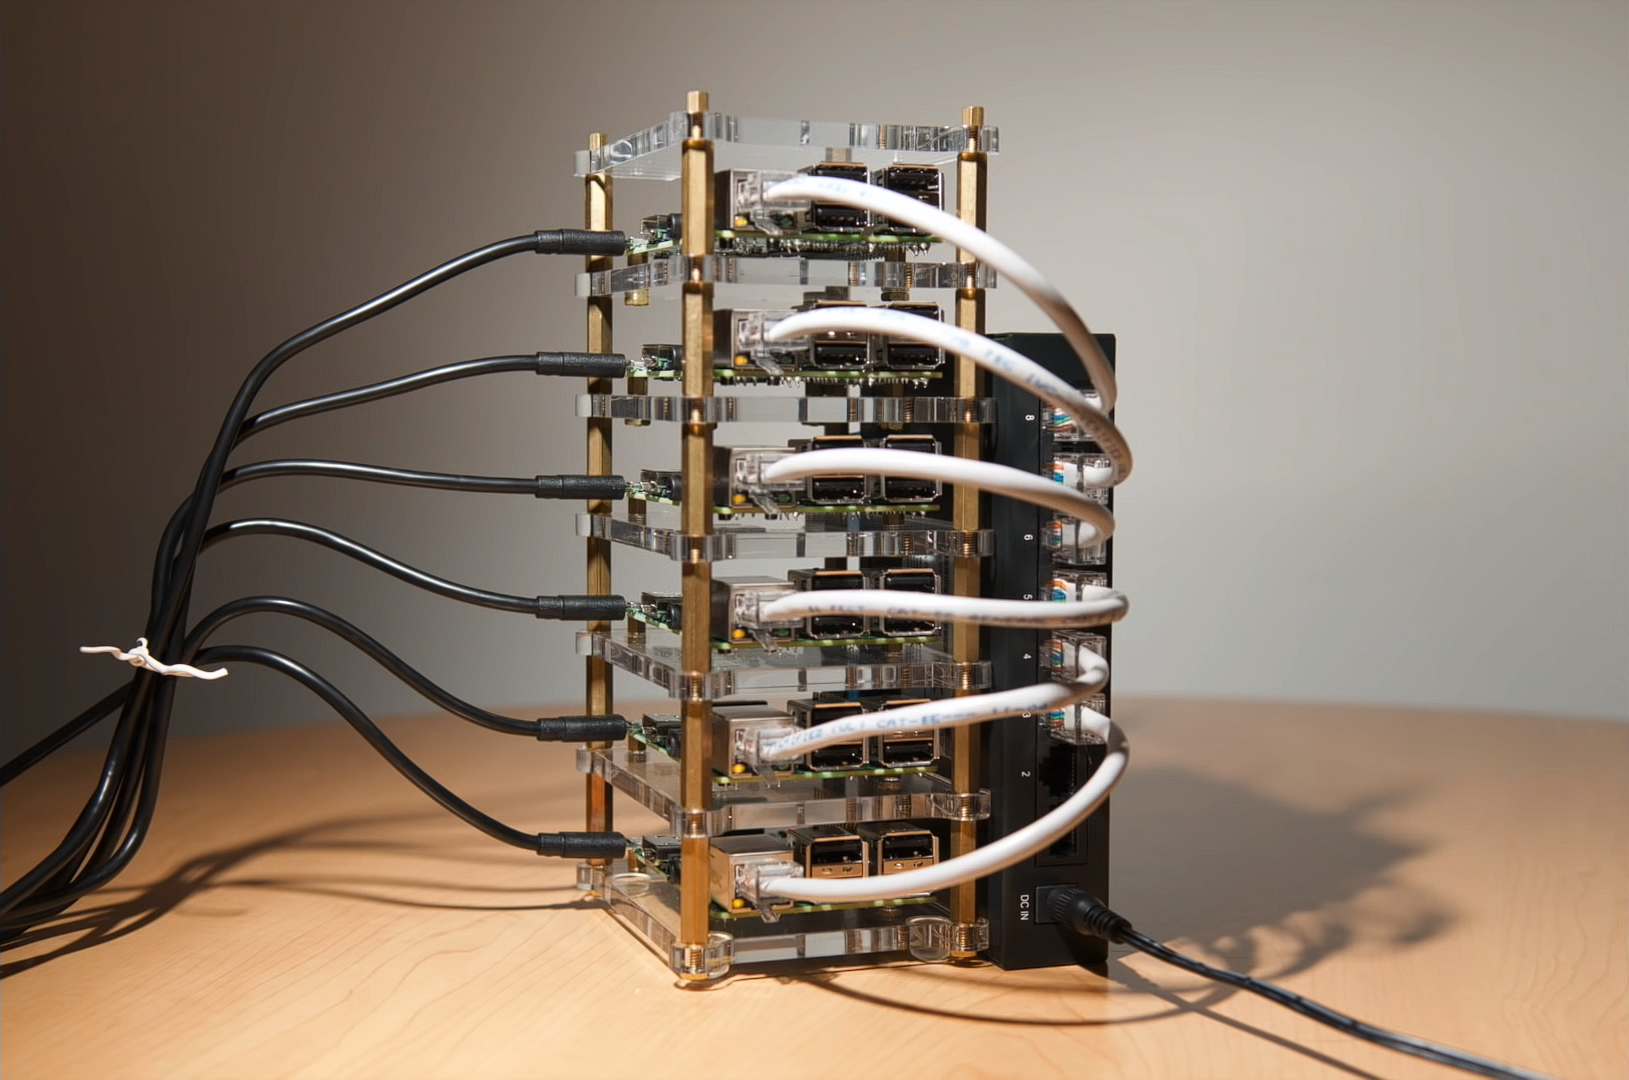
\includegraphics[width=0.75\textwidth]{img/cluster-pi-home.png}
  \caption{Mini-clúster casero basado en \acrlong{rpi} 3\cite{geerling_intro_cluster}}
  \label{fig:cluster-pi-ejemplo}
\end{figure}

Además, en el mundo académico también ha habido aproximaciones similares al trabajo desarrollado, destacando \textit{Wee Archie}, un clúster de 18 \acrlong{rpi} 2 que, como se puede leer en la página web del proyecto \cite{wee_archie_webpage}, pretende emular el comportamiento de un supercomputador real, el supercomputador ARCHER\footnote{\url{https://www.archer.ac.uk}} (Figura \ref{fig:wee_archie_girl}).

\begin{figure}[h!]
  \centering
  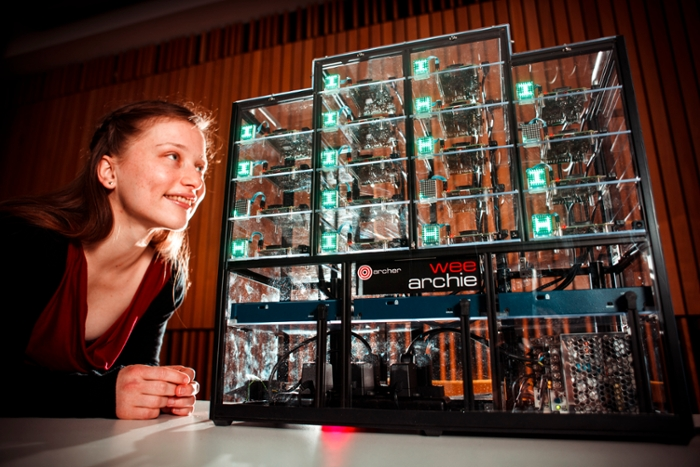
\includegraphics[width=0.75\textwidth]{img/wee-girl.jpg}
  \caption{Mini-supercomputador Wee Archie}
  \label{fig:wee_archie_girl}
\end{figure}

\section{Raspberry Pi 4 Model B}
\label{sec:raspberry_pi_4_model_b}
Cada aproximadamente dos años, la Raspberry Pi Foundation saca una nueva versión de su compacto y más exitoso producto: la \acrlong{rpi}, o por sus siglas \acrshort{rpi}. Estos pequeños computadores vienen en diversos formatos de forma, pero el que ha catapultado esta plataforma al éxito ha sido el formato que denominan \textit{Standard}\footnote{85.6 mm × 56.5 mm}.

\begin{figure}[h!]
  \centering
  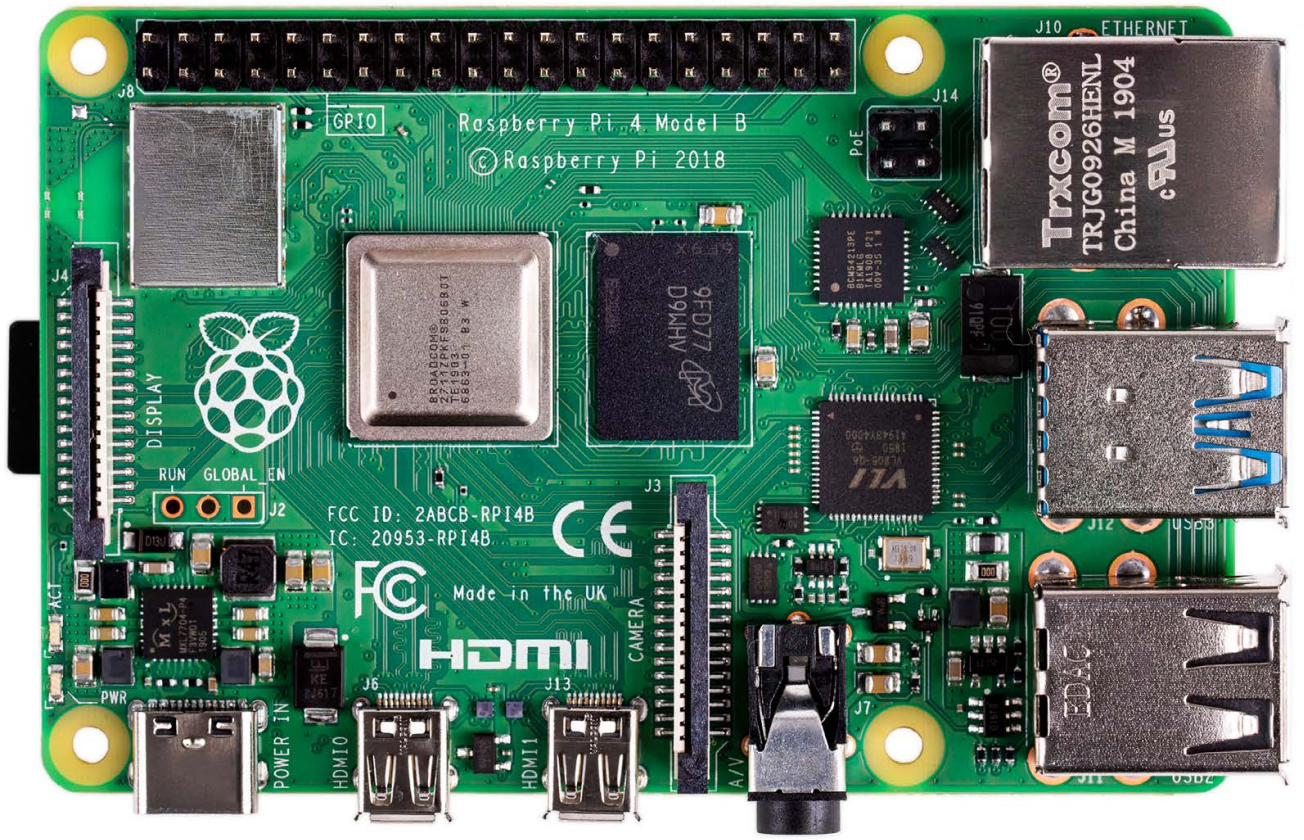
\includegraphics[width=0.75\textwidth]{img/rpi_parts/rpi_base.jpg}
  \caption{\acrlong{rpi} 4 Model B}
  \label{fig:rpi_base}
\end{figure}

Siendo cada versión mucho más potente que la anterior, y costando aproximadamente el mismo precio, está claro que la Raspberry Pi Foundation está haciendo un excelente trabajo aportando valor a este segmento del bajo consumo y coste.

La \acrlong{rpi} 4B (4 Model B), que se muestra en la Figura \ref{fig:rpi_base}, es la versión más nueva de formato \textit{Standard}, y por ello ha sido la elección para constituir la base del clúster. A continuación se muestran sus principales características \cite{rpi4b_specifications}:

\subsection{CPU}
La \acrshort{cpu} (\textit{\acrlong{cpu}} o Unidad de Procesamiento Central) de este nuevo modelo es la \textbf{Broadcom BCM2711}, un procesador con arquitectura ARMv8-A y 4 núcleos Cortex-A72, que funcionan a 1.5GHz.

Estos núcleos cuentan con un \textit{pipeline} de 15 etapas, ejecución OOO (\textit{out-of-order}) y predictor de saltos, entre otros.

Además, cuenta con 48KB de L1I y 32KB de L1D por núcleo, así como 1MB de L2 compartido (256KB por núcleo). Esto emparejado con un único chip de 2GB de memoria LPDDR4-3200, es suficiente para un uso doméstico sencillo, pero quizás no sea la mejor disposición para el cómputo intensivo como se verá más adelante.
% TODO INSERTAR REF?????

\subsection{GPU/VPU}
\label{ssec:gpu_vpu}
A pesar de que el integrado que se muestra en la foto del apartado superior es un \acrshort{soc} (\textit{\acrlong{soc}}), se ha preferido tratar la \acrshort{cpu} y la \acrshort{gpu}/\acrshort{vpu} (\textit{\acrlong{gpu}}/\textit{\acrlong{vpu}}) por separado. Y es que los gráficos integrados de esta última \acrlong{rpi} son una importante mejora sobre la VideoCore IV que equipaban modelos anteriores.

La GPU en la \acrshort{rpi}4 es la VideoCore VI, y cuenta con multitud de soporte para multimedia y una potencia gráfica aceptable. En concreto, acelera por hardware H.265 (4Kp60 decode), H.264 (1080p60 decode, 1080p30 encode), y soporta OpenGL ES, 3.0.

Además, y lo que considero más interesante, es que posteriormente al lanzamiento se comenzó para esta gráfica el desarrollo de un driver de Vulkan: un estándar abierto de última generación para programación de gráficos, pero que también se puede emplear para cómputo. Esto es una fantástica noticia, ya que permite acelerar ciertas cargas de trabajo aprovechando la inmensa capacidad de cómputo paralelo de estos dispositivos, siendo una de las más habituales en estos dispositivos la transformada de Fourier.

Realizar algún tipo de programa para computación \acrshort{gpgpu} (\textit{\acrlong{gpgpu}}) en Vulkan queda fuera de lo que pretende abarcar este trabajo, pero es un interesante proyecto para la realización de alguna otra iteración sobre esta plataforma.

\subsection{E/S}
En términos de \acrlong{e-s} (\acrshort{e-s}) la \acrshort{rpi}4B cuenta con multitud de puertos, de los que se van a utilizar Gigabit Ethernet y USB 3.0. Sin embargo, éste equipa de serie otros muchos otros puertos en los pines \acrshort{gpio} (\acrlong{gpio}), cuya disposición se puede encontrar en la Figura \ref{fig:rpi_gpio_pinout}, y que es un estándar de-facto, ya que es la misma para todos los modelos de \acrlong{rpi} y otros dispositivos similares, que la adoptan para mayor inter-compatibilidad.

Los puertos y protocolos que integra la \acrlong{rpi} en el \acrshort{gpio} son algunos como I2C (\textit{Inter-Integrated Circuit}), UART (\textit{Universal Asynchronous Receiver-Transmitter}), SPI (\textit{Serial Peripheral Interface}) y video compuesto, así como mútiples pines de alimentación a 5 y 3.3V. Por último, ya en la propia placa, tambien se dispone de un puerto DSI (\textit{Display Serial Interface}) y CSI (\textit{Camera Serial Interface}), y dos salidas de vídeo HDMI.

También cuenta con interfaz de datos inalámbrica, que soporta tecnologías WiFi 802.11.b/g/n/ac y Bluetooth 5.0.

\begin{figure}[h!]
  \centering
  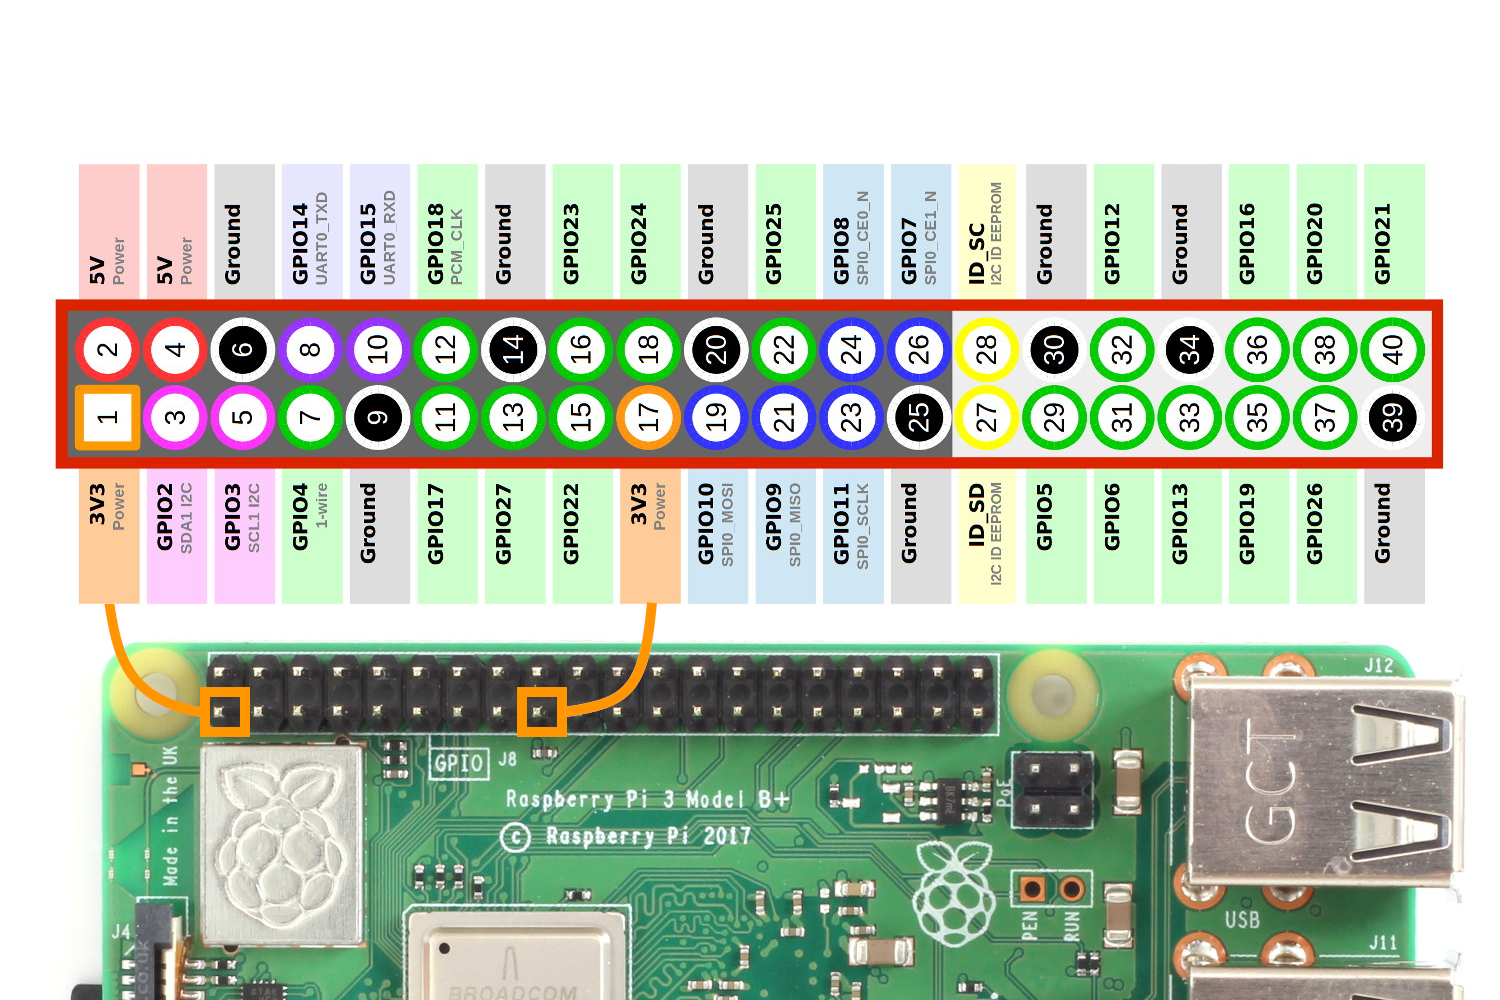
\includegraphics[width=0.85\textwidth]{img/rpi_parts/rpi_gpio.png}
  \caption{Pines GPIO de la \acrlong{rpi} 4}
  \label{fig:rpi_gpio_pinout}
\end{figure}

\section{MPI}
Para aprovechar todo el potencial hardware de los supercomputadores y, en general, de los computadores paralelos, existen paradigmas de programación específicos. \acrshort{mpi} (\acrlong{mpi})\footnote{\url{https://www.mpi-forum.org}} es un estándar para la programación de los sistemas paralelos de memoria distribuida como Clúpiter. Es una especificación de paso de mensajes que define la sintaxis y semántica del conjunto de rutinas para comunicar datos entre procesos que exponen las diferentes implementaciones. 

Entre las implementaciones disponibles, las más utilizadas son:
\begin{itemize}
  \item\textbf{OpenMPI}\footnote{\url{https://www.open-mpi.org}}: Implementación libre mantenida por un consorcio de académicos, investigadores y socios que ofrece elevada eficiencia y flexibilidad a quien la implementa. Además, es la librería \acrshort{mpi} que ofrece Arch Linux (distribución Linux de Clúpiter) en sus repositorios oficiales, y contra la que se compilan por defecto sus ejecutables.
  \item\textbf{MPICH}\footnote{\url{https://www.mpich.org}}: Otra implementación libre de MPI muy similar a OpenMPI en rendimiento, flexibilidad y modo de desarrollo.
  \item\textbf{Intel MPI}\footnote{\url{https://software.intel.com/content/www/us/en/develop/tools/oneapi/components/mpi-library.html}}: Implementación propietaria de \acrshort{mpi} por parte de Intel. Está especializada en productos de la propia marca y optimizaza para ellos, por lo que suele arrojar un mayor rendimiento que las contrapartes libres.
\end{itemize}

La base de \acrshort{mpi} son las primitivas de envío y recepción de datos. Existen dos funciones de envío y recepción \textbf{síncronas} (esto es, la llamada a la función solamente termina cuando todos los miembros involucrados en la ejecución de dicha función han terminado):
\begin{itemize}
  \item \textbf{MPI\_Send}: Envía un mensaje a destino, y espera a que el receptor esté listo para recibirlo. 
  \item \textbf{MPI\_Recv}: Espera a que llegue un mensaje del origen, y cuando éste está listo para enviarlo, lo recibe.
\end{itemize}

Estas funciones tienen su contraparte para programación asíncrona, que puede arrojar un mayor rendimiento, pero también requiere un extra de complejidad y puede no ser trivial. Las funciones básicas para realizar programación asíncrona con \acrshort{mpi} son \textbf{MPI\_Isend} y \textbf{MPI\_Irecv}. A su vez son necesarias para chequear el estado de la ejecución asíncrona las funciones \textbf{MPI\_Test} (asíncrona) y \textbf{MPI\_Wait} (síncrona).

Otra funcionalidad de \acrshort{mpi} ampliamente utilizada son las primitivas de grupo u operaciones colectivas, las cuales permiten la comunicación entre más de 2 procesos.

Las colectivas más sencillas y comunes de MPI son las siguientes \cite{cheung_mpi}:
\begin{itemize}
  \item \textbf{MPI\_Bcast}: Emite (hace \textit{broadcast}) el mensaje a todos los procesos del comunicador, tal y como se muestra en la Figura \ref{fig:mpi_bcast}.
  
  \begin{figure}[H]
    \vspace*{0.5cm}
    \centering
    \resizebox {0.8\textwidth} {!} {
    % Created by Eps2pgf 0.7.0 (build on 2008-08-24) on Sun Aug 22 14:08:15 CEST 2021
\begin{pgfpicture}
\pgfpathmoveto{\pgfqpoint{0cm}{0cm}}
\pgfpathlineto{\pgfqpoint{25.188cm}{0cm}}
\pgfpathlineto{\pgfqpoint{25.188cm}{10.724cm}}
\pgfpathlineto{\pgfqpoint{0cm}{10.724cm}}
\pgfpathclose
\pgfusepath{clip}
\begin{pgfscope}
\pgfpathmoveto{\pgfqpoint{0cm}{10.724cm}}
\pgfpathlineto{\pgfqpoint{0cm}{0cm}}
\pgfpathlineto{\pgfqpoint{25.188cm}{0cm}}
\pgfpathlineto{\pgfqpoint{25.188cm}{10.724cm}}
\pgfpathclose
\pgfusepath{clip}
\begin{pgfscope}
\begin{pgfscope}
\definecolor{eps2pgf_color}{rgb}{1,1,0}\pgfsetstrokecolor{eps2pgf_color}\pgfsetfillcolor{eps2pgf_color}
\pgfpathmoveto{\pgfqpoint{5.429cm}{5.92cm}}
\pgfpathlineto{\pgfqpoint{17.97cm}{5.92cm}}
\pgfpathlineto{\pgfqpoint{17.97cm}{4.173cm}}
\pgfpathlineto{\pgfqpoint{5.429cm}{4.173cm}}
\pgfpathclose
\pgfseteorule\pgfusepath{fill}\pgfsetnonzerorule
\end{pgfscope}
\begin{pgfscope}
\pgfsetdash{}{0cm}
\pgfsetlinewidth{0.317mm}
\definecolor{eps2pgf_color}{rgb}{1,1,0}\pgfsetstrokecolor{eps2pgf_color}\pgfsetfillcolor{eps2pgf_color}
\pgfpathmoveto{\pgfqpoint{5.429cm}{5.92cm}}
\pgfpathlineto{\pgfqpoint{17.97cm}{5.92cm}}
\pgfpathlineto{\pgfqpoint{17.97cm}{4.173cm}}
\pgfpathlineto{\pgfqpoint{5.429cm}{4.173cm}}
\pgfpathclose
\pgfusepath{stroke}
\end{pgfscope}
\begin{pgfscope}
\definecolor{eps2pgf_color}{rgb}{0.53,0.81,1}\pgfsetstrokecolor{eps2pgf_color}\pgfsetfillcolor{eps2pgf_color}
\pgfpathmoveto{\pgfqpoint{2.73cm}{9.095cm}}
\pgfpathlineto{\pgfqpoint{3.524cm}{9.095cm}}
\pgfpathlineto{\pgfqpoint{3.524cm}{8.301cm}}
\pgfpathlineto{\pgfqpoint{2.73cm}{8.301cm}}
\pgfpathclose
\pgfseteorule\pgfusepath{fill}\pgfsetnonzerorule
\end{pgfscope}
\begin{pgfscope}
\pgfsetdash{}{0cm}
\pgfsetlinewidth{0.317mm}
\definecolor{eps2pgf_color}{gray}{0}\pgfsetstrokecolor{eps2pgf_color}\pgfsetfillcolor{eps2pgf_color}
\pgfpathmoveto{\pgfqpoint{2.73cm}{9.095cm}}
\pgfpathlineto{\pgfqpoint{3.524cm}{9.095cm}}
\pgfpathlineto{\pgfqpoint{3.524cm}{8.301cm}}
\pgfpathlineto{\pgfqpoint{2.73cm}{8.301cm}}
\pgfpathclose
\pgfusepath{stroke}
\end{pgfscope}
\begin{pgfscope}
\definecolor{eps2pgf_color}{rgb}{0,1,0}\pgfsetstrokecolor{eps2pgf_color}\pgfsetfillcolor{eps2pgf_color}
\pgfpathmoveto{\pgfqpoint{3.524cm}{9.095cm}}
\pgfpathlineto{\pgfqpoint{4.318cm}{9.095cm}}
\pgfpathlineto{\pgfqpoint{4.318cm}{8.301cm}}
\pgfpathlineto{\pgfqpoint{3.524cm}{8.301cm}}
\pgfpathclose
\pgfseteorule\pgfusepath{fill}\pgfsetnonzerorule
\end{pgfscope}
\begin{pgfscope}
\pgfsetdash{}{0cm}
\pgfsetlinewidth{0.317mm}
\definecolor{eps2pgf_color}{gray}{0}\pgfsetstrokecolor{eps2pgf_color}\pgfsetfillcolor{eps2pgf_color}
\pgfpathmoveto{\pgfqpoint{3.524cm}{9.095cm}}
\pgfpathlineto{\pgfqpoint{4.318cm}{9.095cm}}
\pgfpathlineto{\pgfqpoint{4.318cm}{8.301cm}}
\pgfpathlineto{\pgfqpoint{3.524cm}{8.301cm}}
\pgfpathclose
\pgfusepath{stroke}
\end{pgfscope}
\begin{pgfscope}
\definecolor{eps2pgf_color}{rgb}{1,1,0}\pgfsetstrokecolor{eps2pgf_color}\pgfsetfillcolor{eps2pgf_color}
\pgfpathmoveto{\pgfqpoint{1.937cm}{9.095cm}}
\pgfpathlineto{\pgfqpoint{2.73cm}{9.095cm}}
\pgfpathlineto{\pgfqpoint{2.73cm}{8.301cm}}
\pgfpathlineto{\pgfqpoint{1.937cm}{8.301cm}}
\pgfpathclose
\pgfseteorule\pgfusepath{fill}\pgfsetnonzerorule
\end{pgfscope}
\begin{pgfscope}
\pgfsetdash{}{0cm}
\pgfsetlinewidth{0.317mm}
\definecolor{eps2pgf_color}{gray}{0}\pgfsetstrokecolor{eps2pgf_color}\pgfsetfillcolor{eps2pgf_color}
\pgfpathmoveto{\pgfqpoint{1.937cm}{9.095cm}}
\pgfpathlineto{\pgfqpoint{2.73cm}{9.095cm}}
\pgfpathlineto{\pgfqpoint{2.73cm}{8.301cm}}
\pgfpathlineto{\pgfqpoint{1.937cm}{8.301cm}}
\pgfpathclose
\pgfusepath{stroke}
\end{pgfscope}
\begin{pgfscope}
\definecolor{eps2pgf_color}{rgb}{1,0.75,0.75}\pgfsetstrokecolor{eps2pgf_color}\pgfsetfillcolor{eps2pgf_color}
\pgfpathmoveto{\pgfqpoint{4.318cm}{9.095cm}}
\pgfpathlineto{\pgfqpoint{5.112cm}{9.095cm}}
\pgfpathlineto{\pgfqpoint{5.112cm}{8.301cm}}
\pgfpathlineto{\pgfqpoint{4.318cm}{8.301cm}}
\pgfpathclose
\pgfseteorule\pgfusepath{fill}\pgfsetnonzerorule
\end{pgfscope}
\begin{pgfscope}
\pgfsetdash{}{0cm}
\pgfsetlinewidth{0.317mm}
\definecolor{eps2pgf_color}{gray}{0}\pgfsetstrokecolor{eps2pgf_color}\pgfsetfillcolor{eps2pgf_color}
\pgfpathmoveto{\pgfqpoint{4.318cm}{9.095cm}}
\pgfpathlineto{\pgfqpoint{5.112cm}{9.095cm}}
\pgfpathlineto{\pgfqpoint{5.112cm}{8.301cm}}
\pgfpathlineto{\pgfqpoint{4.318cm}{8.301cm}}
\pgfpathclose
\pgfusepath{stroke}
\end{pgfscope}
\begin{pgfscope}
\definecolor{eps2pgf_color}{rgb}{0.53,0.81,1}\pgfsetstrokecolor{eps2pgf_color}\pgfsetfillcolor{eps2pgf_color}
\pgfpathmoveto{\pgfqpoint{2.889cm}{1.157cm}}
\pgfpathlineto{\pgfqpoint{3.683cm}{1.157cm}}
\pgfpathlineto{\pgfqpoint{3.683cm}{0.363cm}}
\pgfpathlineto{\pgfqpoint{2.889cm}{0.363cm}}
\pgfpathclose
\pgfseteorule\pgfusepath{fill}\pgfsetnonzerorule
\end{pgfscope}
\begin{pgfscope}
\pgfsetdash{}{0cm}
\pgfsetlinewidth{0.317mm}
\definecolor{eps2pgf_color}{gray}{0}\pgfsetstrokecolor{eps2pgf_color}\pgfsetfillcolor{eps2pgf_color}
\pgfpathmoveto{\pgfqpoint{2.889cm}{1.157cm}}
\pgfpathlineto{\pgfqpoint{3.683cm}{1.157cm}}
\pgfpathlineto{\pgfqpoint{3.683cm}{0.363cm}}
\pgfpathlineto{\pgfqpoint{2.889cm}{0.363cm}}
\pgfpathclose
\pgfusepath{stroke}
\end{pgfscope}
\begin{pgfscope}
\definecolor{eps2pgf_color}{rgb}{0,1,0}\pgfsetstrokecolor{eps2pgf_color}\pgfsetfillcolor{eps2pgf_color}
\pgfpathmoveto{\pgfqpoint{3.683cm}{1.157cm}}
\pgfpathlineto{\pgfqpoint{4.477cm}{1.157cm}}
\pgfpathlineto{\pgfqpoint{4.477cm}{0.363cm}}
\pgfpathlineto{\pgfqpoint{3.683cm}{0.363cm}}
\pgfpathclose
\pgfseteorule\pgfusepath{fill}\pgfsetnonzerorule
\end{pgfscope}
\begin{pgfscope}
\pgfsetdash{}{0cm}
\pgfsetlinewidth{0.317mm}
\definecolor{eps2pgf_color}{gray}{0}\pgfsetstrokecolor{eps2pgf_color}\pgfsetfillcolor{eps2pgf_color}
\pgfpathmoveto{\pgfqpoint{3.683cm}{1.157cm}}
\pgfpathlineto{\pgfqpoint{4.477cm}{1.157cm}}
\pgfpathlineto{\pgfqpoint{4.477cm}{0.363cm}}
\pgfpathlineto{\pgfqpoint{3.683cm}{0.363cm}}
\pgfpathclose
\pgfusepath{stroke}
\end{pgfscope}
\begin{pgfscope}
\definecolor{eps2pgf_color}{rgb}{1,1,0}\pgfsetstrokecolor{eps2pgf_color}\pgfsetfillcolor{eps2pgf_color}
\pgfpathmoveto{\pgfqpoint{2.095cm}{1.157cm}}
\pgfpathlineto{\pgfqpoint{2.889cm}{1.157cm}}
\pgfpathlineto{\pgfqpoint{2.889cm}{0.363cm}}
\pgfpathlineto{\pgfqpoint{2.095cm}{0.363cm}}
\pgfpathclose
\pgfseteorule\pgfusepath{fill}\pgfsetnonzerorule
\end{pgfscope}
\begin{pgfscope}
\pgfsetdash{}{0cm}
\pgfsetlinewidth{0.317mm}
\definecolor{eps2pgf_color}{gray}{0}\pgfsetstrokecolor{eps2pgf_color}\pgfsetfillcolor{eps2pgf_color}
\pgfpathmoveto{\pgfqpoint{2.095cm}{1.157cm}}
\pgfpathlineto{\pgfqpoint{2.889cm}{1.157cm}}
\pgfpathlineto{\pgfqpoint{2.889cm}{0.363cm}}
\pgfpathlineto{\pgfqpoint{2.095cm}{0.363cm}}
\pgfpathclose
\pgfusepath{stroke}
\end{pgfscope}
\begin{pgfscope}
\definecolor{eps2pgf_color}{rgb}{1,0.75,0.75}\pgfsetstrokecolor{eps2pgf_color}\pgfsetfillcolor{eps2pgf_color}
\pgfpathmoveto{\pgfqpoint{4.477cm}{1.157cm}}
\pgfpathlineto{\pgfqpoint{5.27cm}{1.157cm}}
\pgfpathlineto{\pgfqpoint{5.27cm}{0.363cm}}
\pgfpathlineto{\pgfqpoint{4.477cm}{0.363cm}}
\pgfpathclose
\pgfseteorule\pgfusepath{fill}\pgfsetnonzerorule
\end{pgfscope}
\begin{pgfscope}
\pgfsetdash{}{0cm}
\pgfsetlinewidth{0.317mm}
\definecolor{eps2pgf_color}{gray}{0}\pgfsetstrokecolor{eps2pgf_color}\pgfsetfillcolor{eps2pgf_color}
\pgfpathmoveto{\pgfqpoint{4.477cm}{1.157cm}}
\pgfpathlineto{\pgfqpoint{5.27cm}{1.157cm}}
\pgfpathlineto{\pgfqpoint{5.27cm}{0.363cm}}
\pgfpathlineto{\pgfqpoint{4.477cm}{0.363cm}}
\pgfpathclose
\pgfusepath{stroke}
\end{pgfscope}
\begin{pgfscope}
\definecolor{eps2pgf_color}{rgb}{0.53,0.81,1}\pgfsetstrokecolor{eps2pgf_color}\pgfsetfillcolor{eps2pgf_color}
\pgfpathmoveto{\pgfqpoint{9.557cm}{1.316cm}}
\pgfpathlineto{\pgfqpoint{10.35cm}{1.316cm}}
\pgfpathlineto{\pgfqpoint{10.35cm}{0.522cm}}
\pgfpathlineto{\pgfqpoint{9.557cm}{0.522cm}}
\pgfpathclose
\pgfseteorule\pgfusepath{fill}\pgfsetnonzerorule
\end{pgfscope}
\begin{pgfscope}
\pgfsetdash{}{0cm}
\pgfsetlinewidth{0.317mm}
\definecolor{eps2pgf_color}{gray}{0}\pgfsetstrokecolor{eps2pgf_color}\pgfsetfillcolor{eps2pgf_color}
\pgfpathmoveto{\pgfqpoint{9.557cm}{1.316cm}}
\pgfpathlineto{\pgfqpoint{10.35cm}{1.316cm}}
\pgfpathlineto{\pgfqpoint{10.35cm}{0.522cm}}
\pgfpathlineto{\pgfqpoint{9.557cm}{0.522cm}}
\pgfpathclose
\pgfusepath{stroke}
\end{pgfscope}
\begin{pgfscope}
\definecolor{eps2pgf_color}{rgb}{0,1,0}\pgfsetstrokecolor{eps2pgf_color}\pgfsetfillcolor{eps2pgf_color}
\pgfpathmoveto{\pgfqpoint{10.35cm}{1.316cm}}
\pgfpathlineto{\pgfqpoint{11.144cm}{1.316cm}}
\pgfpathlineto{\pgfqpoint{11.144cm}{0.522cm}}
\pgfpathlineto{\pgfqpoint{10.35cm}{0.522cm}}
\pgfpathclose
\pgfseteorule\pgfusepath{fill}\pgfsetnonzerorule
\end{pgfscope}
\begin{pgfscope}
\pgfsetdash{}{0cm}
\pgfsetlinewidth{0.317mm}
\definecolor{eps2pgf_color}{gray}{0}\pgfsetstrokecolor{eps2pgf_color}\pgfsetfillcolor{eps2pgf_color}
\pgfpathmoveto{\pgfqpoint{10.35cm}{1.316cm}}
\pgfpathlineto{\pgfqpoint{11.144cm}{1.316cm}}
\pgfpathlineto{\pgfqpoint{11.144cm}{0.522cm}}
\pgfpathlineto{\pgfqpoint{10.35cm}{0.522cm}}
\pgfpathclose
\pgfusepath{stroke}
\end{pgfscope}
\begin{pgfscope}
\definecolor{eps2pgf_color}{rgb}{1,1,0}\pgfsetstrokecolor{eps2pgf_color}\pgfsetfillcolor{eps2pgf_color}
\pgfpathmoveto{\pgfqpoint{8.763cm}{1.316cm}}
\pgfpathlineto{\pgfqpoint{9.557cm}{1.316cm}}
\pgfpathlineto{\pgfqpoint{9.557cm}{0.522cm}}
\pgfpathlineto{\pgfqpoint{8.763cm}{0.522cm}}
\pgfpathclose
\pgfseteorule\pgfusepath{fill}\pgfsetnonzerorule
\end{pgfscope}
\begin{pgfscope}
\pgfsetdash{}{0cm}
\pgfsetlinewidth{0.317mm}
\definecolor{eps2pgf_color}{gray}{0}\pgfsetstrokecolor{eps2pgf_color}\pgfsetfillcolor{eps2pgf_color}
\pgfpathmoveto{\pgfqpoint{8.763cm}{1.316cm}}
\pgfpathlineto{\pgfqpoint{9.557cm}{1.316cm}}
\pgfpathlineto{\pgfqpoint{9.557cm}{0.522cm}}
\pgfpathlineto{\pgfqpoint{8.763cm}{0.522cm}}
\pgfpathclose
\pgfusepath{stroke}
\end{pgfscope}
\begin{pgfscope}
\definecolor{eps2pgf_color}{rgb}{1,0.75,0.75}\pgfsetstrokecolor{eps2pgf_color}\pgfsetfillcolor{eps2pgf_color}
\pgfpathmoveto{\pgfqpoint{11.144cm}{1.316cm}}
\pgfpathlineto{\pgfqpoint{11.938cm}{1.316cm}}
\pgfpathlineto{\pgfqpoint{11.938cm}{0.522cm}}
\pgfpathlineto{\pgfqpoint{11.144cm}{0.522cm}}
\pgfpathclose
\pgfseteorule\pgfusepath{fill}\pgfsetnonzerorule
\end{pgfscope}
\begin{pgfscope}
\pgfsetdash{}{0cm}
\pgfsetlinewidth{0.317mm}
\definecolor{eps2pgf_color}{gray}{0}\pgfsetstrokecolor{eps2pgf_color}\pgfsetfillcolor{eps2pgf_color}
\pgfpathmoveto{\pgfqpoint{11.144cm}{1.316cm}}
\pgfpathlineto{\pgfqpoint{11.938cm}{1.316cm}}
\pgfpathlineto{\pgfqpoint{11.938cm}{0.522cm}}
\pgfpathlineto{\pgfqpoint{11.144cm}{0.522cm}}
\pgfpathclose
\pgfusepath{stroke}
\end{pgfscope}
\begin{pgfscope}
\definecolor{eps2pgf_color}{rgb}{0.53,0.81,1}\pgfsetstrokecolor{eps2pgf_color}\pgfsetfillcolor{eps2pgf_color}
\pgfpathmoveto{\pgfqpoint{15.907cm}{1.316cm}}
\pgfpathlineto{\pgfqpoint{16.7cm}{1.316cm}}
\pgfpathlineto{\pgfqpoint{16.7cm}{0.522cm}}
\pgfpathlineto{\pgfqpoint{15.907cm}{0.522cm}}
\pgfpathclose
\pgfseteorule\pgfusepath{fill}\pgfsetnonzerorule
\end{pgfscope}
\begin{pgfscope}
\pgfsetdash{}{0cm}
\pgfsetlinewidth{0.317mm}
\definecolor{eps2pgf_color}{gray}{0}\pgfsetstrokecolor{eps2pgf_color}\pgfsetfillcolor{eps2pgf_color}
\pgfpathmoveto{\pgfqpoint{15.907cm}{1.316cm}}
\pgfpathlineto{\pgfqpoint{16.7cm}{1.316cm}}
\pgfpathlineto{\pgfqpoint{16.7cm}{0.522cm}}
\pgfpathlineto{\pgfqpoint{15.907cm}{0.522cm}}
\pgfpathclose
\pgfusepath{stroke}
\end{pgfscope}
\begin{pgfscope}
\definecolor{eps2pgf_color}{rgb}{0,1,0}\pgfsetstrokecolor{eps2pgf_color}\pgfsetfillcolor{eps2pgf_color}
\pgfpathmoveto{\pgfqpoint{16.7cm}{1.316cm}}
\pgfpathlineto{\pgfqpoint{17.494cm}{1.316cm}}
\pgfpathlineto{\pgfqpoint{17.494cm}{0.522cm}}
\pgfpathlineto{\pgfqpoint{16.7cm}{0.522cm}}
\pgfpathclose
\pgfseteorule\pgfusepath{fill}\pgfsetnonzerorule
\end{pgfscope}
\begin{pgfscope}
\pgfsetdash{}{0cm}
\pgfsetlinewidth{0.317mm}
\definecolor{eps2pgf_color}{gray}{0}\pgfsetstrokecolor{eps2pgf_color}\pgfsetfillcolor{eps2pgf_color}
\pgfpathmoveto{\pgfqpoint{16.7cm}{1.316cm}}
\pgfpathlineto{\pgfqpoint{17.494cm}{1.316cm}}
\pgfpathlineto{\pgfqpoint{17.494cm}{0.522cm}}
\pgfpathlineto{\pgfqpoint{16.7cm}{0.522cm}}
\pgfpathclose
\pgfusepath{stroke}
\end{pgfscope}
\begin{pgfscope}
\definecolor{eps2pgf_color}{rgb}{1,1,0}\pgfsetstrokecolor{eps2pgf_color}\pgfsetfillcolor{eps2pgf_color}
\pgfpathmoveto{\pgfqpoint{15.113cm}{1.316cm}}
\pgfpathlineto{\pgfqpoint{15.907cm}{1.316cm}}
\pgfpathlineto{\pgfqpoint{15.907cm}{0.522cm}}
\pgfpathlineto{\pgfqpoint{15.113cm}{0.522cm}}
\pgfpathclose
\pgfseteorule\pgfusepath{fill}\pgfsetnonzerorule
\end{pgfscope}
\begin{pgfscope}
\pgfsetdash{}{0cm}
\pgfsetlinewidth{0.317mm}
\definecolor{eps2pgf_color}{gray}{0}\pgfsetstrokecolor{eps2pgf_color}\pgfsetfillcolor{eps2pgf_color}
\pgfpathmoveto{\pgfqpoint{15.113cm}{1.316cm}}
\pgfpathlineto{\pgfqpoint{15.907cm}{1.316cm}}
\pgfpathlineto{\pgfqpoint{15.907cm}{0.522cm}}
\pgfpathlineto{\pgfqpoint{15.113cm}{0.522cm}}
\pgfpathclose
\pgfusepath{stroke}
\end{pgfscope}
\begin{pgfscope}
\definecolor{eps2pgf_color}{rgb}{1,0.75,0.75}\pgfsetstrokecolor{eps2pgf_color}\pgfsetfillcolor{eps2pgf_color}
\pgfpathmoveto{\pgfqpoint{17.494cm}{1.316cm}}
\pgfpathlineto{\pgfqpoint{18.288cm}{1.316cm}}
\pgfpathlineto{\pgfqpoint{18.288cm}{0.522cm}}
\pgfpathlineto{\pgfqpoint{17.494cm}{0.522cm}}
\pgfpathclose
\pgfseteorule\pgfusepath{fill}\pgfsetnonzerorule
\end{pgfscope}
\begin{pgfscope}
\pgfsetdash{}{0cm}
\pgfsetlinewidth{0.317mm}
\definecolor{eps2pgf_color}{gray}{0}\pgfsetstrokecolor{eps2pgf_color}\pgfsetfillcolor{eps2pgf_color}
\pgfpathmoveto{\pgfqpoint{17.494cm}{1.316cm}}
\pgfpathlineto{\pgfqpoint{18.288cm}{1.316cm}}
\pgfpathlineto{\pgfqpoint{18.288cm}{0.522cm}}
\pgfpathlineto{\pgfqpoint{17.494cm}{0.522cm}}
\pgfpathclose
\pgfusepath{stroke}
\end{pgfscope}
\begin{pgfscope}
\definecolor{eps2pgf_color}{rgb}{0.53,0.81,1}\pgfsetstrokecolor{eps2pgf_color}\pgfsetfillcolor{eps2pgf_color}
\pgfpathmoveto{\pgfqpoint{22.415cm}{1.475cm}}
\pgfpathlineto{\pgfqpoint{23.209cm}{1.475cm}}
\pgfpathlineto{\pgfqpoint{23.209cm}{0.681cm}}
\pgfpathlineto{\pgfqpoint{22.415cm}{0.681cm}}
\pgfpathclose
\pgfseteorule\pgfusepath{fill}\pgfsetnonzerorule
\end{pgfscope}
\begin{pgfscope}
\pgfsetdash{}{0cm}
\pgfsetlinewidth{0.317mm}
\definecolor{eps2pgf_color}{gray}{0}\pgfsetstrokecolor{eps2pgf_color}\pgfsetfillcolor{eps2pgf_color}
\pgfpathmoveto{\pgfqpoint{22.415cm}{1.475cm}}
\pgfpathlineto{\pgfqpoint{23.209cm}{1.475cm}}
\pgfpathlineto{\pgfqpoint{23.209cm}{0.681cm}}
\pgfpathlineto{\pgfqpoint{22.415cm}{0.681cm}}
\pgfpathclose
\pgfusepath{stroke}
\end{pgfscope}
\begin{pgfscope}
\definecolor{eps2pgf_color}{rgb}{0,1,0}\pgfsetstrokecolor{eps2pgf_color}\pgfsetfillcolor{eps2pgf_color}
\pgfpathmoveto{\pgfqpoint{23.209cm}{1.475cm}}
\pgfpathlineto{\pgfqpoint{24.003cm}{1.475cm}}
\pgfpathlineto{\pgfqpoint{24.003cm}{0.681cm}}
\pgfpathlineto{\pgfqpoint{23.209cm}{0.681cm}}
\pgfpathclose
\pgfseteorule\pgfusepath{fill}\pgfsetnonzerorule
\end{pgfscope}
\begin{pgfscope}
\pgfsetdash{}{0cm}
\pgfsetlinewidth{0.317mm}
\definecolor{eps2pgf_color}{gray}{0}\pgfsetstrokecolor{eps2pgf_color}\pgfsetfillcolor{eps2pgf_color}
\pgfpathmoveto{\pgfqpoint{23.209cm}{1.475cm}}
\pgfpathlineto{\pgfqpoint{24.003cm}{1.475cm}}
\pgfpathlineto{\pgfqpoint{24.003cm}{0.681cm}}
\pgfpathlineto{\pgfqpoint{23.209cm}{0.681cm}}
\pgfpathclose
\pgfusepath{stroke}
\end{pgfscope}
\begin{pgfscope}
\definecolor{eps2pgf_color}{rgb}{1,1,0}\pgfsetstrokecolor{eps2pgf_color}\pgfsetfillcolor{eps2pgf_color}
\pgfpathmoveto{\pgfqpoint{21.622cm}{1.475cm}}
\pgfpathlineto{\pgfqpoint{22.415cm}{1.475cm}}
\pgfpathlineto{\pgfqpoint{22.415cm}{0.681cm}}
\pgfpathlineto{\pgfqpoint{21.622cm}{0.681cm}}
\pgfpathclose
\pgfseteorule\pgfusepath{fill}\pgfsetnonzerorule
\end{pgfscope}
\begin{pgfscope}
\pgfsetdash{}{0cm}
\pgfsetlinewidth{0.317mm}
\definecolor{eps2pgf_color}{gray}{0}\pgfsetstrokecolor{eps2pgf_color}\pgfsetfillcolor{eps2pgf_color}
\pgfpathmoveto{\pgfqpoint{21.622cm}{1.475cm}}
\pgfpathlineto{\pgfqpoint{22.415cm}{1.475cm}}
\pgfpathlineto{\pgfqpoint{22.415cm}{0.681cm}}
\pgfpathlineto{\pgfqpoint{21.622cm}{0.681cm}}
\pgfpathclose
\pgfusepath{stroke}
\end{pgfscope}
\begin{pgfscope}
\definecolor{eps2pgf_color}{rgb}{1,0.75,0.75}\pgfsetstrokecolor{eps2pgf_color}\pgfsetfillcolor{eps2pgf_color}
\pgfpathmoveto{\pgfqpoint{24.003cm}{1.475cm}}
\pgfpathlineto{\pgfqpoint{24.797cm}{1.475cm}}
\pgfpathlineto{\pgfqpoint{24.797cm}{0.681cm}}
\pgfpathlineto{\pgfqpoint{24.003cm}{0.681cm}}
\pgfpathclose
\pgfseteorule\pgfusepath{fill}\pgfsetnonzerorule
\end{pgfscope}
\begin{pgfscope}
\pgfsetdash{}{0cm}
\pgfsetlinewidth{0.317mm}
\definecolor{eps2pgf_color}{gray}{0}\pgfsetstrokecolor{eps2pgf_color}\pgfsetfillcolor{eps2pgf_color}
\pgfpathmoveto{\pgfqpoint{24.003cm}{1.475cm}}
\pgfpathlineto{\pgfqpoint{24.797cm}{1.475cm}}
\pgfpathlineto{\pgfqpoint{24.797cm}{0.681cm}}
\pgfpathlineto{\pgfqpoint{24.003cm}{0.681cm}}
\pgfpathclose
\pgfusepath{stroke}
\end{pgfscope}
\begin{pgfscope}
\definecolor{eps2pgf_color}{gray}{0}\pgfsetstrokecolor{eps2pgf_color}\pgfsetfillcolor{eps2pgf_color}
\pgftext[x=3.183cm,y=10.369cm,rotate=0]{\fontsize{27.1}{32.52}\selectfont{\textrm{\textbf{P}}}}
\end{pgfscope}
\begin{pgfscope}
\definecolor{eps2pgf_color}{gray}{0}\pgfsetstrokecolor{eps2pgf_color}\pgfsetfillcolor{eps2pgf_color}
\pgftext[x=3.556cm,y=9.987cm,rotate=0]{\fontsize{21.68}{26.02}\selectfont{\textrm{\textbf{0}}}}
\end{pgfscope}
\begin{pgfscope}
\definecolor{eps2pgf_color}{gray}{0}\pgfsetstrokecolor{eps2pgf_color}\pgfsetfillcolor{eps2pgf_color}
\pgftext[x=9.85cm,y=10.369cm,rotate=0]{\fontsize{27.1}{32.52}\selectfont{\textrm{\textbf{P}}}}
\end{pgfscope}
\begin{pgfscope}
\definecolor{eps2pgf_color}{gray}{0}\pgfsetstrokecolor{eps2pgf_color}\pgfsetfillcolor{eps2pgf_color}
\pgftext[x=10.226cm,y=10.15cm,rotate=0]{\fontsize{21.68}{26.02}\selectfont{\textrm{\textbf{1}}}}
\end{pgfscope}
\begin{pgfscope}
\definecolor{eps2pgf_color}{gray}{0}\pgfsetstrokecolor{eps2pgf_color}\pgfsetfillcolor{eps2pgf_color}
\pgftext[x=16.2cm,y=10.369cm,rotate=0]{\fontsize{27.1}{32.52}\selectfont{\textrm{\textbf{P}}}}
\end{pgfscope}
\begin{pgfscope}
\definecolor{eps2pgf_color}{gray}{0}\pgfsetstrokecolor{eps2pgf_color}\pgfsetfillcolor{eps2pgf_color}
\pgftext[x=16.572cm,y=9.992cm,rotate=0]{\fontsize{21.68}{26.02}\selectfont{\textrm{\textbf{2}}}}
\end{pgfscope}
\begin{pgfscope}
\definecolor{eps2pgf_color}{gray}{0}\pgfsetstrokecolor{eps2pgf_color}\pgfsetfillcolor{eps2pgf_color}
\pgftext[x=22.55cm,y=10.21cm,rotate=0]{\fontsize{27.1}{32.52}\selectfont{\textrm{\textbf{P}}}}
\end{pgfscope}
\begin{pgfscope}
\definecolor{eps2pgf_color}{gray}{0}\pgfsetstrokecolor{eps2pgf_color}\pgfsetfillcolor{eps2pgf_color}
\pgftext[x=22.917cm,y=9.986cm,rotate=0]{\fontsize{21.68}{26.02}\selectfont{\textrm{\textbf{3}}}}
\end{pgfscope}
\begin{pgfscope}
\pgfsetdash{}{0cm}
\pgfsetlinewidth{0.317mm}
\definecolor{eps2pgf_color}{gray}{0}\pgfsetstrokecolor{eps2pgf_color}\pgfsetfillcolor{eps2pgf_color}
\pgfpathmoveto{\pgfqpoint{1.619cm}{9.412cm}}
\pgfpathlineto{\pgfqpoint{5.429cm}{9.412cm}}
\pgfpathlineto{\pgfqpoint{5.429cm}{7.983cm}}
\pgfpathlineto{\pgfqpoint{1.619cm}{7.983cm}}
\pgfpathclose
\pgfusepath{stroke}
\end{pgfscope}
\begin{pgfscope}
\definecolor{eps2pgf_color}{gray}{0}\pgfsetstrokecolor{eps2pgf_color}\pgfsetfillcolor{eps2pgf_color}
\pgftext[x=0.74cm,y=9.489cm,rotate=0]{\fontsize{27.1}{32.52}\selectfont{\textrm{\textbf{\textit{buf}}}}}
\end{pgfscope}
\begin{pgfscope}
\pgfsetdash{}{0cm}
\pgfsetlinewidth{0.317mm}
\definecolor{eps2pgf_color}{gray}{0}\pgfsetstrokecolor{eps2pgf_color}\pgfsetfillcolor{eps2pgf_color}
\pgfpathmoveto{\pgfqpoint{1.778cm}{1.475cm}}
\pgfpathlineto{\pgfqpoint{5.588cm}{1.475cm}}
\pgfpathlineto{\pgfqpoint{5.588cm}{0.046cm}}
\pgfpathlineto{\pgfqpoint{1.778cm}{0.046cm}}
\pgfpathclose
\pgfusepath{stroke}
\end{pgfscope}
\begin{pgfscope}
\definecolor{eps2pgf_color}{gray}{0}\pgfsetstrokecolor{eps2pgf_color}\pgfsetfillcolor{eps2pgf_color}
\pgftext[x=0.899cm,y=1.551cm,rotate=0]{\fontsize{27.1}{32.52}\selectfont{\textrm{\textbf{\textit{buf}}}}}
\end{pgfscope}
\begin{pgfscope}
\definecolor{eps2pgf_color}{gray}{0}\pgfsetstrokecolor{eps2pgf_color}\pgfsetfillcolor{eps2pgf_color}
\pgftext[x=3.5cm,y=2.749cm,rotate=0]{\fontsize{27.1}{32.52}\selectfont{\textrm{\textbf{P}}}}
\end{pgfscope}
\begin{pgfscope}
\definecolor{eps2pgf_color}{gray}{0}\pgfsetstrokecolor{eps2pgf_color}\pgfsetfillcolor{eps2pgf_color}
\pgftext[x=3.873cm,y=2.367cm,rotate=0]{\fontsize{21.68}{26.02}\selectfont{\textrm{\textbf{0}}}}
\end{pgfscope}
\begin{pgfscope}
\pgfsetdash{}{0cm}
\pgfsetlinewidth{0.317mm}
\definecolor{eps2pgf_color}{gray}{0}\pgfsetstrokecolor{eps2pgf_color}\pgfsetfillcolor{eps2pgf_color}
\pgfpathmoveto{\pgfqpoint{8.445cm}{1.633cm}}
\pgfpathlineto{\pgfqpoint{12.255cm}{1.633cm}}
\pgfpathlineto{\pgfqpoint{12.255cm}{0.205cm}}
\pgfpathlineto{\pgfqpoint{8.445cm}{0.205cm}}
\pgfpathclose
\pgfusepath{stroke}
\end{pgfscope}
\begin{pgfscope}
\definecolor{eps2pgf_color}{gray}{0}\pgfsetstrokecolor{eps2pgf_color}\pgfsetfillcolor{eps2pgf_color}
\pgftext[x=7.567cm,y=1.71cm,rotate=0]{\fontsize{27.1}{32.52}\selectfont{\textrm{\textbf{\textit{buf}}}}}
\end{pgfscope}
\begin{pgfscope}
\pgfsetdash{}{0cm}
\pgfsetlinewidth{0.317mm}
\definecolor{eps2pgf_color}{gray}{0}\pgfsetstrokecolor{eps2pgf_color}\pgfsetfillcolor{eps2pgf_color}
\pgfpathmoveto{\pgfqpoint{14.795cm}{1.633cm}}
\pgfpathlineto{\pgfqpoint{18.605cm}{1.633cm}}
\pgfpathlineto{\pgfqpoint{18.605cm}{0.205cm}}
\pgfpathlineto{\pgfqpoint{14.795cm}{0.205cm}}
\pgfpathclose
\pgfusepath{stroke}
\end{pgfscope}
\begin{pgfscope}
\definecolor{eps2pgf_color}{gray}{0}\pgfsetstrokecolor{eps2pgf_color}\pgfsetfillcolor{eps2pgf_color}
\pgftext[x=13.917cm,y=1.71cm,rotate=0]{\fontsize{27.1}{32.52}\selectfont{\textrm{\textbf{\textit{buf}}}}}
\end{pgfscope}
\begin{pgfscope}
\pgfsetdash{}{0cm}
\pgfsetlinewidth{0.317mm}
\definecolor{eps2pgf_color}{gray}{0}\pgfsetstrokecolor{eps2pgf_color}\pgfsetfillcolor{eps2pgf_color}
\pgfpathmoveto{\pgfqpoint{21.304cm}{1.792cm}}
\pgfpathlineto{\pgfqpoint{25.114cm}{1.792cm}}
\pgfpathlineto{\pgfqpoint{25.114cm}{0.363cm}}
\pgfpathlineto{\pgfqpoint{21.304cm}{0.363cm}}
\pgfpathclose
\pgfusepath{stroke}
\end{pgfscope}
\begin{pgfscope}
\definecolor{eps2pgf_color}{gray}{0}\pgfsetstrokecolor{eps2pgf_color}\pgfsetfillcolor{eps2pgf_color}
\pgftext[x=20.425cm,y=1.869cm,rotate=0]{\fontsize{27.1}{32.52}\selectfont{\textrm{\textbf{\textit{buf}}}}}
\end{pgfscope}
\begin{pgfscope}
\definecolor{eps2pgf_color}{gray}{0}\pgfsetstrokecolor{eps2pgf_color}\pgfsetfillcolor{eps2pgf_color}
\pgftext[x=10.168cm,y=2.908cm,rotate=0]{\fontsize{27.1}{32.52}\selectfont{\textrm{\textbf{P}}}}
\end{pgfscope}
\begin{pgfscope}
\definecolor{eps2pgf_color}{gray}{0}\pgfsetstrokecolor{eps2pgf_color}\pgfsetfillcolor{eps2pgf_color}
\pgftext[x=10.544cm,y=2.689cm,rotate=0]{\fontsize{21.68}{26.02}\selectfont{\textrm{\textbf{1}}}}
\end{pgfscope}
\begin{pgfscope}
\definecolor{eps2pgf_color}{gray}{0}\pgfsetstrokecolor{eps2pgf_color}\pgfsetfillcolor{eps2pgf_color}
\pgftext[x=16.518cm,y=2.908cm,rotate=0]{\fontsize{27.1}{32.52}\selectfont{\textrm{\textbf{P}}}}
\end{pgfscope}
\begin{pgfscope}
\definecolor{eps2pgf_color}{gray}{0}\pgfsetstrokecolor{eps2pgf_color}\pgfsetfillcolor{eps2pgf_color}
\pgftext[x=16.889cm,y=2.53cm,rotate=0]{\fontsize{21.68}{26.02}\selectfont{\textrm{\textbf{2}}}}
\end{pgfscope}
\begin{pgfscope}
\definecolor{eps2pgf_color}{gray}{0}\pgfsetstrokecolor{eps2pgf_color}\pgfsetfillcolor{eps2pgf_color}
\pgftext[x=22.868cm,y=2.749cm,rotate=0]{\fontsize{27.1}{32.52}\selectfont{\textrm{\textbf{P}}}}
\end{pgfscope}
\begin{pgfscope}
\definecolor{eps2pgf_color}{gray}{0}\pgfsetstrokecolor{eps2pgf_color}\pgfsetfillcolor{eps2pgf_color}
\pgftext[x=23.235cm,y=2.525cm,rotate=0]{\fontsize{21.68}{26.02}\selectfont{\textrm{\textbf{3}}}}
\end{pgfscope}
\begin{pgfscope}
\pgfsetdash{}{0cm}
\pgfsetlinewidth{0.317mm}
\definecolor{eps2pgf_color}{gray}{0}\pgfsetstrokecolor{eps2pgf_color}\pgfsetfillcolor{eps2pgf_color}
\pgfpathmoveto{\pgfqpoint{8.287cm}{9.571cm}}
\pgfpathlineto{\pgfqpoint{12.097cm}{9.571cm}}
\pgfpathlineto{\pgfqpoint{12.097cm}{8.142cm}}
\pgfpathlineto{\pgfqpoint{8.287cm}{8.142cm}}
\pgfpathclose
\pgfusepath{stroke}
\end{pgfscope}
\begin{pgfscope}
\pgfsetdash{}{0cm}
\pgfsetlinewidth{0.317mm}
\definecolor{eps2pgf_color}{gray}{0}\pgfsetstrokecolor{eps2pgf_color}\pgfsetfillcolor{eps2pgf_color}
\pgfpathmoveto{\pgfqpoint{14.637cm}{9.571cm}}
\pgfpathlineto{\pgfqpoint{18.447cm}{9.571cm}}
\pgfpathlineto{\pgfqpoint{18.447cm}{8.142cm}}
\pgfpathlineto{\pgfqpoint{14.637cm}{8.142cm}}
\pgfpathclose
\pgfusepath{stroke}
\end{pgfscope}
\begin{pgfscope}
\pgfsetdash{}{0cm}
\pgfsetlinewidth{0.317mm}
\definecolor{eps2pgf_color}{gray}{0}\pgfsetstrokecolor{eps2pgf_color}\pgfsetfillcolor{eps2pgf_color}
\pgfpathmoveto{\pgfqpoint{20.987cm}{9.571cm}}
\pgfpathlineto{\pgfqpoint{24.797cm}{9.571cm}}
\pgfpathlineto{\pgfqpoint{24.797cm}{8.142cm}}
\pgfpathlineto{\pgfqpoint{20.987cm}{8.142cm}}
\pgfpathclose
\pgfusepath{stroke}
\end{pgfscope}
\begin{pgfscope}
\pgfsetdash{}{0cm}
\pgfsetlinewidth{0.317mm}
\definecolor{eps2pgf_color}{gray}{0}\pgfsetstrokecolor{eps2pgf_color}\pgfsetfillcolor{eps2pgf_color}
\pgfpathmoveto{\pgfqpoint{8.604cm}{9.253cm}}
\pgfpathlineto{\pgfqpoint{9.398cm}{9.253cm}}
\pgfpathlineto{\pgfqpoint{9.398cm}{8.46cm}}
\pgfpathlineto{\pgfqpoint{8.604cm}{8.46cm}}
\pgfpathclose
\pgfusepath{stroke}
\end{pgfscope}
\begin{pgfscope}
\pgfsetdash{}{0cm}
\pgfsetlinewidth{0.317mm}
\definecolor{eps2pgf_color}{gray}{0}\pgfsetstrokecolor{eps2pgf_color}\pgfsetfillcolor{eps2pgf_color}
\pgfpathmoveto{\pgfqpoint{9.398cm}{9.253cm}}
\pgfpathlineto{\pgfqpoint{10.192cm}{9.253cm}}
\pgfpathlineto{\pgfqpoint{10.192cm}{8.46cm}}
\pgfpathlineto{\pgfqpoint{9.398cm}{8.46cm}}
\pgfpathclose
\pgfusepath{stroke}
\end{pgfscope}
\begin{pgfscope}
\pgfsetdash{}{0cm}
\pgfsetlinewidth{0.317mm}
\definecolor{eps2pgf_color}{gray}{0}\pgfsetstrokecolor{eps2pgf_color}\pgfsetfillcolor{eps2pgf_color}
\pgfpathmoveto{\pgfqpoint{10.192cm}{9.253cm}}
\pgfpathlineto{\pgfqpoint{10.985cm}{9.253cm}}
\pgfpathlineto{\pgfqpoint{10.985cm}{8.46cm}}
\pgfpathlineto{\pgfqpoint{10.192cm}{8.46cm}}
\pgfpathclose
\pgfusepath{stroke}
\end{pgfscope}
\begin{pgfscope}
\pgfsetdash{}{0cm}
\pgfsetlinewidth{0.317mm}
\definecolor{eps2pgf_color}{gray}{0}\pgfsetstrokecolor{eps2pgf_color}\pgfsetfillcolor{eps2pgf_color}
\pgfpathmoveto{\pgfqpoint{10.985cm}{9.253cm}}
\pgfpathlineto{\pgfqpoint{11.779cm}{9.253cm}}
\pgfpathlineto{\pgfqpoint{11.779cm}{8.46cm}}
\pgfpathlineto{\pgfqpoint{10.985cm}{8.46cm}}
\pgfpathclose
\pgfusepath{stroke}
\end{pgfscope}
\begin{pgfscope}
\pgfsetdash{}{0cm}
\pgfsetlinewidth{0.317mm}
\definecolor{eps2pgf_color}{gray}{0}\pgfsetstrokecolor{eps2pgf_color}\pgfsetfillcolor{eps2pgf_color}
\pgfpathmoveto{\pgfqpoint{14.954cm}{9.253cm}}
\pgfpathlineto{\pgfqpoint{15.748cm}{9.253cm}}
\pgfpathlineto{\pgfqpoint{15.748cm}{8.46cm}}
\pgfpathlineto{\pgfqpoint{14.954cm}{8.46cm}}
\pgfpathclose
\pgfusepath{stroke}
\end{pgfscope}
\begin{pgfscope}
\pgfsetdash{}{0cm}
\pgfsetlinewidth{0.317mm}
\definecolor{eps2pgf_color}{gray}{0}\pgfsetstrokecolor{eps2pgf_color}\pgfsetfillcolor{eps2pgf_color}
\pgfpathmoveto{\pgfqpoint{15.748cm}{9.253cm}}
\pgfpathlineto{\pgfqpoint{16.542cm}{9.253cm}}
\pgfpathlineto{\pgfqpoint{16.542cm}{8.46cm}}
\pgfpathlineto{\pgfqpoint{15.748cm}{8.46cm}}
\pgfpathclose
\pgfusepath{stroke}
\end{pgfscope}
\begin{pgfscope}
\pgfsetdash{}{0cm}
\pgfsetlinewidth{0.317mm}
\definecolor{eps2pgf_color}{gray}{0}\pgfsetstrokecolor{eps2pgf_color}\pgfsetfillcolor{eps2pgf_color}
\pgfpathmoveto{\pgfqpoint{16.542cm}{9.253cm}}
\pgfpathlineto{\pgfqpoint{17.335cm}{9.253cm}}
\pgfpathlineto{\pgfqpoint{17.335cm}{8.46cm}}
\pgfpathlineto{\pgfqpoint{16.542cm}{8.46cm}}
\pgfpathclose
\pgfusepath{stroke}
\end{pgfscope}
\begin{pgfscope}
\pgfsetdash{}{0cm}
\pgfsetlinewidth{0.317mm}
\definecolor{eps2pgf_color}{gray}{0}\pgfsetstrokecolor{eps2pgf_color}\pgfsetfillcolor{eps2pgf_color}
\pgfpathmoveto{\pgfqpoint{17.335cm}{9.253cm}}
\pgfpathlineto{\pgfqpoint{18.129cm}{9.253cm}}
\pgfpathlineto{\pgfqpoint{18.129cm}{8.46cm}}
\pgfpathlineto{\pgfqpoint{17.335cm}{8.46cm}}
\pgfpathclose
\pgfusepath{stroke}
\end{pgfscope}
\begin{pgfscope}
\pgfsetdash{}{0cm}
\pgfsetlinewidth{0.317mm}
\definecolor{eps2pgf_color}{gray}{0}\pgfsetstrokecolor{eps2pgf_color}\pgfsetfillcolor{eps2pgf_color}
\pgfpathmoveto{\pgfqpoint{21.304cm}{9.253cm}}
\pgfpathlineto{\pgfqpoint{22.098cm}{9.253cm}}
\pgfpathlineto{\pgfqpoint{22.098cm}{8.46cm}}
\pgfpathlineto{\pgfqpoint{21.304cm}{8.46cm}}
\pgfpathclose
\pgfusepath{stroke}
\end{pgfscope}
\begin{pgfscope}
\pgfsetdash{}{0cm}
\pgfsetlinewidth{0.317mm}
\definecolor{eps2pgf_color}{gray}{0}\pgfsetstrokecolor{eps2pgf_color}\pgfsetfillcolor{eps2pgf_color}
\pgfpathmoveto{\pgfqpoint{22.098cm}{9.253cm}}
\pgfpathlineto{\pgfqpoint{22.892cm}{9.253cm}}
\pgfpathlineto{\pgfqpoint{22.892cm}{8.46cm}}
\pgfpathlineto{\pgfqpoint{22.098cm}{8.46cm}}
\pgfpathclose
\pgfusepath{stroke}
\end{pgfscope}
\begin{pgfscope}
\pgfsetdash{}{0cm}
\pgfsetlinewidth{0.317mm}
\definecolor{eps2pgf_color}{gray}{0}\pgfsetstrokecolor{eps2pgf_color}\pgfsetfillcolor{eps2pgf_color}
\pgfpathmoveto{\pgfqpoint{22.892cm}{9.253cm}}
\pgfpathlineto{\pgfqpoint{23.685cm}{9.253cm}}
\pgfpathlineto{\pgfqpoint{23.685cm}{8.46cm}}
\pgfpathlineto{\pgfqpoint{22.892cm}{8.46cm}}
\pgfpathclose
\pgfusepath{stroke}
\end{pgfscope}
\begin{pgfscope}
\pgfsetdash{}{0cm}
\pgfsetlinewidth{0.317mm}
\definecolor{eps2pgf_color}{gray}{0}\pgfsetstrokecolor{eps2pgf_color}\pgfsetfillcolor{eps2pgf_color}
\pgfpathmoveto{\pgfqpoint{23.685cm}{9.253cm}}
\pgfpathlineto{\pgfqpoint{24.479cm}{9.253cm}}
\pgfpathlineto{\pgfqpoint{24.479cm}{8.46cm}}
\pgfpathlineto{\pgfqpoint{23.685cm}{8.46cm}}
\pgfpathclose
\pgfusepath{stroke}
\end{pgfscope}
\begin{pgfscope}
\pgfpathmoveto{\pgfqpoint{0cm}{10.724cm}}
\pgfpathlineto{\pgfqpoint{0cm}{0cm}}
\pgfpathlineto{\pgfqpoint{25.188cm}{0cm}}
\pgfpathlineto{\pgfqpoint{25.188cm}{10.724cm}}
\pgfpathclose
\pgfpathmoveto{\pgfqpoint{11.676cm}{3.166cm}}
\pgfpathlineto{\pgfqpoint{11.568cm}{3.166cm}}
\pgfpathlineto{\pgfqpoint{11.366cm}{4.442cm}}
\pgfpathlineto{\pgfqpoint{11.874cm}{4.442cm}}
\pgfpathclose
\pgfseteorule\pgfusepath{clip}\pgfsetnonzerorule
\begin{pgfscope}
\pgfsetdash{}{0cm}
\pgfsetlinewidth{0.952mm}
\definecolor{eps2pgf_color}{gray}{0}\pgfsetstrokecolor{eps2pgf_color}\pgfsetfillcolor{eps2pgf_color}
\pgfpathmoveto{\pgfqpoint{11.62cm}{7.031cm}}
\pgfpathlineto{\pgfqpoint{11.62cm}{3.221cm}}
\pgfusepath{stroke}
\end{pgfscope}
\end{pgfscope}
\begin{pgfscope}
\definecolor{eps2pgf_color}{gray}{0}\pgfsetstrokecolor{eps2pgf_color}\pgfsetfillcolor{eps2pgf_color}
\pgfpathmoveto{\pgfqpoint{11.366cm}{4.442cm}}
\pgfpathlineto{\pgfqpoint{11.62cm}{3.426cm}}
\pgfpathlineto{\pgfqpoint{11.874cm}{4.442cm}}
\pgfpathlineto{\pgfqpoint{11.366cm}{4.442cm}}
\pgfpathclose
\pgfseteorule\pgfusepath{fill}\pgfsetnonzerorule
\end{pgfscope}
\pgfsetdash{}{0cm}
\pgfsetlinewidth{0.952mm}
\definecolor{eps2pgf_color}{gray}{0}\pgfsetstrokecolor{eps2pgf_color}\pgfsetfillcolor{eps2pgf_color}
\pgfpathmoveto{\pgfqpoint{11.366cm}{4.442cm}}
\pgfpathlineto{\pgfqpoint{11.62cm}{3.426cm}}
\pgfpathlineto{\pgfqpoint{11.874cm}{4.442cm}}
\pgfpathlineto{\pgfqpoint{11.366cm}{4.442cm}}
\pgfpathclose
\pgfusepath{stroke}
\begin{pgfscope}
\pgftext[x=7.408cm,y=9.647cm,rotate=0]{\fontsize{27.1}{32.52}\selectfont{\textrm{\textbf{\textit{buf}}}}}
\end{pgfscope}
\begin{pgfscope}
\pgftext[x=13.758cm,y=9.647cm,rotate=0]{\fontsize{27.1}{32.52}\selectfont{\textrm{\textbf{\textit{buf}}}}}
\end{pgfscope}
\begin{pgfscope}
\pgftext[x=20.108cm,y=9.647cm,rotate=0]{\fontsize{27.1}{32.52}\selectfont{\textrm{\textbf{\textit{buf}}}}}
\end{pgfscope}
\begin{pgfscope}
\definecolor{eps2pgf_color}{rgb}{1,0,0}\pgfsetstrokecolor{eps2pgf_color}\pgfsetfillcolor{eps2pgf_color}
\pgftext[x=11.264cm,y=5.053cm,rotate=0]{\fontsize{27.1}{32.52}\selectfont{\textrm{\textbf{MPI{\_}Bcast(buf, ..., 0, ... );}}}}
\end{pgfscope}
\end{pgfscope}
\end{pgfscope}
\end{pgfpicture}

    }
    \caption{Visualización de MPI\_Bcast}
    \label{fig:mpi_bcast}
  \end{figure}

  \item \textbf{MPI\_Scatter}: Distribuye equitativamente el mensaje entre todos los procesos del comunicador, tal y como se muestra en la Figura \ref{fig:mpi_scatter})

  \begin{figure}[H]
    \vspace*{0.5cm}
    \centering
    \resizebox {0.8\textwidth} {!} {
    % Created by Eps2pgf 0.7.0 (build on 2008-08-24) on Sun Aug 22 14:18:39 CEST 2021
\begin{pgfpicture}
\pgfpathmoveto{\pgfqpoint{0cm}{0cm}}
\pgfpathlineto{\pgfqpoint{25.329cm}{0cm}}
\pgfpathlineto{\pgfqpoint{25.329cm}{10.76cm}}
\pgfpathlineto{\pgfqpoint{0cm}{10.76cm}}
\pgfpathclose
\pgfusepath{clip}
\begin{pgfscope}
\pgfpathmoveto{\pgfqpoint{0cm}{10.76cm}}
\pgfpathlineto{\pgfqpoint{0cm}{0cm}}
\pgfpathlineto{\pgfqpoint{25.329cm}{0cm}}
\pgfpathlineto{\pgfqpoint{25.329cm}{10.76cm}}
\pgfpathclose
\pgfusepath{clip}
\begin{pgfscope}
\begin{pgfscope}
\definecolor{eps2pgf_color}{rgb}{1,1,0}\pgfsetstrokecolor{eps2pgf_color}\pgfsetfillcolor{eps2pgf_color}
\pgfpathmoveto{\pgfqpoint{1.778cm}{5.92cm}}
\pgfpathlineto{\pgfqpoint{20.669cm}{5.92cm}}
\pgfpathlineto{\pgfqpoint{20.669cm}{4.173cm}}
\pgfpathlineto{\pgfqpoint{1.778cm}{4.173cm}}
\pgfpathclose
\pgfseteorule\pgfusepath{fill}\pgfsetnonzerorule
\end{pgfscope}
\begin{pgfscope}
\pgfsetdash{}{0cm}
\pgfsetlinewidth{0.317mm}
\definecolor{eps2pgf_color}{rgb}{1,1,0}\pgfsetstrokecolor{eps2pgf_color}\pgfsetfillcolor{eps2pgf_color}
\pgfpathmoveto{\pgfqpoint{1.778cm}{5.92cm}}
\pgfpathlineto{\pgfqpoint{20.669cm}{5.92cm}}
\pgfpathlineto{\pgfqpoint{20.669cm}{4.173cm}}
\pgfpathlineto{\pgfqpoint{1.778cm}{4.173cm}}
\pgfpathclose
\pgfusepath{stroke}
\end{pgfscope}
\begin{pgfscope}
\definecolor{eps2pgf_color}{rgb}{1,1,0}\pgfsetstrokecolor{eps2pgf_color}\pgfsetfillcolor{eps2pgf_color}
\pgfpathmoveto{\pgfqpoint{2.254cm}{1.157cm}}
\pgfpathlineto{\pgfqpoint{3.048cm}{1.157cm}}
\pgfpathlineto{\pgfqpoint{3.048cm}{0.363cm}}
\pgfpathlineto{\pgfqpoint{2.254cm}{0.363cm}}
\pgfpathclose
\pgfseteorule\pgfusepath{fill}\pgfsetnonzerorule
\end{pgfscope}
\begin{pgfscope}
\pgfsetdash{}{0cm}
\pgfsetlinewidth{0.317mm}
\definecolor{eps2pgf_color}{gray}{0}\pgfsetstrokecolor{eps2pgf_color}\pgfsetfillcolor{eps2pgf_color}
\pgfpathmoveto{\pgfqpoint{2.254cm}{1.157cm}}
\pgfpathlineto{\pgfqpoint{3.048cm}{1.157cm}}
\pgfpathlineto{\pgfqpoint{3.048cm}{0.363cm}}
\pgfpathlineto{\pgfqpoint{2.254cm}{0.363cm}}
\pgfpathclose
\pgfusepath{stroke}
\end{pgfscope}
\begin{pgfscope}
\definecolor{eps2pgf_color}{rgb}{0.53,0.81,1}\pgfsetstrokecolor{eps2pgf_color}\pgfsetfillcolor{eps2pgf_color}
\pgfpathmoveto{\pgfqpoint{8.922cm}{1.316cm}}
\pgfpathlineto{\pgfqpoint{9.715cm}{1.316cm}}
\pgfpathlineto{\pgfqpoint{9.715cm}{0.522cm}}
\pgfpathlineto{\pgfqpoint{8.922cm}{0.522cm}}
\pgfpathclose
\pgfseteorule\pgfusepath{fill}\pgfsetnonzerorule
\end{pgfscope}
\begin{pgfscope}
\pgfsetdash{}{0cm}
\pgfsetlinewidth{0.317mm}
\definecolor{eps2pgf_color}{gray}{0}\pgfsetstrokecolor{eps2pgf_color}\pgfsetfillcolor{eps2pgf_color}
\pgfpathmoveto{\pgfqpoint{8.922cm}{1.316cm}}
\pgfpathlineto{\pgfqpoint{9.715cm}{1.316cm}}
\pgfpathlineto{\pgfqpoint{9.715cm}{0.522cm}}
\pgfpathlineto{\pgfqpoint{8.922cm}{0.522cm}}
\pgfpathclose
\pgfusepath{stroke}
\end{pgfscope}
\begin{pgfscope}
\definecolor{eps2pgf_color}{rgb}{0,1,0}\pgfsetstrokecolor{eps2pgf_color}\pgfsetfillcolor{eps2pgf_color}
\pgfpathmoveto{\pgfqpoint{15.272cm}{1.316cm}}
\pgfpathlineto{\pgfqpoint{16.065cm}{1.316cm}}
\pgfpathlineto{\pgfqpoint{16.065cm}{0.522cm}}
\pgfpathlineto{\pgfqpoint{15.272cm}{0.522cm}}
\pgfpathclose
\pgfseteorule\pgfusepath{fill}\pgfsetnonzerorule
\end{pgfscope}
\begin{pgfscope}
\pgfsetdash{}{0cm}
\pgfsetlinewidth{0.317mm}
\definecolor{eps2pgf_color}{gray}{0}\pgfsetstrokecolor{eps2pgf_color}\pgfsetfillcolor{eps2pgf_color}
\pgfpathmoveto{\pgfqpoint{15.272cm}{1.316cm}}
\pgfpathlineto{\pgfqpoint{16.065cm}{1.316cm}}
\pgfpathlineto{\pgfqpoint{16.065cm}{0.522cm}}
\pgfpathlineto{\pgfqpoint{15.272cm}{0.522cm}}
\pgfpathclose
\pgfusepath{stroke}
\end{pgfscope}
\begin{pgfscope}
\definecolor{eps2pgf_color}{rgb}{1,0.75,0.75}\pgfsetstrokecolor{eps2pgf_color}\pgfsetfillcolor{eps2pgf_color}
\pgfpathmoveto{\pgfqpoint{21.78cm}{1.475cm}}
\pgfpathlineto{\pgfqpoint{22.574cm}{1.475cm}}
\pgfpathlineto{\pgfqpoint{22.574cm}{0.681cm}}
\pgfpathlineto{\pgfqpoint{21.78cm}{0.681cm}}
\pgfpathclose
\pgfseteorule\pgfusepath{fill}\pgfsetnonzerorule
\end{pgfscope}
\begin{pgfscope}
\pgfsetdash{}{0cm}
\pgfsetlinewidth{0.317mm}
\definecolor{eps2pgf_color}{gray}{0}\pgfsetstrokecolor{eps2pgf_color}\pgfsetfillcolor{eps2pgf_color}
\pgfpathmoveto{\pgfqpoint{21.78cm}{1.475cm}}
\pgfpathlineto{\pgfqpoint{22.574cm}{1.475cm}}
\pgfpathlineto{\pgfqpoint{22.574cm}{0.681cm}}
\pgfpathlineto{\pgfqpoint{21.78cm}{0.681cm}}
\pgfpathclose
\pgfusepath{stroke}
\end{pgfscope}
\begin{pgfscope}
\definecolor{eps2pgf_color}{rgb}{0.53,0.81,1}\pgfsetstrokecolor{eps2pgf_color}\pgfsetfillcolor{eps2pgf_color}
\pgfpathmoveto{\pgfqpoint{2.889cm}{9.095cm}}
\pgfpathlineto{\pgfqpoint{3.683cm}{9.095cm}}
\pgfpathlineto{\pgfqpoint{3.683cm}{8.301cm}}
\pgfpathlineto{\pgfqpoint{2.889cm}{8.301cm}}
\pgfpathclose
\pgfseteorule\pgfusepath{fill}\pgfsetnonzerorule
\end{pgfscope}
\begin{pgfscope}
\pgfsetdash{}{0cm}
\pgfsetlinewidth{0.317mm}
\definecolor{eps2pgf_color}{gray}{0}\pgfsetstrokecolor{eps2pgf_color}\pgfsetfillcolor{eps2pgf_color}
\pgfpathmoveto{\pgfqpoint{2.889cm}{9.095cm}}
\pgfpathlineto{\pgfqpoint{3.683cm}{9.095cm}}
\pgfpathlineto{\pgfqpoint{3.683cm}{8.301cm}}
\pgfpathlineto{\pgfqpoint{2.889cm}{8.301cm}}
\pgfpathclose
\pgfusepath{stroke}
\end{pgfscope}
\begin{pgfscope}
\definecolor{eps2pgf_color}{rgb}{0,1,0}\pgfsetstrokecolor{eps2pgf_color}\pgfsetfillcolor{eps2pgf_color}
\pgfpathmoveto{\pgfqpoint{3.683cm}{9.095cm}}
\pgfpathlineto{\pgfqpoint{4.477cm}{9.095cm}}
\pgfpathlineto{\pgfqpoint{4.477cm}{8.301cm}}
\pgfpathlineto{\pgfqpoint{3.683cm}{8.301cm}}
\pgfpathclose
\pgfseteorule\pgfusepath{fill}\pgfsetnonzerorule
\end{pgfscope}
\begin{pgfscope}
\pgfsetdash{}{0cm}
\pgfsetlinewidth{0.317mm}
\definecolor{eps2pgf_color}{gray}{0}\pgfsetstrokecolor{eps2pgf_color}\pgfsetfillcolor{eps2pgf_color}
\pgfpathmoveto{\pgfqpoint{3.683cm}{9.095cm}}
\pgfpathlineto{\pgfqpoint{4.477cm}{9.095cm}}
\pgfpathlineto{\pgfqpoint{4.477cm}{8.301cm}}
\pgfpathlineto{\pgfqpoint{3.683cm}{8.301cm}}
\pgfpathclose
\pgfusepath{stroke}
\end{pgfscope}
\begin{pgfscope}
\definecolor{eps2pgf_color}{rgb}{1,1,0}\pgfsetstrokecolor{eps2pgf_color}\pgfsetfillcolor{eps2pgf_color}
\pgfpathmoveto{\pgfqpoint{2.095cm}{9.095cm}}
\pgfpathlineto{\pgfqpoint{2.889cm}{9.095cm}}
\pgfpathlineto{\pgfqpoint{2.889cm}{8.301cm}}
\pgfpathlineto{\pgfqpoint{2.095cm}{8.301cm}}
\pgfpathclose
\pgfseteorule\pgfusepath{fill}\pgfsetnonzerorule
\end{pgfscope}
\begin{pgfscope}
\pgfsetdash{}{0cm}
\pgfsetlinewidth{0.317mm}
\definecolor{eps2pgf_color}{gray}{0}\pgfsetstrokecolor{eps2pgf_color}\pgfsetfillcolor{eps2pgf_color}
\pgfpathmoveto{\pgfqpoint{2.095cm}{9.095cm}}
\pgfpathlineto{\pgfqpoint{2.889cm}{9.095cm}}
\pgfpathlineto{\pgfqpoint{2.889cm}{8.301cm}}
\pgfpathlineto{\pgfqpoint{2.095cm}{8.301cm}}
\pgfpathclose
\pgfusepath{stroke}
\end{pgfscope}
\begin{pgfscope}
\definecolor{eps2pgf_color}{rgb}{1,0.75,0.75}\pgfsetstrokecolor{eps2pgf_color}\pgfsetfillcolor{eps2pgf_color}
\pgfpathmoveto{\pgfqpoint{4.477cm}{9.095cm}}
\pgfpathlineto{\pgfqpoint{5.27cm}{9.095cm}}
\pgfpathlineto{\pgfqpoint{5.27cm}{8.301cm}}
\pgfpathlineto{\pgfqpoint{4.477cm}{8.301cm}}
\pgfpathclose
\pgfseteorule\pgfusepath{fill}\pgfsetnonzerorule
\end{pgfscope}
\begin{pgfscope}
\pgfsetdash{}{0cm}
\pgfsetlinewidth{0.317mm}
\definecolor{eps2pgf_color}{gray}{0}\pgfsetstrokecolor{eps2pgf_color}\pgfsetfillcolor{eps2pgf_color}
\pgfpathmoveto{\pgfqpoint{4.477cm}{9.095cm}}
\pgfpathlineto{\pgfqpoint{5.27cm}{9.095cm}}
\pgfpathlineto{\pgfqpoint{5.27cm}{8.301cm}}
\pgfpathlineto{\pgfqpoint{4.477cm}{8.301cm}}
\pgfpathclose
\pgfusepath{stroke}
\end{pgfscope}
\begin{pgfscope}
\definecolor{eps2pgf_color}{gray}{0}\pgfsetstrokecolor{eps2pgf_color}\pgfsetfillcolor{eps2pgf_color}
\pgftext[x=3.341cm,y=10.369cm,rotate=0]{\fontsize{27.1}{32.52}\selectfont{\textrm{\textbf{P}}}}
\end{pgfscope}
\begin{pgfscope}
\definecolor{eps2pgf_color}{gray}{0}\pgfsetstrokecolor{eps2pgf_color}\pgfsetfillcolor{eps2pgf_color}
\pgftext[x=3.715cm,y=9.987cm,rotate=0]{\fontsize{21.68}{26.02}\selectfont{\textrm{\textbf{0}}}}
\end{pgfscope}
\begin{pgfscope}
\definecolor{eps2pgf_color}{gray}{0}\pgfsetstrokecolor{eps2pgf_color}\pgfsetfillcolor{eps2pgf_color}
\pgftext[x=10.009cm,y=10.369cm,rotate=0]{\fontsize{27.1}{32.52}\selectfont{\textrm{\textbf{P}}}}
\end{pgfscope}
\begin{pgfscope}
\definecolor{eps2pgf_color}{gray}{0}\pgfsetstrokecolor{eps2pgf_color}\pgfsetfillcolor{eps2pgf_color}
\pgftext[x=10.385cm,y=10.15cm,rotate=0]{\fontsize{21.68}{26.02}\selectfont{\textrm{\textbf{1}}}}
\end{pgfscope}
\begin{pgfscope}
\definecolor{eps2pgf_color}{gray}{0}\pgfsetstrokecolor{eps2pgf_color}\pgfsetfillcolor{eps2pgf_color}
\pgftext[x=16.359cm,y=10.369cm,rotate=0]{\fontsize{27.1}{32.52}\selectfont{\textrm{\textbf{P}}}}
\end{pgfscope}
\begin{pgfscope}
\definecolor{eps2pgf_color}{gray}{0}\pgfsetstrokecolor{eps2pgf_color}\pgfsetfillcolor{eps2pgf_color}
\pgftext[x=16.73cm,y=9.992cm,rotate=0]{\fontsize{21.68}{26.02}\selectfont{\textrm{\textbf{2}}}}
\end{pgfscope}
\begin{pgfscope}
\definecolor{eps2pgf_color}{gray}{0}\pgfsetstrokecolor{eps2pgf_color}\pgfsetfillcolor{eps2pgf_color}
\pgftext[x=22.709cm,y=10.21cm,rotate=0]{\fontsize{27.1}{32.52}\selectfont{\textrm{\textbf{P}}}}
\end{pgfscope}
\begin{pgfscope}
\definecolor{eps2pgf_color}{gray}{0}\pgfsetstrokecolor{eps2pgf_color}\pgfsetfillcolor{eps2pgf_color}
\pgftext[x=23.076cm,y=9.986cm,rotate=0]{\fontsize{21.68}{26.02}\selectfont{\textrm{\textbf{3}}}}
\end{pgfscope}
\begin{pgfscope}
\definecolor{eps2pgf_color}{gray}{0}\pgfsetstrokecolor{eps2pgf_color}\pgfsetfillcolor{eps2pgf_color}
\pgftext[x=3.659cm,y=2.749cm,rotate=0]{\fontsize{27.1}{32.52}\selectfont{\textrm{\textbf{P}}}}
\end{pgfscope}
\begin{pgfscope}
\definecolor{eps2pgf_color}{gray}{0}\pgfsetstrokecolor{eps2pgf_color}\pgfsetfillcolor{eps2pgf_color}
\pgftext[x=4.032cm,y=2.367cm,rotate=0]{\fontsize{21.68}{26.02}\selectfont{\textrm{\textbf{0}}}}
\end{pgfscope}
\begin{pgfscope}
\definecolor{eps2pgf_color}{gray}{0}\pgfsetstrokecolor{eps2pgf_color}\pgfsetfillcolor{eps2pgf_color}
\pgftext[x=10.326cm,y=2.908cm,rotate=0]{\fontsize{27.1}{32.52}\selectfont{\textrm{\textbf{P}}}}
\end{pgfscope}
\begin{pgfscope}
\definecolor{eps2pgf_color}{gray}{0}\pgfsetstrokecolor{eps2pgf_color}\pgfsetfillcolor{eps2pgf_color}
\pgftext[x=10.702cm,y=2.689cm,rotate=0]{\fontsize{21.68}{26.02}\selectfont{\textrm{\textbf{1}}}}
\end{pgfscope}
\begin{pgfscope}
\definecolor{eps2pgf_color}{gray}{0}\pgfsetstrokecolor{eps2pgf_color}\pgfsetfillcolor{eps2pgf_color}
\pgftext[x=16.676cm,y=2.908cm,rotate=0]{\fontsize{27.1}{32.52}\selectfont{\textrm{\textbf{P}}}}
\end{pgfscope}
\begin{pgfscope}
\definecolor{eps2pgf_color}{gray}{0}\pgfsetstrokecolor{eps2pgf_color}\pgfsetfillcolor{eps2pgf_color}
\pgftext[x=17.048cm,y=2.53cm,rotate=0]{\fontsize{21.68}{26.02}\selectfont{\textrm{\textbf{2}}}}
\end{pgfscope}
\begin{pgfscope}
\definecolor{eps2pgf_color}{gray}{0}\pgfsetstrokecolor{eps2pgf_color}\pgfsetfillcolor{eps2pgf_color}
\pgftext[x=23.026cm,y=2.749cm,rotate=0]{\fontsize{27.1}{32.52}\selectfont{\textrm{\textbf{P}}}}
\end{pgfscope}
\begin{pgfscope}
\definecolor{eps2pgf_color}{gray}{0}\pgfsetstrokecolor{eps2pgf_color}\pgfsetfillcolor{eps2pgf_color}
\pgftext[x=23.394cm,y=2.525cm,rotate=0]{\fontsize{21.68}{26.02}\selectfont{\textrm{\textbf{3}}}}
\end{pgfscope}
\begin{pgfscope}
\pgfsetdash{}{0cm}
\pgfsetlinewidth{0.317mm}
\definecolor{eps2pgf_color}{gray}{0}\pgfsetstrokecolor{eps2pgf_color}\pgfsetfillcolor{eps2pgf_color}
\pgfpathmoveto{\pgfqpoint{8.445cm}{9.571cm}}
\pgfpathlineto{\pgfqpoint{12.255cm}{9.571cm}}
\pgfpathlineto{\pgfqpoint{12.255cm}{8.142cm}}
\pgfpathlineto{\pgfqpoint{8.445cm}{8.142cm}}
\pgfpathclose
\pgfusepath{stroke}
\end{pgfscope}
\begin{pgfscope}
\pgfsetdash{}{0cm}
\pgfsetlinewidth{0.317mm}
\definecolor{eps2pgf_color}{gray}{0}\pgfsetstrokecolor{eps2pgf_color}\pgfsetfillcolor{eps2pgf_color}
\pgfpathmoveto{\pgfqpoint{14.795cm}{9.571cm}}
\pgfpathlineto{\pgfqpoint{18.605cm}{9.571cm}}
\pgfpathlineto{\pgfqpoint{18.605cm}{8.142cm}}
\pgfpathlineto{\pgfqpoint{14.795cm}{8.142cm}}
\pgfpathclose
\pgfusepath{stroke}
\end{pgfscope}
\begin{pgfscope}
\pgfsetdash{}{0cm}
\pgfsetlinewidth{0.317mm}
\definecolor{eps2pgf_color}{gray}{0}\pgfsetstrokecolor{eps2pgf_color}\pgfsetfillcolor{eps2pgf_color}
\pgfpathmoveto{\pgfqpoint{21.145cm}{9.571cm}}
\pgfpathlineto{\pgfqpoint{24.955cm}{9.571cm}}
\pgfpathlineto{\pgfqpoint{24.955cm}{8.142cm}}
\pgfpathlineto{\pgfqpoint{21.145cm}{8.142cm}}
\pgfpathclose
\pgfusepath{stroke}
\end{pgfscope}
\begin{pgfscope}
\pgfsetdash{}{0cm}
\pgfsetlinewidth{0.317mm}
\definecolor{eps2pgf_color}{gray}{0}\pgfsetstrokecolor{eps2pgf_color}\pgfsetfillcolor{eps2pgf_color}
\pgfpathmoveto{\pgfqpoint{8.763cm}{9.253cm}}
\pgfpathlineto{\pgfqpoint{9.557cm}{9.253cm}}
\pgfpathlineto{\pgfqpoint{9.557cm}{8.46cm}}
\pgfpathlineto{\pgfqpoint{8.763cm}{8.46cm}}
\pgfpathclose
\pgfusepath{stroke}
\end{pgfscope}
\begin{pgfscope}
\pgfsetdash{}{0cm}
\pgfsetlinewidth{0.317mm}
\definecolor{eps2pgf_color}{gray}{0}\pgfsetstrokecolor{eps2pgf_color}\pgfsetfillcolor{eps2pgf_color}
\pgfpathmoveto{\pgfqpoint{9.557cm}{9.253cm}}
\pgfpathlineto{\pgfqpoint{10.35cm}{9.253cm}}
\pgfpathlineto{\pgfqpoint{10.35cm}{8.46cm}}
\pgfpathlineto{\pgfqpoint{9.557cm}{8.46cm}}
\pgfpathclose
\pgfusepath{stroke}
\end{pgfscope}
\begin{pgfscope}
\pgfsetdash{}{0cm}
\pgfsetlinewidth{0.317mm}
\definecolor{eps2pgf_color}{gray}{0}\pgfsetstrokecolor{eps2pgf_color}\pgfsetfillcolor{eps2pgf_color}
\pgfpathmoveto{\pgfqpoint{10.35cm}{9.253cm}}
\pgfpathlineto{\pgfqpoint{11.144cm}{9.253cm}}
\pgfpathlineto{\pgfqpoint{11.144cm}{8.46cm}}
\pgfpathlineto{\pgfqpoint{10.35cm}{8.46cm}}
\pgfpathclose
\pgfusepath{stroke}
\end{pgfscope}
\begin{pgfscope}
\pgfsetdash{}{0cm}
\pgfsetlinewidth{0.317mm}
\definecolor{eps2pgf_color}{gray}{0}\pgfsetstrokecolor{eps2pgf_color}\pgfsetfillcolor{eps2pgf_color}
\pgfpathmoveto{\pgfqpoint{11.144cm}{9.253cm}}
\pgfpathlineto{\pgfqpoint{11.938cm}{9.253cm}}
\pgfpathlineto{\pgfqpoint{11.938cm}{8.46cm}}
\pgfpathlineto{\pgfqpoint{11.144cm}{8.46cm}}
\pgfpathclose
\pgfusepath{stroke}
\end{pgfscope}
\begin{pgfscope}
\pgfsetdash{}{0cm}
\pgfsetlinewidth{0.317mm}
\definecolor{eps2pgf_color}{gray}{0}\pgfsetstrokecolor{eps2pgf_color}\pgfsetfillcolor{eps2pgf_color}
\pgfpathmoveto{\pgfqpoint{15.113cm}{9.253cm}}
\pgfpathlineto{\pgfqpoint{15.907cm}{9.253cm}}
\pgfpathlineto{\pgfqpoint{15.907cm}{8.46cm}}
\pgfpathlineto{\pgfqpoint{15.113cm}{8.46cm}}
\pgfpathclose
\pgfusepath{stroke}
\end{pgfscope}
\begin{pgfscope}
\pgfsetdash{}{0cm}
\pgfsetlinewidth{0.317mm}
\definecolor{eps2pgf_color}{gray}{0}\pgfsetstrokecolor{eps2pgf_color}\pgfsetfillcolor{eps2pgf_color}
\pgfpathmoveto{\pgfqpoint{15.907cm}{9.253cm}}
\pgfpathlineto{\pgfqpoint{16.7cm}{9.253cm}}
\pgfpathlineto{\pgfqpoint{16.7cm}{8.46cm}}
\pgfpathlineto{\pgfqpoint{15.907cm}{8.46cm}}
\pgfpathclose
\pgfusepath{stroke}
\end{pgfscope}
\begin{pgfscope}
\pgfsetdash{}{0cm}
\pgfsetlinewidth{0.317mm}
\definecolor{eps2pgf_color}{gray}{0}\pgfsetstrokecolor{eps2pgf_color}\pgfsetfillcolor{eps2pgf_color}
\pgfpathmoveto{\pgfqpoint{16.7cm}{9.253cm}}
\pgfpathlineto{\pgfqpoint{17.494cm}{9.253cm}}
\pgfpathlineto{\pgfqpoint{17.494cm}{8.46cm}}
\pgfpathlineto{\pgfqpoint{16.7cm}{8.46cm}}
\pgfpathclose
\pgfusepath{stroke}
\end{pgfscope}
\begin{pgfscope}
\pgfsetdash{}{0cm}
\pgfsetlinewidth{0.317mm}
\definecolor{eps2pgf_color}{gray}{0}\pgfsetstrokecolor{eps2pgf_color}\pgfsetfillcolor{eps2pgf_color}
\pgfpathmoveto{\pgfqpoint{17.494cm}{9.253cm}}
\pgfpathlineto{\pgfqpoint{18.288cm}{9.253cm}}
\pgfpathlineto{\pgfqpoint{18.288cm}{8.46cm}}
\pgfpathlineto{\pgfqpoint{17.494cm}{8.46cm}}
\pgfpathclose
\pgfusepath{stroke}
\end{pgfscope}
\begin{pgfscope}
\pgfsetdash{}{0cm}
\pgfsetlinewidth{0.317mm}
\definecolor{eps2pgf_color}{gray}{0}\pgfsetstrokecolor{eps2pgf_color}\pgfsetfillcolor{eps2pgf_color}
\pgfpathmoveto{\pgfqpoint{21.463cm}{9.253cm}}
\pgfpathlineto{\pgfqpoint{22.257cm}{9.253cm}}
\pgfpathlineto{\pgfqpoint{22.257cm}{8.46cm}}
\pgfpathlineto{\pgfqpoint{21.463cm}{8.46cm}}
\pgfpathclose
\pgfusepath{stroke}
\end{pgfscope}
\begin{pgfscope}
\pgfsetdash{}{0cm}
\pgfsetlinewidth{0.317mm}
\definecolor{eps2pgf_color}{gray}{0}\pgfsetstrokecolor{eps2pgf_color}\pgfsetfillcolor{eps2pgf_color}
\pgfpathmoveto{\pgfqpoint{22.257cm}{9.253cm}}
\pgfpathlineto{\pgfqpoint{23.05cm}{9.253cm}}
\pgfpathlineto{\pgfqpoint{23.05cm}{8.46cm}}
\pgfpathlineto{\pgfqpoint{22.257cm}{8.46cm}}
\pgfpathclose
\pgfusepath{stroke}
\end{pgfscope}
\begin{pgfscope}
\pgfsetdash{}{0cm}
\pgfsetlinewidth{0.317mm}
\definecolor{eps2pgf_color}{gray}{0}\pgfsetstrokecolor{eps2pgf_color}\pgfsetfillcolor{eps2pgf_color}
\pgfpathmoveto{\pgfqpoint{23.05cm}{9.253cm}}
\pgfpathlineto{\pgfqpoint{23.844cm}{9.253cm}}
\pgfpathlineto{\pgfqpoint{23.844cm}{8.46cm}}
\pgfpathlineto{\pgfqpoint{23.05cm}{8.46cm}}
\pgfpathclose
\pgfusepath{stroke}
\end{pgfscope}
\begin{pgfscope}
\pgfsetdash{}{0cm}
\pgfsetlinewidth{0.317mm}
\definecolor{eps2pgf_color}{gray}{0}\pgfsetstrokecolor{eps2pgf_color}\pgfsetfillcolor{eps2pgf_color}
\pgfpathmoveto{\pgfqpoint{23.844cm}{9.253cm}}
\pgfpathlineto{\pgfqpoint{24.638cm}{9.253cm}}
\pgfpathlineto{\pgfqpoint{24.638cm}{8.46cm}}
\pgfpathlineto{\pgfqpoint{23.844cm}{8.46cm}}
\pgfpathclose
\pgfusepath{stroke}
\end{pgfscope}
\begin{pgfscope}
\pgfpathmoveto{\pgfqpoint{0cm}{10.76cm}}
\pgfpathlineto{\pgfqpoint{0cm}{0cm}}
\pgfpathlineto{\pgfqpoint{25.329cm}{0cm}}
\pgfpathlineto{\pgfqpoint{25.329cm}{10.76cm}}
\pgfpathclose
\pgfpathmoveto{\pgfqpoint{11.834cm}{3.166cm}}
\pgfpathlineto{\pgfqpoint{11.726cm}{3.166cm}}
\pgfpathlineto{\pgfqpoint{11.525cm}{4.442cm}}
\pgfpathlineto{\pgfqpoint{12.033cm}{4.442cm}}
\pgfpathclose
\pgfseteorule\pgfusepath{clip}\pgfsetnonzerorule
\begin{pgfscope}
\pgfsetdash{}{0cm}
\pgfsetlinewidth{0.952mm}
\definecolor{eps2pgf_color}{gray}{0}\pgfsetstrokecolor{eps2pgf_color}\pgfsetfillcolor{eps2pgf_color}
\pgfpathmoveto{\pgfqpoint{11.779cm}{7.031cm}}
\pgfpathlineto{\pgfqpoint{11.779cm}{3.221cm}}
\pgfusepath{stroke}
\end{pgfscope}
\end{pgfscope}
\begin{pgfscope}
\definecolor{eps2pgf_color}{gray}{0}\pgfsetstrokecolor{eps2pgf_color}\pgfsetfillcolor{eps2pgf_color}
\pgfpathmoveto{\pgfqpoint{11.525cm}{4.442cm}}
\pgfpathlineto{\pgfqpoint{11.779cm}{3.426cm}}
\pgfpathlineto{\pgfqpoint{12.033cm}{4.442cm}}
\pgfpathlineto{\pgfqpoint{11.525cm}{4.442cm}}
\pgfpathclose
\pgfseteorule\pgfusepath{fill}\pgfsetnonzerorule
\end{pgfscope}
\pgfsetdash{}{0cm}
\pgfsetlinewidth{0.952mm}
\definecolor{eps2pgf_color}{gray}{0}\pgfsetstrokecolor{eps2pgf_color}\pgfsetfillcolor{eps2pgf_color}
\pgfpathmoveto{\pgfqpoint{11.525cm}{4.442cm}}
\pgfpathlineto{\pgfqpoint{11.779cm}{3.426cm}}
\pgfpathlineto{\pgfqpoint{12.033cm}{4.442cm}}
\pgfpathlineto{\pgfqpoint{11.525cm}{4.442cm}}
\pgfpathclose
\pgfusepath{stroke}
\begin{pgfscope}
\pgfsetdash{}{0cm}
\pgfsetlinewidth{0.317mm}
\pgfpathmoveto{\pgfqpoint{1.937cm}{1.475cm}}
\pgfpathlineto{\pgfqpoint{5.747cm}{1.475cm}}
\pgfpathlineto{\pgfqpoint{5.747cm}{0.046cm}}
\pgfpathlineto{\pgfqpoint{1.937cm}{0.046cm}}
\pgfpathclose
\pgfusepath{stroke}
\end{pgfscope}
\begin{pgfscope}
\pgfsetdash{}{0cm}
\pgfsetlinewidth{0.317mm}
\pgfpathmoveto{\pgfqpoint{8.604cm}{1.633cm}}
\pgfpathlineto{\pgfqpoint{12.414cm}{1.633cm}}
\pgfpathlineto{\pgfqpoint{12.414cm}{0.205cm}}
\pgfpathlineto{\pgfqpoint{8.604cm}{0.205cm}}
\pgfpathclose
\pgfusepath{stroke}
\end{pgfscope}
\begin{pgfscope}
\pgfsetdash{}{0cm}
\pgfsetlinewidth{0.317mm}
\pgfpathmoveto{\pgfqpoint{14.954cm}{1.633cm}}
\pgfpathlineto{\pgfqpoint{18.764cm}{1.633cm}}
\pgfpathlineto{\pgfqpoint{18.764cm}{0.205cm}}
\pgfpathlineto{\pgfqpoint{14.954cm}{0.205cm}}
\pgfpathclose
\pgfusepath{stroke}
\end{pgfscope}
\begin{pgfscope}
\pgfsetdash{}{0cm}
\pgfsetlinewidth{0.317mm}
\pgfpathmoveto{\pgfqpoint{21.463cm}{1.792cm}}
\pgfpathlineto{\pgfqpoint{25.273cm}{1.792cm}}
\pgfpathlineto{\pgfqpoint{25.273cm}{0.363cm}}
\pgfpathlineto{\pgfqpoint{21.463cm}{0.363cm}}
\pgfpathclose
\pgfusepath{stroke}
\end{pgfscope}
\begin{pgfscope}
\pgfsetdash{}{0cm}
\pgfsetlinewidth{0.317mm}
\pgfpathmoveto{\pgfqpoint{4.635cm}{1.157cm}}
\pgfpathlineto{\pgfqpoint{5.429cm}{1.157cm}}
\pgfpathlineto{\pgfqpoint{5.429cm}{0.363cm}}
\pgfpathlineto{\pgfqpoint{4.635cm}{0.363cm}}
\pgfpathclose
\pgfusepath{stroke}
\end{pgfscope}
\begin{pgfscope}
\pgfsetdash{}{0cm}
\pgfsetlinewidth{0.317mm}
\pgfpathmoveto{\pgfqpoint{3.842cm}{1.157cm}}
\pgfpathlineto{\pgfqpoint{4.635cm}{1.157cm}}
\pgfpathlineto{\pgfqpoint{4.635cm}{0.363cm}}
\pgfpathlineto{\pgfqpoint{3.842cm}{0.363cm}}
\pgfpathclose
\pgfusepath{stroke}
\end{pgfscope}
\begin{pgfscope}
\pgfsetdash{}{0cm}
\pgfsetlinewidth{0.317mm}
\pgfpathmoveto{\pgfqpoint{3.048cm}{1.157cm}}
\pgfpathlineto{\pgfqpoint{3.842cm}{1.157cm}}
\pgfpathlineto{\pgfqpoint{3.842cm}{0.363cm}}
\pgfpathlineto{\pgfqpoint{3.048cm}{0.363cm}}
\pgfpathclose
\pgfusepath{stroke}
\end{pgfscope}
\begin{pgfscope}
\pgfsetdash{}{0cm}
\pgfsetlinewidth{0.317mm}
\pgfpathmoveto{\pgfqpoint{9.715cm}{1.316cm}}
\pgfpathlineto{\pgfqpoint{10.509cm}{1.316cm}}
\pgfpathlineto{\pgfqpoint{10.509cm}{0.522cm}}
\pgfpathlineto{\pgfqpoint{9.715cm}{0.522cm}}
\pgfpathclose
\pgfusepath{stroke}
\end{pgfscope}
\begin{pgfscope}
\pgfsetdash{}{0cm}
\pgfsetlinewidth{0.317mm}
\pgfpathmoveto{\pgfqpoint{10.509cm}{1.316cm}}
\pgfpathlineto{\pgfqpoint{11.303cm}{1.316cm}}
\pgfpathlineto{\pgfqpoint{11.303cm}{0.522cm}}
\pgfpathlineto{\pgfqpoint{10.509cm}{0.522cm}}
\pgfpathclose
\pgfusepath{stroke}
\end{pgfscope}
\begin{pgfscope}
\pgfsetdash{}{0cm}
\pgfsetlinewidth{0.317mm}
\pgfpathmoveto{\pgfqpoint{11.303cm}{1.316cm}}
\pgfpathlineto{\pgfqpoint{12.097cm}{1.316cm}}
\pgfpathlineto{\pgfqpoint{12.097cm}{0.522cm}}
\pgfpathlineto{\pgfqpoint{11.303cm}{0.522cm}}
\pgfpathclose
\pgfusepath{stroke}
\end{pgfscope}
\begin{pgfscope}
\pgfsetdash{}{0cm}
\pgfsetlinewidth{0.317mm}
\pgfpathmoveto{\pgfqpoint{16.065cm}{1.316cm}}
\pgfpathlineto{\pgfqpoint{16.859cm}{1.316cm}}
\pgfpathlineto{\pgfqpoint{16.859cm}{0.522cm}}
\pgfpathlineto{\pgfqpoint{16.065cm}{0.522cm}}
\pgfpathclose
\pgfusepath{stroke}
\end{pgfscope}
\begin{pgfscope}
\pgfsetdash{}{0cm}
\pgfsetlinewidth{0.317mm}
\pgfpathmoveto{\pgfqpoint{16.859cm}{1.316cm}}
\pgfpathlineto{\pgfqpoint{17.653cm}{1.316cm}}
\pgfpathlineto{\pgfqpoint{17.653cm}{0.522cm}}
\pgfpathlineto{\pgfqpoint{16.859cm}{0.522cm}}
\pgfpathclose
\pgfusepath{stroke}
\end{pgfscope}
\begin{pgfscope}
\pgfsetdash{}{0cm}
\pgfsetlinewidth{0.317mm}
\pgfpathmoveto{\pgfqpoint{17.653cm}{1.316cm}}
\pgfpathlineto{\pgfqpoint{18.447cm}{1.316cm}}
\pgfpathlineto{\pgfqpoint{18.447cm}{0.522cm}}
\pgfpathlineto{\pgfqpoint{17.653cm}{0.522cm}}
\pgfpathclose
\pgfusepath{stroke}
\end{pgfscope}
\begin{pgfscope}
\pgfsetdash{}{0cm}
\pgfsetlinewidth{0.317mm}
\pgfpathmoveto{\pgfqpoint{22.574cm}{1.475cm}}
\pgfpathlineto{\pgfqpoint{23.368cm}{1.475cm}}
\pgfpathlineto{\pgfqpoint{23.368cm}{0.681cm}}
\pgfpathlineto{\pgfqpoint{22.574cm}{0.681cm}}
\pgfpathclose
\pgfusepath{stroke}
\end{pgfscope}
\begin{pgfscope}
\pgfsetdash{}{0cm}
\pgfsetlinewidth{0.317mm}
\pgfpathmoveto{\pgfqpoint{23.368cm}{1.475cm}}
\pgfpathlineto{\pgfqpoint{24.162cm}{1.475cm}}
\pgfpathlineto{\pgfqpoint{24.162cm}{0.681cm}}
\pgfpathlineto{\pgfqpoint{23.368cm}{0.681cm}}
\pgfpathclose
\pgfusepath{stroke}
\end{pgfscope}
\begin{pgfscope}
\pgfsetdash{}{0cm}
\pgfsetlinewidth{0.317mm}
\pgfpathmoveto{\pgfqpoint{24.162cm}{1.475cm}}
\pgfpathlineto{\pgfqpoint{24.955cm}{1.475cm}}
\pgfpathlineto{\pgfqpoint{24.955cm}{0.681cm}}
\pgfpathlineto{\pgfqpoint{24.162cm}{0.681cm}}
\pgfpathclose
\pgfusepath{stroke}
\end{pgfscope}
\begin{pgfscope}
\pgfsetdash{}{0cm}
\pgfsetlinewidth{0.317mm}
\pgfpathmoveto{\pgfqpoint{1.778cm}{9.412cm}}
\pgfpathlineto{\pgfqpoint{5.588cm}{9.412cm}}
\pgfpathlineto{\pgfqpoint{5.588cm}{7.983cm}}
\pgfpathlineto{\pgfqpoint{1.778cm}{7.983cm}}
\pgfpathclose
\pgfusepath{stroke}
\end{pgfscope}
\begin{pgfscope}
\pgftext[x=7.567cm,y=9.647cm,rotate=0]{\fontsize{27.1}{32.52}\selectfont{\textrm{\textbf{\textit{buf}}}}}
\end{pgfscope}
\begin{pgfscope}
\pgftext[x=13.917cm,y=9.647cm,rotate=0]{\fontsize{27.1}{32.52}\selectfont{\textrm{\textbf{\textit{buf}}}}}
\end{pgfscope}
\begin{pgfscope}
\pgftext[x=20.267cm,y=9.647cm,rotate=0]{\fontsize{27.1}{32.52}\selectfont{\textrm{\textbf{\textit{buf}}}}}
\end{pgfscope}
\begin{pgfscope}
\pgftext[x=1.058cm,y=1.551cm,rotate=0]{\fontsize{27.1}{32.52}\selectfont{\textrm{\textbf{\textit{buf}}}}}
\end{pgfscope}
\begin{pgfscope}
\pgftext[x=7.725cm,y=1.71cm,rotate=0]{\fontsize{27.1}{32.52}\selectfont{\textrm{\textbf{\textit{buf}}}}}
\end{pgfscope}
\begin{pgfscope}
\pgftext[x=14.075cm,y=1.71cm,rotate=0]{\fontsize{27.1}{32.52}\selectfont{\textrm{\textbf{\textit{buf}}}}}
\end{pgfscope}
\begin{pgfscope}
\pgftext[x=20.584cm,y=1.869cm,rotate=0]{\fontsize{27.1}{32.52}\selectfont{\textrm{\textbf{\textit{buf}}}}}
\end{pgfscope}
\begin{pgfscope}
\pgftext[x=0.899cm,y=9.489cm,rotate=0]{\fontsize{27.1}{32.52}\selectfont{\textrm{\textbf{\textit{buf}}}}}
\end{pgfscope}
\begin{pgfscope}
\definecolor{eps2pgf_color}{rgb}{1,0,0}\pgfsetstrokecolor{eps2pgf_color}\pgfsetfillcolor{eps2pgf_color}
\pgftext[x=0.93cm,y=10.374cm,rotate=0]{\fontsize{27.1}{32.52}\selectfont{\textrm{\textbf{\textit{send}}}}}
\end{pgfscope}
\begin{pgfscope}
\definecolor{eps2pgf_color}{rgb}{1,0,0}\pgfsetstrokecolor{eps2pgf_color}\pgfsetfillcolor{eps2pgf_color}
\pgftext[x=0.98cm,y=2.323cm,rotate=0]{\fontsize{27.1}{32.52}\selectfont{\textrm{\textbf{\textit{recv}}}}}
\end{pgfscope}
\begin{pgfscope}
\definecolor{eps2pgf_color}{rgb}{1,0,0}\pgfsetstrokecolor{eps2pgf_color}\pgfsetfillcolor{eps2pgf_color}
\pgftext[x=7.28cm,y=10.374cm,rotate=0]{\fontsize{27.1}{32.52}\selectfont{\textrm{\textbf{\textit{send}}}}}
\end{pgfscope}
\begin{pgfscope}
\definecolor{eps2pgf_color}{rgb}{1,0,0}\pgfsetstrokecolor{eps2pgf_color}\pgfsetfillcolor{eps2pgf_color}
\pgftext[x=13.63cm,y=10.374cm,rotate=0]{\fontsize{27.1}{32.52}\selectfont{\textrm{\textbf{\textit{send}}}}}
\end{pgfscope}
\begin{pgfscope}
\definecolor{eps2pgf_color}{rgb}{1,0,0}\pgfsetstrokecolor{eps2pgf_color}\pgfsetfillcolor{eps2pgf_color}
\pgftext[x=20.139cm,y=10.374cm,rotate=0]{\fontsize{27.1}{32.52}\selectfont{\textrm{\textbf{\textit{send}}}}}
\end{pgfscope}
\begin{pgfscope}
\definecolor{eps2pgf_color}{rgb}{1,0,0}\pgfsetstrokecolor{eps2pgf_color}\pgfsetfillcolor{eps2pgf_color}
\pgftext[x=7.647cm,y=2.323cm,rotate=0]{\fontsize{27.1}{32.52}\selectfont{\textrm{\textbf{\textit{recv}}}}}
\end{pgfscope}
\begin{pgfscope}
\definecolor{eps2pgf_color}{rgb}{1,0,0}\pgfsetstrokecolor{eps2pgf_color}\pgfsetfillcolor{eps2pgf_color}
\pgftext[x=13.997cm,y=2.323cm,rotate=0]{\fontsize{27.1}{32.52}\selectfont{\textrm{\textbf{\textit{recv}}}}}
\end{pgfscope}
\begin{pgfscope}
\definecolor{eps2pgf_color}{rgb}{1,0,0}\pgfsetstrokecolor{eps2pgf_color}\pgfsetfillcolor{eps2pgf_color}
\pgftext[x=20.506cm,y=2.482cm,rotate=0]{\fontsize{27.1}{32.52}\selectfont{\textrm{\textbf{\textit{recv}}}}}
\end{pgfscope}
\begin{pgfscope}
\definecolor{eps2pgf_color}{rgb}{1,0,0}\pgfsetstrokecolor{eps2pgf_color}\pgfsetfillcolor{eps2pgf_color}
\pgftext[x=10.84cm,y=5.212cm,rotate=0]{\fontsize{27.1}{32.52}\selectfont{\textrm{\textbf{MPI{\_}Scatter(sendbuf, ..., recvbuf, .., 0, ... );}}}}
\end{pgfscope}
\end{pgfscope}
\end{pgfscope}
\end{pgfpicture}

    }
    \caption{Visualización de MPI\_Scatter}
    \label{fig:mpi_scatter}
  \end{figure}

  \item \textbf{MPI\_Gather}: Recoge varios fragmentos de un mensaje y los combina. Es la operación inversa al scatter (Figura \ref{fig:mpi_gather}).

  \begin{figure}[H]
    \vspace*{0.5cm}
    \centering
    \resizebox {0.8\textwidth} {!} {
    % Created by Eps2pgf 0.7.0 (build on 2008-08-24) on Sun Aug 22 14:18:24 CEST 2021
\begin{pgfpicture}
\pgfpathmoveto{\pgfqpoint{0cm}{0cm}}
\pgfpathlineto{\pgfqpoint{25.329cm}{0cm}}
\pgfpathlineto{\pgfqpoint{25.329cm}{10.407cm}}
\pgfpathlineto{\pgfqpoint{0cm}{10.407cm}}
\pgfpathclose
\pgfusepath{clip}
\begin{pgfscope}
\pgfpathmoveto{\pgfqpoint{0cm}{10.407cm}}
\pgfpathlineto{\pgfqpoint{0cm}{0cm}}
\pgfpathlineto{\pgfqpoint{25.329cm}{0cm}}
\pgfpathlineto{\pgfqpoint{25.329cm}{10.407cm}}
\pgfpathclose
\pgfusepath{clip}
\begin{pgfscope}
\begin{pgfscope}
\definecolor{eps2pgf_color}{rgb}{1,1,0}\pgfsetstrokecolor{eps2pgf_color}\pgfsetfillcolor{eps2pgf_color}
\pgfpathmoveto{\pgfqpoint{2.254cm}{5.761cm}}
\pgfpathlineto{\pgfqpoint{21.145cm}{5.761cm}}
\pgfpathlineto{\pgfqpoint{21.145cm}{4.015cm}}
\pgfpathlineto{\pgfqpoint{2.254cm}{4.015cm}}
\pgfpathclose
\pgfseteorule\pgfusepath{fill}\pgfsetnonzerorule
\end{pgfscope}
\begin{pgfscope}
\pgfsetdash{}{0cm}
\pgfsetlinewidth{0.317mm}
\definecolor{eps2pgf_color}{rgb}{1,1,0}\pgfsetstrokecolor{eps2pgf_color}\pgfsetfillcolor{eps2pgf_color}
\pgfpathmoveto{\pgfqpoint{2.254cm}{5.761cm}}
\pgfpathlineto{\pgfqpoint{21.145cm}{5.761cm}}
\pgfpathlineto{\pgfqpoint{21.145cm}{4.015cm}}
\pgfpathlineto{\pgfqpoint{2.254cm}{4.015cm}}
\pgfpathclose
\pgfusepath{stroke}
\end{pgfscope}
\begin{pgfscope}
\definecolor{eps2pgf_color}{rgb}{0.53,0.81,1}\pgfsetstrokecolor{eps2pgf_color}\pgfsetfillcolor{eps2pgf_color}
\pgfpathmoveto{\pgfqpoint{3.207cm}{1.157cm}}
\pgfpathlineto{\pgfqpoint{4cm}{1.157cm}}
\pgfpathlineto{\pgfqpoint{4cm}{0.363cm}}
\pgfpathlineto{\pgfqpoint{3.207cm}{0.363cm}}
\pgfpathclose
\pgfseteorule\pgfusepath{fill}\pgfsetnonzerorule
\end{pgfscope}
\begin{pgfscope}
\pgfsetdash{}{0cm}
\pgfsetlinewidth{0.317mm}
\definecolor{eps2pgf_color}{gray}{0}\pgfsetstrokecolor{eps2pgf_color}\pgfsetfillcolor{eps2pgf_color}
\pgfpathmoveto{\pgfqpoint{3.207cm}{1.157cm}}
\pgfpathlineto{\pgfqpoint{4cm}{1.157cm}}
\pgfpathlineto{\pgfqpoint{4cm}{0.363cm}}
\pgfpathlineto{\pgfqpoint{3.207cm}{0.363cm}}
\pgfpathclose
\pgfusepath{stroke}
\end{pgfscope}
\begin{pgfscope}
\definecolor{eps2pgf_color}{rgb}{0,1,0}\pgfsetstrokecolor{eps2pgf_color}\pgfsetfillcolor{eps2pgf_color}
\pgfpathmoveto{\pgfqpoint{4cm}{1.157cm}}
\pgfpathlineto{\pgfqpoint{4.794cm}{1.157cm}}
\pgfpathlineto{\pgfqpoint{4.794cm}{0.363cm}}
\pgfpathlineto{\pgfqpoint{4cm}{0.363cm}}
\pgfpathclose
\pgfseteorule\pgfusepath{fill}\pgfsetnonzerorule
\end{pgfscope}
\begin{pgfscope}
\pgfsetdash{}{0cm}
\pgfsetlinewidth{0.317mm}
\definecolor{eps2pgf_color}{gray}{0}\pgfsetstrokecolor{eps2pgf_color}\pgfsetfillcolor{eps2pgf_color}
\pgfpathmoveto{\pgfqpoint{4cm}{1.157cm}}
\pgfpathlineto{\pgfqpoint{4.794cm}{1.157cm}}
\pgfpathlineto{\pgfqpoint{4.794cm}{0.363cm}}
\pgfpathlineto{\pgfqpoint{4cm}{0.363cm}}
\pgfpathclose
\pgfusepath{stroke}
\end{pgfscope}
\begin{pgfscope}
\definecolor{eps2pgf_color}{rgb}{1,1,0}\pgfsetstrokecolor{eps2pgf_color}\pgfsetfillcolor{eps2pgf_color}
\pgfpathmoveto{\pgfqpoint{2.413cm}{1.157cm}}
\pgfpathlineto{\pgfqpoint{3.207cm}{1.157cm}}
\pgfpathlineto{\pgfqpoint{3.207cm}{0.363cm}}
\pgfpathlineto{\pgfqpoint{2.413cm}{0.363cm}}
\pgfpathclose
\pgfseteorule\pgfusepath{fill}\pgfsetnonzerorule
\end{pgfscope}
\begin{pgfscope}
\pgfsetdash{}{0cm}
\pgfsetlinewidth{0.317mm}
\definecolor{eps2pgf_color}{gray}{0}\pgfsetstrokecolor{eps2pgf_color}\pgfsetfillcolor{eps2pgf_color}
\pgfpathmoveto{\pgfqpoint{2.413cm}{1.157cm}}
\pgfpathlineto{\pgfqpoint{3.207cm}{1.157cm}}
\pgfpathlineto{\pgfqpoint{3.207cm}{0.363cm}}
\pgfpathlineto{\pgfqpoint{2.413cm}{0.363cm}}
\pgfpathclose
\pgfusepath{stroke}
\end{pgfscope}
\begin{pgfscope}
\definecolor{eps2pgf_color}{rgb}{1,0.75,0.75}\pgfsetstrokecolor{eps2pgf_color}\pgfsetfillcolor{eps2pgf_color}
\pgfpathmoveto{\pgfqpoint{4.794cm}{1.157cm}}
\pgfpathlineto{\pgfqpoint{5.588cm}{1.157cm}}
\pgfpathlineto{\pgfqpoint{5.588cm}{0.363cm}}
\pgfpathlineto{\pgfqpoint{4.794cm}{0.363cm}}
\pgfpathclose
\pgfseteorule\pgfusepath{fill}\pgfsetnonzerorule
\end{pgfscope}
\begin{pgfscope}
\pgfsetdash{}{0cm}
\pgfsetlinewidth{0.317mm}
\definecolor{eps2pgf_color}{gray}{0}\pgfsetstrokecolor{eps2pgf_color}\pgfsetfillcolor{eps2pgf_color}
\pgfpathmoveto{\pgfqpoint{4.794cm}{1.157cm}}
\pgfpathlineto{\pgfqpoint{5.588cm}{1.157cm}}
\pgfpathlineto{\pgfqpoint{5.588cm}{0.363cm}}
\pgfpathlineto{\pgfqpoint{4.794cm}{0.363cm}}
\pgfpathclose
\pgfusepath{stroke}
\end{pgfscope}
\begin{pgfscope}
\definecolor{eps2pgf_color}{rgb}{1,1,0}\pgfsetstrokecolor{eps2pgf_color}\pgfsetfillcolor{eps2pgf_color}
\pgfpathmoveto{\pgfqpoint{2.095cm}{8.301cm}}
\pgfpathlineto{\pgfqpoint{2.889cm}{8.301cm}}
\pgfpathlineto{\pgfqpoint{2.889cm}{7.507cm}}
\pgfpathlineto{\pgfqpoint{2.095cm}{7.507cm}}
\pgfpathclose
\pgfseteorule\pgfusepath{fill}\pgfsetnonzerorule
\end{pgfscope}
\begin{pgfscope}
\pgfsetdash{}{0cm}
\pgfsetlinewidth{0.317mm}
\definecolor{eps2pgf_color}{gray}{0}\pgfsetstrokecolor{eps2pgf_color}\pgfsetfillcolor{eps2pgf_color}
\pgfpathmoveto{\pgfqpoint{2.095cm}{8.301cm}}
\pgfpathlineto{\pgfqpoint{2.889cm}{8.301cm}}
\pgfpathlineto{\pgfqpoint{2.889cm}{7.507cm}}
\pgfpathlineto{\pgfqpoint{2.095cm}{7.507cm}}
\pgfpathclose
\pgfusepath{stroke}
\end{pgfscope}
\begin{pgfscope}
\definecolor{eps2pgf_color}{rgb}{0.53,0.81,1}\pgfsetstrokecolor{eps2pgf_color}\pgfsetfillcolor{eps2pgf_color}
\pgfpathmoveto{\pgfqpoint{8.763cm}{8.46cm}}
\pgfpathlineto{\pgfqpoint{9.557cm}{8.46cm}}
\pgfpathlineto{\pgfqpoint{9.557cm}{7.666cm}}
\pgfpathlineto{\pgfqpoint{8.763cm}{7.666cm}}
\pgfpathclose
\pgfseteorule\pgfusepath{fill}\pgfsetnonzerorule
\end{pgfscope}
\begin{pgfscope}
\pgfsetdash{}{0cm}
\pgfsetlinewidth{0.317mm}
\definecolor{eps2pgf_color}{gray}{0}\pgfsetstrokecolor{eps2pgf_color}\pgfsetfillcolor{eps2pgf_color}
\pgfpathmoveto{\pgfqpoint{8.763cm}{8.46cm}}
\pgfpathlineto{\pgfqpoint{9.557cm}{8.46cm}}
\pgfpathlineto{\pgfqpoint{9.557cm}{7.666cm}}
\pgfpathlineto{\pgfqpoint{8.763cm}{7.666cm}}
\pgfpathclose
\pgfusepath{stroke}
\end{pgfscope}
\begin{pgfscope}
\definecolor{eps2pgf_color}{rgb}{0,1,0}\pgfsetstrokecolor{eps2pgf_color}\pgfsetfillcolor{eps2pgf_color}
\pgfpathmoveto{\pgfqpoint{15.113cm}{8.46cm}}
\pgfpathlineto{\pgfqpoint{15.907cm}{8.46cm}}
\pgfpathlineto{\pgfqpoint{15.907cm}{7.666cm}}
\pgfpathlineto{\pgfqpoint{15.113cm}{7.666cm}}
\pgfpathclose
\pgfseteorule\pgfusepath{fill}\pgfsetnonzerorule
\end{pgfscope}
\begin{pgfscope}
\pgfsetdash{}{0cm}
\pgfsetlinewidth{0.317mm}
\definecolor{eps2pgf_color}{gray}{0}\pgfsetstrokecolor{eps2pgf_color}\pgfsetfillcolor{eps2pgf_color}
\pgfpathmoveto{\pgfqpoint{15.113cm}{8.46cm}}
\pgfpathlineto{\pgfqpoint{15.907cm}{8.46cm}}
\pgfpathlineto{\pgfqpoint{15.907cm}{7.666cm}}
\pgfpathlineto{\pgfqpoint{15.113cm}{7.666cm}}
\pgfpathclose
\pgfusepath{stroke}
\end{pgfscope}
\begin{pgfscope}
\definecolor{eps2pgf_color}{rgb}{1,0.75,0.75}\pgfsetstrokecolor{eps2pgf_color}\pgfsetfillcolor{eps2pgf_color}
\pgfpathmoveto{\pgfqpoint{21.622cm}{8.618cm}}
\pgfpathlineto{\pgfqpoint{22.415cm}{8.618cm}}
\pgfpathlineto{\pgfqpoint{22.415cm}{7.825cm}}
\pgfpathlineto{\pgfqpoint{21.622cm}{7.825cm}}
\pgfpathclose
\pgfseteorule\pgfusepath{fill}\pgfsetnonzerorule
\end{pgfscope}
\begin{pgfscope}
\pgfsetdash{}{0cm}
\pgfsetlinewidth{0.317mm}
\definecolor{eps2pgf_color}{gray}{0}\pgfsetstrokecolor{eps2pgf_color}\pgfsetfillcolor{eps2pgf_color}
\pgfpathmoveto{\pgfqpoint{21.622cm}{8.618cm}}
\pgfpathlineto{\pgfqpoint{22.415cm}{8.618cm}}
\pgfpathlineto{\pgfqpoint{22.415cm}{7.825cm}}
\pgfpathlineto{\pgfqpoint{21.622cm}{7.825cm}}
\pgfpathclose
\pgfusepath{stroke}
\end{pgfscope}
\begin{pgfscope}
\definecolor{eps2pgf_color}{gray}{0}\pgfsetstrokecolor{eps2pgf_color}\pgfsetfillcolor{eps2pgf_color}
\pgftext[x=3.659cm,y=2.432cm,rotate=0]{\fontsize{27.1}{32.52}\selectfont{\textrm{\textbf{P}}}}
\end{pgfscope}
\begin{pgfscope}
\definecolor{eps2pgf_color}{gray}{0}\pgfsetstrokecolor{eps2pgf_color}\pgfsetfillcolor{eps2pgf_color}
\pgftext[x=4.032cm,y=2.049cm,rotate=0]{\fontsize{21.68}{26.02}\selectfont{\textrm{\textbf{0}}}}
\end{pgfscope}
\begin{pgfscope}
\definecolor{eps2pgf_color}{gray}{0}\pgfsetstrokecolor{eps2pgf_color}\pgfsetfillcolor{eps2pgf_color}
\pgftext[x=10.326cm,y=2.432cm,rotate=0]{\fontsize{27.1}{32.52}\selectfont{\textrm{\textbf{P}}}}
\end{pgfscope}
\begin{pgfscope}
\definecolor{eps2pgf_color}{gray}{0}\pgfsetstrokecolor{eps2pgf_color}\pgfsetfillcolor{eps2pgf_color}
\pgftext[x=10.702cm,y=2.213cm,rotate=0]{\fontsize{21.68}{26.02}\selectfont{\textrm{\textbf{1}}}}
\end{pgfscope}
\begin{pgfscope}
\definecolor{eps2pgf_color}{gray}{0}\pgfsetstrokecolor{eps2pgf_color}\pgfsetfillcolor{eps2pgf_color}
\pgftext[x=16.676cm,y=2.432cm,rotate=0]{\fontsize{27.1}{32.52}\selectfont{\textrm{\textbf{P}}}}
\end{pgfscope}
\begin{pgfscope}
\definecolor{eps2pgf_color}{gray}{0}\pgfsetstrokecolor{eps2pgf_color}\pgfsetfillcolor{eps2pgf_color}
\pgftext[x=17.048cm,y=2.054cm,rotate=0]{\fontsize{21.68}{26.02}\selectfont{\textrm{\textbf{2}}}}
\end{pgfscope}
\begin{pgfscope}
\definecolor{eps2pgf_color}{gray}{0}\pgfsetstrokecolor{eps2pgf_color}\pgfsetfillcolor{eps2pgf_color}
\pgftext[x=23.026cm,y=2.273cm,rotate=0]{\fontsize{27.1}{32.52}\selectfont{\textrm{\textbf{P}}}}
\end{pgfscope}
\begin{pgfscope}
\definecolor{eps2pgf_color}{gray}{0}\pgfsetstrokecolor{eps2pgf_color}\pgfsetfillcolor{eps2pgf_color}
\pgftext[x=23.394cm,y=2.049cm,rotate=0]{\fontsize{21.68}{26.02}\selectfont{\textrm{\textbf{3}}}}
\end{pgfscope}
\begin{pgfscope}
\pgfsetdash{}{0cm}
\pgfsetlinewidth{0.317mm}
\definecolor{eps2pgf_color}{gray}{0}\pgfsetstrokecolor{eps2pgf_color}\pgfsetfillcolor{eps2pgf_color}
\pgfpathmoveto{\pgfqpoint{8.763cm}{1.633cm}}
\pgfpathlineto{\pgfqpoint{12.573cm}{1.633cm}}
\pgfpathlineto{\pgfqpoint{12.573cm}{0.205cm}}
\pgfpathlineto{\pgfqpoint{8.763cm}{0.205cm}}
\pgfpathclose
\pgfusepath{stroke}
\end{pgfscope}
\begin{pgfscope}
\pgfsetdash{}{0cm}
\pgfsetlinewidth{0.317mm}
\definecolor{eps2pgf_color}{gray}{0}\pgfsetstrokecolor{eps2pgf_color}\pgfsetfillcolor{eps2pgf_color}
\pgfpathmoveto{\pgfqpoint{15.113cm}{1.633cm}}
\pgfpathlineto{\pgfqpoint{18.923cm}{1.633cm}}
\pgfpathlineto{\pgfqpoint{18.923cm}{0.205cm}}
\pgfpathlineto{\pgfqpoint{15.113cm}{0.205cm}}
\pgfpathclose
\pgfusepath{stroke}
\end{pgfscope}
\begin{pgfscope}
\pgfsetdash{}{0cm}
\pgfsetlinewidth{0.317mm}
\definecolor{eps2pgf_color}{gray}{0}\pgfsetstrokecolor{eps2pgf_color}\pgfsetfillcolor{eps2pgf_color}
\pgfpathmoveto{\pgfqpoint{21.463cm}{1.633cm}}
\pgfpathlineto{\pgfqpoint{25.273cm}{1.633cm}}
\pgfpathlineto{\pgfqpoint{25.273cm}{0.205cm}}
\pgfpathlineto{\pgfqpoint{21.463cm}{0.205cm}}
\pgfpathclose
\pgfusepath{stroke}
\end{pgfscope}
\begin{pgfscope}
\pgfsetdash{}{0cm}
\pgfsetlinewidth{0.317mm}
\definecolor{eps2pgf_color}{gray}{0}\pgfsetstrokecolor{eps2pgf_color}\pgfsetfillcolor{eps2pgf_color}
\pgfpathmoveto{\pgfqpoint{9.08cm}{1.316cm}}
\pgfpathlineto{\pgfqpoint{9.874cm}{1.316cm}}
\pgfpathlineto{\pgfqpoint{9.874cm}{0.522cm}}
\pgfpathlineto{\pgfqpoint{9.08cm}{0.522cm}}
\pgfpathclose
\pgfusepath{stroke}
\end{pgfscope}
\begin{pgfscope}
\pgfsetdash{}{0cm}
\pgfsetlinewidth{0.317mm}
\definecolor{eps2pgf_color}{gray}{0}\pgfsetstrokecolor{eps2pgf_color}\pgfsetfillcolor{eps2pgf_color}
\pgfpathmoveto{\pgfqpoint{9.874cm}{1.316cm}}
\pgfpathlineto{\pgfqpoint{10.668cm}{1.316cm}}
\pgfpathlineto{\pgfqpoint{10.668cm}{0.522cm}}
\pgfpathlineto{\pgfqpoint{9.874cm}{0.522cm}}
\pgfpathclose
\pgfusepath{stroke}
\end{pgfscope}
\begin{pgfscope}
\pgfsetdash{}{0cm}
\pgfsetlinewidth{0.317mm}
\definecolor{eps2pgf_color}{gray}{0}\pgfsetstrokecolor{eps2pgf_color}\pgfsetfillcolor{eps2pgf_color}
\pgfpathmoveto{\pgfqpoint{10.668cm}{1.316cm}}
\pgfpathlineto{\pgfqpoint{11.462cm}{1.316cm}}
\pgfpathlineto{\pgfqpoint{11.462cm}{0.522cm}}
\pgfpathlineto{\pgfqpoint{10.668cm}{0.522cm}}
\pgfpathclose
\pgfusepath{stroke}
\end{pgfscope}
\begin{pgfscope}
\pgfsetdash{}{0cm}
\pgfsetlinewidth{0.317mm}
\definecolor{eps2pgf_color}{gray}{0}\pgfsetstrokecolor{eps2pgf_color}\pgfsetfillcolor{eps2pgf_color}
\pgfpathmoveto{\pgfqpoint{11.462cm}{1.316cm}}
\pgfpathlineto{\pgfqpoint{12.255cm}{1.316cm}}
\pgfpathlineto{\pgfqpoint{12.255cm}{0.522cm}}
\pgfpathlineto{\pgfqpoint{11.462cm}{0.522cm}}
\pgfpathclose
\pgfusepath{stroke}
\end{pgfscope}
\begin{pgfscope}
\pgfsetdash{}{0cm}
\pgfsetlinewidth{0.317mm}
\definecolor{eps2pgf_color}{gray}{0}\pgfsetstrokecolor{eps2pgf_color}\pgfsetfillcolor{eps2pgf_color}
\pgfpathmoveto{\pgfqpoint{15.43cm}{1.316cm}}
\pgfpathlineto{\pgfqpoint{16.224cm}{1.316cm}}
\pgfpathlineto{\pgfqpoint{16.224cm}{0.522cm}}
\pgfpathlineto{\pgfqpoint{15.43cm}{0.522cm}}
\pgfpathclose
\pgfusepath{stroke}
\end{pgfscope}
\begin{pgfscope}
\pgfsetdash{}{0cm}
\pgfsetlinewidth{0.317mm}
\definecolor{eps2pgf_color}{gray}{0}\pgfsetstrokecolor{eps2pgf_color}\pgfsetfillcolor{eps2pgf_color}
\pgfpathmoveto{\pgfqpoint{16.224cm}{1.316cm}}
\pgfpathlineto{\pgfqpoint{17.018cm}{1.316cm}}
\pgfpathlineto{\pgfqpoint{17.018cm}{0.522cm}}
\pgfpathlineto{\pgfqpoint{16.224cm}{0.522cm}}
\pgfpathclose
\pgfusepath{stroke}
\end{pgfscope}
\begin{pgfscope}
\pgfsetdash{}{0cm}
\pgfsetlinewidth{0.317mm}
\definecolor{eps2pgf_color}{gray}{0}\pgfsetstrokecolor{eps2pgf_color}\pgfsetfillcolor{eps2pgf_color}
\pgfpathmoveto{\pgfqpoint{17.018cm}{1.316cm}}
\pgfpathlineto{\pgfqpoint{17.812cm}{1.316cm}}
\pgfpathlineto{\pgfqpoint{17.812cm}{0.522cm}}
\pgfpathlineto{\pgfqpoint{17.018cm}{0.522cm}}
\pgfpathclose
\pgfusepath{stroke}
\end{pgfscope}
\begin{pgfscope}
\pgfsetdash{}{0cm}
\pgfsetlinewidth{0.317mm}
\definecolor{eps2pgf_color}{gray}{0}\pgfsetstrokecolor{eps2pgf_color}\pgfsetfillcolor{eps2pgf_color}
\pgfpathmoveto{\pgfqpoint{17.812cm}{1.316cm}}
\pgfpathlineto{\pgfqpoint{18.605cm}{1.316cm}}
\pgfpathlineto{\pgfqpoint{18.605cm}{0.522cm}}
\pgfpathlineto{\pgfqpoint{17.812cm}{0.522cm}}
\pgfpathclose
\pgfusepath{stroke}
\end{pgfscope}
\begin{pgfscope}
\pgfsetdash{}{0cm}
\pgfsetlinewidth{0.317mm}
\definecolor{eps2pgf_color}{gray}{0}\pgfsetstrokecolor{eps2pgf_color}\pgfsetfillcolor{eps2pgf_color}
\pgfpathmoveto{\pgfqpoint{21.78cm}{1.316cm}}
\pgfpathlineto{\pgfqpoint{22.574cm}{1.316cm}}
\pgfpathlineto{\pgfqpoint{22.574cm}{0.522cm}}
\pgfpathlineto{\pgfqpoint{21.78cm}{0.522cm}}
\pgfpathclose
\pgfusepath{stroke}
\end{pgfscope}
\begin{pgfscope}
\pgfsetdash{}{0cm}
\pgfsetlinewidth{0.317mm}
\definecolor{eps2pgf_color}{gray}{0}\pgfsetstrokecolor{eps2pgf_color}\pgfsetfillcolor{eps2pgf_color}
\pgfpathmoveto{\pgfqpoint{22.574cm}{1.316cm}}
\pgfpathlineto{\pgfqpoint{23.368cm}{1.316cm}}
\pgfpathlineto{\pgfqpoint{23.368cm}{0.522cm}}
\pgfpathlineto{\pgfqpoint{22.574cm}{0.522cm}}
\pgfpathclose
\pgfusepath{stroke}
\end{pgfscope}
\begin{pgfscope}
\pgfsetdash{}{0cm}
\pgfsetlinewidth{0.317mm}
\definecolor{eps2pgf_color}{gray}{0}\pgfsetstrokecolor{eps2pgf_color}\pgfsetfillcolor{eps2pgf_color}
\pgfpathmoveto{\pgfqpoint{23.368cm}{1.316cm}}
\pgfpathlineto{\pgfqpoint{24.162cm}{1.316cm}}
\pgfpathlineto{\pgfqpoint{24.162cm}{0.522cm}}
\pgfpathlineto{\pgfqpoint{23.368cm}{0.522cm}}
\pgfpathclose
\pgfusepath{stroke}
\end{pgfscope}
\begin{pgfscope}
\pgfsetdash{}{0cm}
\pgfsetlinewidth{0.317mm}
\definecolor{eps2pgf_color}{gray}{0}\pgfsetstrokecolor{eps2pgf_color}\pgfsetfillcolor{eps2pgf_color}
\pgfpathmoveto{\pgfqpoint{24.162cm}{1.316cm}}
\pgfpathlineto{\pgfqpoint{24.955cm}{1.316cm}}
\pgfpathlineto{\pgfqpoint{24.955cm}{0.522cm}}
\pgfpathlineto{\pgfqpoint{24.162cm}{0.522cm}}
\pgfpathclose
\pgfusepath{stroke}
\end{pgfscope}
\begin{pgfscope}
\pgfsetdash{}{0cm}
\pgfsetlinewidth{0.317mm}
\definecolor{eps2pgf_color}{gray}{0}\pgfsetstrokecolor{eps2pgf_color}\pgfsetfillcolor{eps2pgf_color}
\pgfpathmoveto{\pgfqpoint{2.095cm}{1.475cm}}
\pgfpathlineto{\pgfqpoint{5.905cm}{1.475cm}}
\pgfpathlineto{\pgfqpoint{5.905cm}{0.046cm}}
\pgfpathlineto{\pgfqpoint{2.095cm}{0.046cm}}
\pgfpathclose
\pgfusepath{stroke}
\end{pgfscope}
\begin{pgfscope}
\definecolor{eps2pgf_color}{gray}{0}\pgfsetstrokecolor{eps2pgf_color}\pgfsetfillcolor{eps2pgf_color}
\pgftext[x=7.884cm,y=1.71cm,rotate=0]{\fontsize{27.1}{32.52}\selectfont{\textrm{\textbf{\textit{buf}}}}}
\end{pgfscope}
\begin{pgfscope}
\definecolor{eps2pgf_color}{gray}{0}\pgfsetstrokecolor{eps2pgf_color}\pgfsetfillcolor{eps2pgf_color}
\pgftext[x=14.234cm,y=1.71cm,rotate=0]{\fontsize{27.1}{32.52}\selectfont{\textrm{\textbf{\textit{buf}}}}}
\end{pgfscope}
\begin{pgfscope}
\definecolor{eps2pgf_color}{gray}{0}\pgfsetstrokecolor{eps2pgf_color}\pgfsetfillcolor{eps2pgf_color}
\pgftext[x=20.584cm,y=1.71cm,rotate=0]{\fontsize{27.1}{32.52}\selectfont{\textrm{\textbf{\textit{buf}}}}}
\end{pgfscope}
\begin{pgfscope}
\definecolor{eps2pgf_color}{gray}{0}\pgfsetstrokecolor{eps2pgf_color}\pgfsetfillcolor{eps2pgf_color}
\pgftext[x=1.217cm,y=1.551cm,rotate=0]{\fontsize{27.1}{32.52}\selectfont{\textrm{\textbf{\textit{buf}}}}}
\end{pgfscope}
\begin{pgfscope}
\definecolor{eps2pgf_color}{rgb}{1,0,0}\pgfsetstrokecolor{eps2pgf_color}\pgfsetfillcolor{eps2pgf_color}
\pgftext[x=1.138cm,y=2.323cm,rotate=0]{\fontsize{27.1}{32.52}\selectfont{\textrm{\textbf{\textit{recv}}}}}
\end{pgfscope}
\begin{pgfscope}
\definecolor{eps2pgf_color}{rgb}{1,0,0}\pgfsetstrokecolor{eps2pgf_color}\pgfsetfillcolor{eps2pgf_color}
\pgftext[x=7.488cm,y=2.323cm,rotate=0]{\fontsize{27.1}{32.52}\selectfont{\textrm{\textbf{\textit{recv}}}}}
\end{pgfscope}
\begin{pgfscope}
\definecolor{eps2pgf_color}{rgb}{1,0,0}\pgfsetstrokecolor{eps2pgf_color}\pgfsetfillcolor{eps2pgf_color}
\pgftext[x=13.838cm,y=2.323cm,rotate=0]{\fontsize{27.1}{32.52}\selectfont{\textrm{\textbf{\textit{recv}}}}}
\end{pgfscope}
\begin{pgfscope}
\definecolor{eps2pgf_color}{rgb}{1,0,0}\pgfsetstrokecolor{eps2pgf_color}\pgfsetfillcolor{eps2pgf_color}
\pgftext[x=20.347cm,y=2.323cm,rotate=0]{\fontsize{27.1}{32.52}\selectfont{\textrm{\textbf{\textit{recv}}}}}
\end{pgfscope}
\begin{pgfscope}
\definecolor{eps2pgf_color}{gray}{0}\pgfsetstrokecolor{eps2pgf_color}\pgfsetfillcolor{eps2pgf_color}
\pgftext[x=3.5cm,y=9.893cm,rotate=0]{\fontsize{27.1}{32.52}\selectfont{\textrm{\textbf{P}}}}
\end{pgfscope}
\begin{pgfscope}
\definecolor{eps2pgf_color}{gray}{0}\pgfsetstrokecolor{eps2pgf_color}\pgfsetfillcolor{eps2pgf_color}
\pgftext[x=3.873cm,y=9.511cm,rotate=0]{\fontsize{21.68}{26.02}\selectfont{\textrm{\textbf{0}}}}
\end{pgfscope}
\begin{pgfscope}
\definecolor{eps2pgf_color}{gray}{0}\pgfsetstrokecolor{eps2pgf_color}\pgfsetfillcolor{eps2pgf_color}
\pgftext[x=10.168cm,y=10.052cm,rotate=0]{\fontsize{27.1}{32.52}\selectfont{\textrm{\textbf{P}}}}
\end{pgfscope}
\begin{pgfscope}
\definecolor{eps2pgf_color}{gray}{0}\pgfsetstrokecolor{eps2pgf_color}\pgfsetfillcolor{eps2pgf_color}
\pgftext[x=10.544cm,y=9.833cm,rotate=0]{\fontsize{21.68}{26.02}\selectfont{\textrm{\textbf{1}}}}
\end{pgfscope}
\begin{pgfscope}
\definecolor{eps2pgf_color}{gray}{0}\pgfsetstrokecolor{eps2pgf_color}\pgfsetfillcolor{eps2pgf_color}
\pgftext[x=16.518cm,y=10.052cm,rotate=0]{\fontsize{27.1}{32.52}\selectfont{\textrm{\textbf{P}}}}
\end{pgfscope}
\begin{pgfscope}
\definecolor{eps2pgf_color}{gray}{0}\pgfsetstrokecolor{eps2pgf_color}\pgfsetfillcolor{eps2pgf_color}
\pgftext[x=16.889cm,y=9.674cm,rotate=0]{\fontsize{21.68}{26.02}\selectfont{\textrm{\textbf{2}}}}
\end{pgfscope}
\begin{pgfscope}
\definecolor{eps2pgf_color}{gray}{0}\pgfsetstrokecolor{eps2pgf_color}\pgfsetfillcolor{eps2pgf_color}
\pgftext[x=22.868cm,y=9.893cm,rotate=0]{\fontsize{27.1}{32.52}\selectfont{\textrm{\textbf{P}}}}
\end{pgfscope}
\begin{pgfscope}
\definecolor{eps2pgf_color}{gray}{0}\pgfsetstrokecolor{eps2pgf_color}\pgfsetfillcolor{eps2pgf_color}
\pgftext[x=23.235cm,y=9.669cm,rotate=0]{\fontsize{21.68}{26.02}\selectfont{\textrm{\textbf{3}}}}
\end{pgfscope}
\begin{pgfscope}
\pgfsetdash{}{0cm}
\pgfsetlinewidth{0.317mm}
\definecolor{eps2pgf_color}{gray}{0}\pgfsetstrokecolor{eps2pgf_color}\pgfsetfillcolor{eps2pgf_color}
\pgfpathmoveto{\pgfqpoint{1.778cm}{8.618cm}}
\pgfpathlineto{\pgfqpoint{5.588cm}{8.618cm}}
\pgfpathlineto{\pgfqpoint{5.588cm}{7.19cm}}
\pgfpathlineto{\pgfqpoint{1.778cm}{7.19cm}}
\pgfpathclose
\pgfusepath{stroke}
\end{pgfscope}
\begin{pgfscope}
\pgfsetdash{}{0cm}
\pgfsetlinewidth{0.317mm}
\definecolor{eps2pgf_color}{gray}{0}\pgfsetstrokecolor{eps2pgf_color}\pgfsetfillcolor{eps2pgf_color}
\pgfpathmoveto{\pgfqpoint{8.445cm}{8.777cm}}
\pgfpathlineto{\pgfqpoint{12.255cm}{8.777cm}}
\pgfpathlineto{\pgfqpoint{12.255cm}{7.348cm}}
\pgfpathlineto{\pgfqpoint{8.445cm}{7.348cm}}
\pgfpathclose
\pgfusepath{stroke}
\end{pgfscope}
\begin{pgfscope}
\pgfsetdash{}{0cm}
\pgfsetlinewidth{0.317mm}
\definecolor{eps2pgf_color}{gray}{0}\pgfsetstrokecolor{eps2pgf_color}\pgfsetfillcolor{eps2pgf_color}
\pgfpathmoveto{\pgfqpoint{14.795cm}{8.777cm}}
\pgfpathlineto{\pgfqpoint{18.605cm}{8.777cm}}
\pgfpathlineto{\pgfqpoint{18.605cm}{7.348cm}}
\pgfpathlineto{\pgfqpoint{14.795cm}{7.348cm}}
\pgfpathclose
\pgfusepath{stroke}
\end{pgfscope}
\begin{pgfscope}
\pgfsetdash{}{0cm}
\pgfsetlinewidth{0.317mm}
\definecolor{eps2pgf_color}{gray}{0}\pgfsetstrokecolor{eps2pgf_color}\pgfsetfillcolor{eps2pgf_color}
\pgfpathmoveto{\pgfqpoint{21.304cm}{8.936cm}}
\pgfpathlineto{\pgfqpoint{25.114cm}{8.936cm}}
\pgfpathlineto{\pgfqpoint{25.114cm}{7.507cm}}
\pgfpathlineto{\pgfqpoint{21.304cm}{7.507cm}}
\pgfpathclose
\pgfusepath{stroke}
\end{pgfscope}
\begin{pgfscope}
\pgfsetdash{}{0cm}
\pgfsetlinewidth{0.317mm}
\definecolor{eps2pgf_color}{gray}{0}\pgfsetstrokecolor{eps2pgf_color}\pgfsetfillcolor{eps2pgf_color}
\pgfpathmoveto{\pgfqpoint{4.477cm}{8.301cm}}
\pgfpathlineto{\pgfqpoint{5.27cm}{8.301cm}}
\pgfpathlineto{\pgfqpoint{5.27cm}{7.507cm}}
\pgfpathlineto{\pgfqpoint{4.477cm}{7.507cm}}
\pgfpathclose
\pgfusepath{stroke}
\end{pgfscope}
\begin{pgfscope}
\pgfsetdash{}{0cm}
\pgfsetlinewidth{0.317mm}
\definecolor{eps2pgf_color}{gray}{0}\pgfsetstrokecolor{eps2pgf_color}\pgfsetfillcolor{eps2pgf_color}
\pgfpathmoveto{\pgfqpoint{3.683cm}{8.301cm}}
\pgfpathlineto{\pgfqpoint{4.477cm}{8.301cm}}
\pgfpathlineto{\pgfqpoint{4.477cm}{7.507cm}}
\pgfpathlineto{\pgfqpoint{3.683cm}{7.507cm}}
\pgfpathclose
\pgfusepath{stroke}
\end{pgfscope}
\begin{pgfscope}
\pgfsetdash{}{0cm}
\pgfsetlinewidth{0.317mm}
\definecolor{eps2pgf_color}{gray}{0}\pgfsetstrokecolor{eps2pgf_color}\pgfsetfillcolor{eps2pgf_color}
\pgfpathmoveto{\pgfqpoint{2.889cm}{8.301cm}}
\pgfpathlineto{\pgfqpoint{3.683cm}{8.301cm}}
\pgfpathlineto{\pgfqpoint{3.683cm}{7.507cm}}
\pgfpathlineto{\pgfqpoint{2.889cm}{7.507cm}}
\pgfpathclose
\pgfusepath{stroke}
\end{pgfscope}
\begin{pgfscope}
\pgfsetdash{}{0cm}
\pgfsetlinewidth{0.317mm}
\definecolor{eps2pgf_color}{gray}{0}\pgfsetstrokecolor{eps2pgf_color}\pgfsetfillcolor{eps2pgf_color}
\pgfpathmoveto{\pgfqpoint{9.557cm}{8.46cm}}
\pgfpathlineto{\pgfqpoint{10.35cm}{8.46cm}}
\pgfpathlineto{\pgfqpoint{10.35cm}{7.666cm}}
\pgfpathlineto{\pgfqpoint{9.557cm}{7.666cm}}
\pgfpathclose
\pgfusepath{stroke}
\end{pgfscope}
\begin{pgfscope}
\pgfsetdash{}{0cm}
\pgfsetlinewidth{0.317mm}
\definecolor{eps2pgf_color}{gray}{0}\pgfsetstrokecolor{eps2pgf_color}\pgfsetfillcolor{eps2pgf_color}
\pgfpathmoveto{\pgfqpoint{10.35cm}{8.46cm}}
\pgfpathlineto{\pgfqpoint{11.144cm}{8.46cm}}
\pgfpathlineto{\pgfqpoint{11.144cm}{7.666cm}}
\pgfpathlineto{\pgfqpoint{10.35cm}{7.666cm}}
\pgfpathclose
\pgfusepath{stroke}
\end{pgfscope}
\begin{pgfscope}
\pgfsetdash{}{0cm}
\pgfsetlinewidth{0.317mm}
\definecolor{eps2pgf_color}{gray}{0}\pgfsetstrokecolor{eps2pgf_color}\pgfsetfillcolor{eps2pgf_color}
\pgfpathmoveto{\pgfqpoint{11.144cm}{8.46cm}}
\pgfpathlineto{\pgfqpoint{11.938cm}{8.46cm}}
\pgfpathlineto{\pgfqpoint{11.938cm}{7.666cm}}
\pgfpathlineto{\pgfqpoint{11.144cm}{7.666cm}}
\pgfpathclose
\pgfusepath{stroke}
\end{pgfscope}
\begin{pgfscope}
\pgfsetdash{}{0cm}
\pgfsetlinewidth{0.317mm}
\definecolor{eps2pgf_color}{gray}{0}\pgfsetstrokecolor{eps2pgf_color}\pgfsetfillcolor{eps2pgf_color}
\pgfpathmoveto{\pgfqpoint{15.907cm}{8.46cm}}
\pgfpathlineto{\pgfqpoint{16.7cm}{8.46cm}}
\pgfpathlineto{\pgfqpoint{16.7cm}{7.666cm}}
\pgfpathlineto{\pgfqpoint{15.907cm}{7.666cm}}
\pgfpathclose
\pgfusepath{stroke}
\end{pgfscope}
\begin{pgfscope}
\pgfsetdash{}{0cm}
\pgfsetlinewidth{0.317mm}
\definecolor{eps2pgf_color}{gray}{0}\pgfsetstrokecolor{eps2pgf_color}\pgfsetfillcolor{eps2pgf_color}
\pgfpathmoveto{\pgfqpoint{16.7cm}{8.46cm}}
\pgfpathlineto{\pgfqpoint{17.494cm}{8.46cm}}
\pgfpathlineto{\pgfqpoint{17.494cm}{7.666cm}}
\pgfpathlineto{\pgfqpoint{16.7cm}{7.666cm}}
\pgfpathclose
\pgfusepath{stroke}
\end{pgfscope}
\begin{pgfscope}
\pgfsetdash{}{0cm}
\pgfsetlinewidth{0.317mm}
\definecolor{eps2pgf_color}{gray}{0}\pgfsetstrokecolor{eps2pgf_color}\pgfsetfillcolor{eps2pgf_color}
\pgfpathmoveto{\pgfqpoint{17.494cm}{8.46cm}}
\pgfpathlineto{\pgfqpoint{18.288cm}{8.46cm}}
\pgfpathlineto{\pgfqpoint{18.288cm}{7.666cm}}
\pgfpathlineto{\pgfqpoint{17.494cm}{7.666cm}}
\pgfpathclose
\pgfusepath{stroke}
\end{pgfscope}
\begin{pgfscope}
\pgfsetdash{}{0cm}
\pgfsetlinewidth{0.317mm}
\definecolor{eps2pgf_color}{gray}{0}\pgfsetstrokecolor{eps2pgf_color}\pgfsetfillcolor{eps2pgf_color}
\pgfpathmoveto{\pgfqpoint{22.415cm}{8.618cm}}
\pgfpathlineto{\pgfqpoint{23.209cm}{8.618cm}}
\pgfpathlineto{\pgfqpoint{23.209cm}{7.825cm}}
\pgfpathlineto{\pgfqpoint{22.415cm}{7.825cm}}
\pgfpathclose
\pgfusepath{stroke}
\end{pgfscope}
\begin{pgfscope}
\pgfsetdash{}{0cm}
\pgfsetlinewidth{0.317mm}
\definecolor{eps2pgf_color}{gray}{0}\pgfsetstrokecolor{eps2pgf_color}\pgfsetfillcolor{eps2pgf_color}
\pgfpathmoveto{\pgfqpoint{23.209cm}{8.618cm}}
\pgfpathlineto{\pgfqpoint{24.003cm}{8.618cm}}
\pgfpathlineto{\pgfqpoint{24.003cm}{7.825cm}}
\pgfpathlineto{\pgfqpoint{23.209cm}{7.825cm}}
\pgfpathclose
\pgfusepath{stroke}
\end{pgfscope}
\begin{pgfscope}
\pgfsetdash{}{0cm}
\pgfsetlinewidth{0.317mm}
\definecolor{eps2pgf_color}{gray}{0}\pgfsetstrokecolor{eps2pgf_color}\pgfsetfillcolor{eps2pgf_color}
\pgfpathmoveto{\pgfqpoint{24.003cm}{8.618cm}}
\pgfpathlineto{\pgfqpoint{24.797cm}{8.618cm}}
\pgfpathlineto{\pgfqpoint{24.797cm}{7.825cm}}
\pgfpathlineto{\pgfqpoint{24.003cm}{7.825cm}}
\pgfpathclose
\pgfusepath{stroke}
\end{pgfscope}
\begin{pgfscope}
\definecolor{eps2pgf_color}{gray}{0}\pgfsetstrokecolor{eps2pgf_color}\pgfsetfillcolor{eps2pgf_color}
\pgftext[x=0.899cm,y=8.695cm,rotate=0]{\fontsize{27.1}{32.52}\selectfont{\textrm{\textbf{\textit{buf}}}}}
\end{pgfscope}
\begin{pgfscope}
\definecolor{eps2pgf_color}{gray}{0}\pgfsetstrokecolor{eps2pgf_color}\pgfsetfillcolor{eps2pgf_color}
\pgftext[x=7.567cm,y=8.854cm,rotate=0]{\fontsize{27.1}{32.52}\selectfont{\textrm{\textbf{\textit{buf}}}}}
\end{pgfscope}
\begin{pgfscope}
\definecolor{eps2pgf_color}{gray}{0}\pgfsetstrokecolor{eps2pgf_color}\pgfsetfillcolor{eps2pgf_color}
\pgftext[x=13.917cm,y=8.854cm,rotate=0]{\fontsize{27.1}{32.52}\selectfont{\textrm{\textbf{\textit{buf}}}}}
\end{pgfscope}
\begin{pgfscope}
\definecolor{eps2pgf_color}{gray}{0}\pgfsetstrokecolor{eps2pgf_color}\pgfsetfillcolor{eps2pgf_color}
\pgftext[x=20.425cm,y=9.012cm,rotate=0]{\fontsize{27.1}{32.52}\selectfont{\textrm{\textbf{\textit{buf}}}}}
\end{pgfscope}
\begin{pgfscope}
\definecolor{eps2pgf_color}{rgb}{1,0,0}\pgfsetstrokecolor{eps2pgf_color}\pgfsetfillcolor{eps2pgf_color}
\pgftext[x=0.93cm,y=9.58cm,rotate=0]{\fontsize{27.1}{32.52}\selectfont{\textrm{\textbf{\textit{send}}}}}
\end{pgfscope}
\begin{pgfscope}
\definecolor{eps2pgf_color}{rgb}{1,0,0}\pgfsetstrokecolor{eps2pgf_color}\pgfsetfillcolor{eps2pgf_color}
\pgftext[x=7.598cm,y=9.58cm,rotate=0]{\fontsize{27.1}{32.52}\selectfont{\textrm{\textbf{\textit{send}}}}}
\end{pgfscope}
\begin{pgfscope}
\definecolor{eps2pgf_color}{rgb}{1,0,0}\pgfsetstrokecolor{eps2pgf_color}\pgfsetfillcolor{eps2pgf_color}
\pgftext[x=13.948cm,y=9.58cm,rotate=0]{\fontsize{27.1}{32.52}\selectfont{\textrm{\textbf{\textit{send}}}}}
\end{pgfscope}
\begin{pgfscope}
\definecolor{eps2pgf_color}{rgb}{1,0,0}\pgfsetstrokecolor{eps2pgf_color}\pgfsetfillcolor{eps2pgf_color}
\pgftext[x=20.457cm,y=9.739cm,rotate=0]{\fontsize{27.1}{32.52}\selectfont{\textrm{\textbf{\textit{send}}}}}
\end{pgfscope}
\begin{pgfscope}
\pgfpathmoveto{\pgfqpoint{0cm}{10.407cm}}
\pgfpathlineto{\pgfqpoint{0cm}{0cm}}
\pgfpathlineto{\pgfqpoint{25.329cm}{0cm}}
\pgfpathlineto{\pgfqpoint{25.329cm}{10.407cm}}
\pgfpathclose
\pgfpathmoveto{\pgfqpoint{12.311cm}{3.007cm}}
\pgfpathlineto{\pgfqpoint{12.203cm}{3.007cm}}
\pgfpathlineto{\pgfqpoint{12.001cm}{4.283cm}}
\pgfpathlineto{\pgfqpoint{12.509cm}{4.283cm}}
\pgfpathclose
\pgfseteorule\pgfusepath{clip}\pgfsetnonzerorule
\begin{pgfscope}
\pgfsetdash{}{0cm}
\pgfsetlinewidth{0.952mm}
\definecolor{eps2pgf_color}{gray}{0}\pgfsetstrokecolor{eps2pgf_color}\pgfsetfillcolor{eps2pgf_color}
\pgfpathmoveto{\pgfqpoint{12.255cm}{6.872cm}}
\pgfpathlineto{\pgfqpoint{12.255cm}{3.062cm}}
\pgfusepath{stroke}
\end{pgfscope}
\end{pgfscope}
\begin{pgfscope}
\definecolor{eps2pgf_color}{gray}{0}\pgfsetstrokecolor{eps2pgf_color}\pgfsetfillcolor{eps2pgf_color}
\pgfpathmoveto{\pgfqpoint{12.001cm}{4.283cm}}
\pgfpathlineto{\pgfqpoint{12.255cm}{3.267cm}}
\pgfpathlineto{\pgfqpoint{12.509cm}{4.283cm}}
\pgfpathlineto{\pgfqpoint{12.001cm}{4.283cm}}
\pgfpathclose
\pgfseteorule\pgfusepath{fill}\pgfsetnonzerorule
\end{pgfscope}
\pgfsetdash{}{0cm}
\pgfsetlinewidth{0.952mm}
\definecolor{eps2pgf_color}{gray}{0}\pgfsetstrokecolor{eps2pgf_color}\pgfsetfillcolor{eps2pgf_color}
\pgfpathmoveto{\pgfqpoint{12.001cm}{4.283cm}}
\pgfpathlineto{\pgfqpoint{12.255cm}{3.267cm}}
\pgfpathlineto{\pgfqpoint{12.509cm}{4.283cm}}
\pgfpathlineto{\pgfqpoint{12.001cm}{4.283cm}}
\pgfpathclose
\pgfusepath{stroke}
\begin{pgfscope}
\definecolor{eps2pgf_color}{rgb}{1,0,0}\pgfsetstrokecolor{eps2pgf_color}\pgfsetfillcolor{eps2pgf_color}
\pgftext[x=11.317cm,y=5.053cm,rotate=0]{\fontsize{27.1}{32.52}\selectfont{\textrm{\textbf{MPI{\_}Gather(sendbuf, ..., recvbuf, .., 0, ... );}}}}
\end{pgfscope}
\end{pgfscope}
\end{pgfscope}
\end{pgfpicture}

    }
    \caption{Visualización de MPI\_Gather}
    \label{fig:mpi_gather}
  \end{figure}

  \item \textbf{MPI\_Reduce}: Recoge, al igual que en el scatter, los fragmentos del mensaje, pero en lugar de almacenarlos como tal, aplica una operación sobre ellos (Figura \ref{fig:mpi_reduce}).

  \begin{figure}[H]
    \vspace*{0.5cm}
    \centering
    \resizebox {0.8\textwidth} {!} {
    % Created by Eps2pgf 0.7.0 (build on 2008-08-24) on Sun Aug 22 14:18:31 CEST 2021
\begin{pgfpicture}
\pgfpathmoveto{\pgfqpoint{0cm}{0cm}}
\pgfpathlineto{\pgfqpoint{25.329cm}{0cm}}
\pgfpathlineto{\pgfqpoint{25.329cm}{10.407cm}}
\pgfpathlineto{\pgfqpoint{0cm}{10.407cm}}
\pgfpathclose
\pgfusepath{clip}
\begin{pgfscope}
\pgfpathmoveto{\pgfqpoint{0cm}{10.407cm}}
\pgfpathlineto{\pgfqpoint{0cm}{0cm}}
\pgfpathlineto{\pgfqpoint{25.329cm}{0cm}}
\pgfpathlineto{\pgfqpoint{25.329cm}{10.407cm}}
\pgfpathclose
\pgfusepath{clip}
\begin{pgfscope}
\begin{pgfscope}
\definecolor{eps2pgf_color}{rgb}{1,1,0}\pgfsetstrokecolor{eps2pgf_color}\pgfsetfillcolor{eps2pgf_color}
\pgfpathmoveto{\pgfqpoint{2.254cm}{5.761cm}}
\pgfpathlineto{\pgfqpoint{25.273cm}{5.761cm}}
\pgfpathlineto{\pgfqpoint{25.273cm}{4.015cm}}
\pgfpathlineto{\pgfqpoint{2.254cm}{4.015cm}}
\pgfpathclose
\pgfseteorule\pgfusepath{fill}\pgfsetnonzerorule
\end{pgfscope}
\begin{pgfscope}
\pgfsetdash{}{0cm}
\pgfsetlinewidth{0.317mm}
\definecolor{eps2pgf_color}{rgb}{1,1,0}\pgfsetstrokecolor{eps2pgf_color}\pgfsetfillcolor{eps2pgf_color}
\pgfpathmoveto{\pgfqpoint{2.254cm}{5.761cm}}
\pgfpathlineto{\pgfqpoint{25.273cm}{5.761cm}}
\pgfpathlineto{\pgfqpoint{25.273cm}{4.015cm}}
\pgfpathlineto{\pgfqpoint{2.254cm}{4.015cm}}
\pgfpathclose
\pgfusepath{stroke}
\end{pgfscope}
\begin{pgfscope}
\definecolor{eps2pgf_color}{rgb}{1,1,0}\pgfsetstrokecolor{eps2pgf_color}\pgfsetfillcolor{eps2pgf_color}
\pgfpathmoveto{\pgfqpoint{2.095cm}{8.301cm}}
\pgfpathlineto{\pgfqpoint{2.889cm}{8.301cm}}
\pgfpathlineto{\pgfqpoint{2.889cm}{7.507cm}}
\pgfpathlineto{\pgfqpoint{2.095cm}{7.507cm}}
\pgfpathclose
\pgfseteorule\pgfusepath{fill}\pgfsetnonzerorule
\end{pgfscope}
\begin{pgfscope}
\pgfsetdash{}{0cm}
\pgfsetlinewidth{0.317mm}
\definecolor{eps2pgf_color}{gray}{0}\pgfsetstrokecolor{eps2pgf_color}\pgfsetfillcolor{eps2pgf_color}
\pgfpathmoveto{\pgfqpoint{2.095cm}{8.301cm}}
\pgfpathlineto{\pgfqpoint{2.889cm}{8.301cm}}
\pgfpathlineto{\pgfqpoint{2.889cm}{7.507cm}}
\pgfpathlineto{\pgfqpoint{2.095cm}{7.507cm}}
\pgfpathclose
\pgfusepath{stroke}
\end{pgfscope}
\begin{pgfscope}
\definecolor{eps2pgf_color}{rgb}{0.53,0.81,1}\pgfsetstrokecolor{eps2pgf_color}\pgfsetfillcolor{eps2pgf_color}
\pgfpathmoveto{\pgfqpoint{8.763cm}{8.46cm}}
\pgfpathlineto{\pgfqpoint{9.557cm}{8.46cm}}
\pgfpathlineto{\pgfqpoint{9.557cm}{7.666cm}}
\pgfpathlineto{\pgfqpoint{8.763cm}{7.666cm}}
\pgfpathclose
\pgfseteorule\pgfusepath{fill}\pgfsetnonzerorule
\end{pgfscope}
\begin{pgfscope}
\pgfsetdash{}{0cm}
\pgfsetlinewidth{0.317mm}
\definecolor{eps2pgf_color}{gray}{0}\pgfsetstrokecolor{eps2pgf_color}\pgfsetfillcolor{eps2pgf_color}
\pgfpathmoveto{\pgfqpoint{8.763cm}{8.46cm}}
\pgfpathlineto{\pgfqpoint{9.557cm}{8.46cm}}
\pgfpathlineto{\pgfqpoint{9.557cm}{7.666cm}}
\pgfpathlineto{\pgfqpoint{8.763cm}{7.666cm}}
\pgfpathclose
\pgfusepath{stroke}
\end{pgfscope}
\begin{pgfscope}
\definecolor{eps2pgf_color}{rgb}{0,1,0}\pgfsetstrokecolor{eps2pgf_color}\pgfsetfillcolor{eps2pgf_color}
\pgfpathmoveto{\pgfqpoint{15.113cm}{8.46cm}}
\pgfpathlineto{\pgfqpoint{15.907cm}{8.46cm}}
\pgfpathlineto{\pgfqpoint{15.907cm}{7.666cm}}
\pgfpathlineto{\pgfqpoint{15.113cm}{7.666cm}}
\pgfpathclose
\pgfseteorule\pgfusepath{fill}\pgfsetnonzerorule
\end{pgfscope}
\begin{pgfscope}
\pgfsetdash{}{0cm}
\pgfsetlinewidth{0.317mm}
\definecolor{eps2pgf_color}{gray}{0}\pgfsetstrokecolor{eps2pgf_color}\pgfsetfillcolor{eps2pgf_color}
\pgfpathmoveto{\pgfqpoint{15.113cm}{8.46cm}}
\pgfpathlineto{\pgfqpoint{15.907cm}{8.46cm}}
\pgfpathlineto{\pgfqpoint{15.907cm}{7.666cm}}
\pgfpathlineto{\pgfqpoint{15.113cm}{7.666cm}}
\pgfpathclose
\pgfusepath{stroke}
\end{pgfscope}
\begin{pgfscope}
\definecolor{eps2pgf_color}{rgb}{1,0.75,0.75}\pgfsetstrokecolor{eps2pgf_color}\pgfsetfillcolor{eps2pgf_color}
\pgfpathmoveto{\pgfqpoint{21.622cm}{8.618cm}}
\pgfpathlineto{\pgfqpoint{22.415cm}{8.618cm}}
\pgfpathlineto{\pgfqpoint{22.415cm}{7.825cm}}
\pgfpathlineto{\pgfqpoint{21.622cm}{7.825cm}}
\pgfpathclose
\pgfseteorule\pgfusepath{fill}\pgfsetnonzerorule
\end{pgfscope}
\begin{pgfscope}
\pgfsetdash{}{0cm}
\pgfsetlinewidth{0.317mm}
\definecolor{eps2pgf_color}{gray}{0}\pgfsetstrokecolor{eps2pgf_color}\pgfsetfillcolor{eps2pgf_color}
\pgfpathmoveto{\pgfqpoint{21.622cm}{8.618cm}}
\pgfpathlineto{\pgfqpoint{22.415cm}{8.618cm}}
\pgfpathlineto{\pgfqpoint{22.415cm}{7.825cm}}
\pgfpathlineto{\pgfqpoint{21.622cm}{7.825cm}}
\pgfpathclose
\pgfusepath{stroke}
\end{pgfscope}
\begin{pgfscope}
\definecolor{eps2pgf_color}{rgb}{1,0,0}\pgfsetstrokecolor{eps2pgf_color}\pgfsetfillcolor{eps2pgf_color}
\pgfpathmoveto{\pgfqpoint{2.413cm}{1.157cm}}
\pgfpathlineto{\pgfqpoint{3.207cm}{1.157cm}}
\pgfpathlineto{\pgfqpoint{3.207cm}{0.363cm}}
\pgfpathlineto{\pgfqpoint{2.413cm}{0.363cm}}
\pgfpathclose
\pgfseteorule\pgfusepath{fill}\pgfsetnonzerorule
\end{pgfscope}
\begin{pgfscope}
\pgfsetdash{}{0cm}
\pgfsetlinewidth{0.317mm}
\definecolor{eps2pgf_color}{gray}{0}\pgfsetstrokecolor{eps2pgf_color}\pgfsetfillcolor{eps2pgf_color}
\pgfpathmoveto{\pgfqpoint{2.413cm}{1.157cm}}
\pgfpathlineto{\pgfqpoint{3.207cm}{1.157cm}}
\pgfpathlineto{\pgfqpoint{3.207cm}{0.363cm}}
\pgfpathlineto{\pgfqpoint{2.413cm}{0.363cm}}
\pgfpathclose
\pgfusepath{stroke}
\end{pgfscope}
\begin{pgfscope}
\definecolor{eps2pgf_color}{rgb}{0,1,1}\pgfsetstrokecolor{eps2pgf_color}\pgfsetfillcolor{eps2pgf_color}
\pgfpathmoveto{\pgfqpoint{17.812cm}{5.602cm}}
\pgfpathlineto{\pgfqpoint{21.78cm}{5.602cm}}
\pgfpathlineto{\pgfqpoint{21.78cm}{4.332cm}}
\pgfpathlineto{\pgfqpoint{17.812cm}{4.332cm}}
\pgfpathclose
\pgfseteorule\pgfusepath{fill}\pgfsetnonzerorule
\end{pgfscope}
\begin{pgfscope}
\pgfsetdash{}{0cm}
\pgfsetlinewidth{0.317mm}
\definecolor{eps2pgf_color}{rgb}{0,1,1}\pgfsetstrokecolor{eps2pgf_color}\pgfsetfillcolor{eps2pgf_color}
\pgfpathmoveto{\pgfqpoint{17.812cm}{5.602cm}}
\pgfpathlineto{\pgfqpoint{21.78cm}{5.602cm}}
\pgfpathlineto{\pgfqpoint{21.78cm}{4.332cm}}
\pgfpathlineto{\pgfqpoint{17.812cm}{4.332cm}}
\pgfpathclose
\pgfusepath{stroke}
\end{pgfscope}
\begin{pgfscope}
\definecolor{eps2pgf_color}{gray}{0}\pgfsetstrokecolor{eps2pgf_color}\pgfsetfillcolor{eps2pgf_color}
\pgftext[x=3.5cm,y=9.893cm,rotate=0]{\fontsize{27.1}{32.52}\selectfont{\textrm{\textbf{P}}}}
\end{pgfscope}
\begin{pgfscope}
\definecolor{eps2pgf_color}{gray}{0}\pgfsetstrokecolor{eps2pgf_color}\pgfsetfillcolor{eps2pgf_color}
\pgftext[x=3.873cm,y=9.511cm,rotate=0]{\fontsize{21.68}{26.02}\selectfont{\textrm{\textbf{0}}}}
\end{pgfscope}
\begin{pgfscope}
\definecolor{eps2pgf_color}{gray}{0}\pgfsetstrokecolor{eps2pgf_color}\pgfsetfillcolor{eps2pgf_color}
\pgftext[x=10.168cm,y=10.052cm,rotate=0]{\fontsize{27.1}{32.52}\selectfont{\textrm{\textbf{P}}}}
\end{pgfscope}
\begin{pgfscope}
\definecolor{eps2pgf_color}{gray}{0}\pgfsetstrokecolor{eps2pgf_color}\pgfsetfillcolor{eps2pgf_color}
\pgftext[x=10.544cm,y=9.833cm,rotate=0]{\fontsize{21.68}{26.02}\selectfont{\textrm{\textbf{1}}}}
\end{pgfscope}
\begin{pgfscope}
\definecolor{eps2pgf_color}{gray}{0}\pgfsetstrokecolor{eps2pgf_color}\pgfsetfillcolor{eps2pgf_color}
\pgftext[x=16.518cm,y=10.052cm,rotate=0]{\fontsize{27.1}{32.52}\selectfont{\textrm{\textbf{P}}}}
\end{pgfscope}
\begin{pgfscope}
\definecolor{eps2pgf_color}{gray}{0}\pgfsetstrokecolor{eps2pgf_color}\pgfsetfillcolor{eps2pgf_color}
\pgftext[x=16.889cm,y=9.674cm,rotate=0]{\fontsize{21.68}{26.02}\selectfont{\textrm{\textbf{2}}}}
\end{pgfscope}
\begin{pgfscope}
\definecolor{eps2pgf_color}{gray}{0}\pgfsetstrokecolor{eps2pgf_color}\pgfsetfillcolor{eps2pgf_color}
\pgftext[x=22.868cm,y=9.893cm,rotate=0]{\fontsize{27.1}{32.52}\selectfont{\textrm{\textbf{P}}}}
\end{pgfscope}
\begin{pgfscope}
\definecolor{eps2pgf_color}{gray}{0}\pgfsetstrokecolor{eps2pgf_color}\pgfsetfillcolor{eps2pgf_color}
\pgftext[x=23.235cm,y=9.669cm,rotate=0]{\fontsize{21.68}{26.02}\selectfont{\textrm{\textbf{3}}}}
\end{pgfscope}
\begin{pgfscope}
\pgfsetdash{}{0cm}
\pgfsetlinewidth{0.317mm}
\definecolor{eps2pgf_color}{gray}{0}\pgfsetstrokecolor{eps2pgf_color}\pgfsetfillcolor{eps2pgf_color}
\pgfpathmoveto{\pgfqpoint{1.778cm}{8.618cm}}
\pgfpathlineto{\pgfqpoint{5.588cm}{8.618cm}}
\pgfpathlineto{\pgfqpoint{5.588cm}{7.19cm}}
\pgfpathlineto{\pgfqpoint{1.778cm}{7.19cm}}
\pgfpathclose
\pgfusepath{stroke}
\end{pgfscope}
\begin{pgfscope}
\pgfsetdash{}{0cm}
\pgfsetlinewidth{0.317mm}
\definecolor{eps2pgf_color}{gray}{0}\pgfsetstrokecolor{eps2pgf_color}\pgfsetfillcolor{eps2pgf_color}
\pgfpathmoveto{\pgfqpoint{8.445cm}{8.777cm}}
\pgfpathlineto{\pgfqpoint{12.255cm}{8.777cm}}
\pgfpathlineto{\pgfqpoint{12.255cm}{7.348cm}}
\pgfpathlineto{\pgfqpoint{8.445cm}{7.348cm}}
\pgfpathclose
\pgfusepath{stroke}
\end{pgfscope}
\begin{pgfscope}
\pgfsetdash{}{0cm}
\pgfsetlinewidth{0.317mm}
\definecolor{eps2pgf_color}{gray}{0}\pgfsetstrokecolor{eps2pgf_color}\pgfsetfillcolor{eps2pgf_color}
\pgfpathmoveto{\pgfqpoint{14.795cm}{8.777cm}}
\pgfpathlineto{\pgfqpoint{18.605cm}{8.777cm}}
\pgfpathlineto{\pgfqpoint{18.605cm}{7.348cm}}
\pgfpathlineto{\pgfqpoint{14.795cm}{7.348cm}}
\pgfpathclose
\pgfusepath{stroke}
\end{pgfscope}
\begin{pgfscope}
\pgfsetdash{}{0cm}
\pgfsetlinewidth{0.317mm}
\definecolor{eps2pgf_color}{gray}{0}\pgfsetstrokecolor{eps2pgf_color}\pgfsetfillcolor{eps2pgf_color}
\pgfpathmoveto{\pgfqpoint{21.304cm}{8.936cm}}
\pgfpathlineto{\pgfqpoint{25.114cm}{8.936cm}}
\pgfpathlineto{\pgfqpoint{25.114cm}{7.507cm}}
\pgfpathlineto{\pgfqpoint{21.304cm}{7.507cm}}
\pgfpathclose
\pgfusepath{stroke}
\end{pgfscope}
\begin{pgfscope}
\pgfsetdash{}{0cm}
\pgfsetlinewidth{0.317mm}
\definecolor{eps2pgf_color}{gray}{0}\pgfsetstrokecolor{eps2pgf_color}\pgfsetfillcolor{eps2pgf_color}
\pgfpathmoveto{\pgfqpoint{4.477cm}{8.301cm}}
\pgfpathlineto{\pgfqpoint{5.27cm}{8.301cm}}
\pgfpathlineto{\pgfqpoint{5.27cm}{7.507cm}}
\pgfpathlineto{\pgfqpoint{4.477cm}{7.507cm}}
\pgfpathclose
\pgfusepath{stroke}
\end{pgfscope}
\begin{pgfscope}
\pgfsetdash{}{0cm}
\pgfsetlinewidth{0.317mm}
\definecolor{eps2pgf_color}{gray}{0}\pgfsetstrokecolor{eps2pgf_color}\pgfsetfillcolor{eps2pgf_color}
\pgfpathmoveto{\pgfqpoint{3.683cm}{8.301cm}}
\pgfpathlineto{\pgfqpoint{4.477cm}{8.301cm}}
\pgfpathlineto{\pgfqpoint{4.477cm}{7.507cm}}
\pgfpathlineto{\pgfqpoint{3.683cm}{7.507cm}}
\pgfpathclose
\pgfusepath{stroke}
\end{pgfscope}
\begin{pgfscope}
\pgfsetdash{}{0cm}
\pgfsetlinewidth{0.317mm}
\definecolor{eps2pgf_color}{gray}{0}\pgfsetstrokecolor{eps2pgf_color}\pgfsetfillcolor{eps2pgf_color}
\pgfpathmoveto{\pgfqpoint{2.889cm}{8.301cm}}
\pgfpathlineto{\pgfqpoint{3.683cm}{8.301cm}}
\pgfpathlineto{\pgfqpoint{3.683cm}{7.507cm}}
\pgfpathlineto{\pgfqpoint{2.889cm}{7.507cm}}
\pgfpathclose
\pgfusepath{stroke}
\end{pgfscope}
\begin{pgfscope}
\pgfsetdash{}{0cm}
\pgfsetlinewidth{0.317mm}
\definecolor{eps2pgf_color}{gray}{0}\pgfsetstrokecolor{eps2pgf_color}\pgfsetfillcolor{eps2pgf_color}
\pgfpathmoveto{\pgfqpoint{9.557cm}{8.46cm}}
\pgfpathlineto{\pgfqpoint{10.35cm}{8.46cm}}
\pgfpathlineto{\pgfqpoint{10.35cm}{7.666cm}}
\pgfpathlineto{\pgfqpoint{9.557cm}{7.666cm}}
\pgfpathclose
\pgfusepath{stroke}
\end{pgfscope}
\begin{pgfscope}
\pgfsetdash{}{0cm}
\pgfsetlinewidth{0.317mm}
\definecolor{eps2pgf_color}{gray}{0}\pgfsetstrokecolor{eps2pgf_color}\pgfsetfillcolor{eps2pgf_color}
\pgfpathmoveto{\pgfqpoint{10.35cm}{8.46cm}}
\pgfpathlineto{\pgfqpoint{11.144cm}{8.46cm}}
\pgfpathlineto{\pgfqpoint{11.144cm}{7.666cm}}
\pgfpathlineto{\pgfqpoint{10.35cm}{7.666cm}}
\pgfpathclose
\pgfusepath{stroke}
\end{pgfscope}
\begin{pgfscope}
\pgfsetdash{}{0cm}
\pgfsetlinewidth{0.317mm}
\definecolor{eps2pgf_color}{gray}{0}\pgfsetstrokecolor{eps2pgf_color}\pgfsetfillcolor{eps2pgf_color}
\pgfpathmoveto{\pgfqpoint{11.144cm}{8.46cm}}
\pgfpathlineto{\pgfqpoint{11.938cm}{8.46cm}}
\pgfpathlineto{\pgfqpoint{11.938cm}{7.666cm}}
\pgfpathlineto{\pgfqpoint{11.144cm}{7.666cm}}
\pgfpathclose
\pgfusepath{stroke}
\end{pgfscope}
\begin{pgfscope}
\pgfsetdash{}{0cm}
\pgfsetlinewidth{0.317mm}
\definecolor{eps2pgf_color}{gray}{0}\pgfsetstrokecolor{eps2pgf_color}\pgfsetfillcolor{eps2pgf_color}
\pgfpathmoveto{\pgfqpoint{15.907cm}{8.46cm}}
\pgfpathlineto{\pgfqpoint{16.7cm}{8.46cm}}
\pgfpathlineto{\pgfqpoint{16.7cm}{7.666cm}}
\pgfpathlineto{\pgfqpoint{15.907cm}{7.666cm}}
\pgfpathclose
\pgfusepath{stroke}
\end{pgfscope}
\begin{pgfscope}
\pgfsetdash{}{0cm}
\pgfsetlinewidth{0.317mm}
\definecolor{eps2pgf_color}{gray}{0}\pgfsetstrokecolor{eps2pgf_color}\pgfsetfillcolor{eps2pgf_color}
\pgfpathmoveto{\pgfqpoint{16.7cm}{8.46cm}}
\pgfpathlineto{\pgfqpoint{17.494cm}{8.46cm}}
\pgfpathlineto{\pgfqpoint{17.494cm}{7.666cm}}
\pgfpathlineto{\pgfqpoint{16.7cm}{7.666cm}}
\pgfpathclose
\pgfusepath{stroke}
\end{pgfscope}
\begin{pgfscope}
\pgfsetdash{}{0cm}
\pgfsetlinewidth{0.317mm}
\definecolor{eps2pgf_color}{gray}{0}\pgfsetstrokecolor{eps2pgf_color}\pgfsetfillcolor{eps2pgf_color}
\pgfpathmoveto{\pgfqpoint{17.494cm}{8.46cm}}
\pgfpathlineto{\pgfqpoint{18.288cm}{8.46cm}}
\pgfpathlineto{\pgfqpoint{18.288cm}{7.666cm}}
\pgfpathlineto{\pgfqpoint{17.494cm}{7.666cm}}
\pgfpathclose
\pgfusepath{stroke}
\end{pgfscope}
\begin{pgfscope}
\pgfsetdash{}{0cm}
\pgfsetlinewidth{0.317mm}
\definecolor{eps2pgf_color}{gray}{0}\pgfsetstrokecolor{eps2pgf_color}\pgfsetfillcolor{eps2pgf_color}
\pgfpathmoveto{\pgfqpoint{22.415cm}{8.618cm}}
\pgfpathlineto{\pgfqpoint{23.209cm}{8.618cm}}
\pgfpathlineto{\pgfqpoint{23.209cm}{7.825cm}}
\pgfpathlineto{\pgfqpoint{22.415cm}{7.825cm}}
\pgfpathclose
\pgfusepath{stroke}
\end{pgfscope}
\begin{pgfscope}
\pgfsetdash{}{0cm}
\pgfsetlinewidth{0.317mm}
\definecolor{eps2pgf_color}{gray}{0}\pgfsetstrokecolor{eps2pgf_color}\pgfsetfillcolor{eps2pgf_color}
\pgfpathmoveto{\pgfqpoint{23.209cm}{8.618cm}}
\pgfpathlineto{\pgfqpoint{24.003cm}{8.618cm}}
\pgfpathlineto{\pgfqpoint{24.003cm}{7.825cm}}
\pgfpathlineto{\pgfqpoint{23.209cm}{7.825cm}}
\pgfpathclose
\pgfusepath{stroke}
\end{pgfscope}
\begin{pgfscope}
\pgfsetdash{}{0cm}
\pgfsetlinewidth{0.317mm}
\definecolor{eps2pgf_color}{gray}{0}\pgfsetstrokecolor{eps2pgf_color}\pgfsetfillcolor{eps2pgf_color}
\pgfpathmoveto{\pgfqpoint{24.003cm}{8.618cm}}
\pgfpathlineto{\pgfqpoint{24.797cm}{8.618cm}}
\pgfpathlineto{\pgfqpoint{24.797cm}{7.825cm}}
\pgfpathlineto{\pgfqpoint{24.003cm}{7.825cm}}
\pgfpathclose
\pgfusepath{stroke}
\end{pgfscope}
\begin{pgfscope}
\definecolor{eps2pgf_color}{gray}{0}\pgfsetstrokecolor{eps2pgf_color}\pgfsetfillcolor{eps2pgf_color}
\pgftext[x=0.899cm,y=8.695cm,rotate=0]{\fontsize{27.1}{32.52}\selectfont{\textrm{\textbf{\textit{buf}}}}}
\end{pgfscope}
\begin{pgfscope}
\definecolor{eps2pgf_color}{gray}{0}\pgfsetstrokecolor{eps2pgf_color}\pgfsetfillcolor{eps2pgf_color}
\pgftext[x=7.567cm,y=8.854cm,rotate=0]{\fontsize{27.1}{32.52}\selectfont{\textrm{\textbf{\textit{buf}}}}}
\end{pgfscope}
\begin{pgfscope}
\definecolor{eps2pgf_color}{gray}{0}\pgfsetstrokecolor{eps2pgf_color}\pgfsetfillcolor{eps2pgf_color}
\pgftext[x=13.917cm,y=8.854cm,rotate=0]{\fontsize{27.1}{32.52}\selectfont{\textrm{\textbf{\textit{buf}}}}}
\end{pgfscope}
\begin{pgfscope}
\definecolor{eps2pgf_color}{gray}{0}\pgfsetstrokecolor{eps2pgf_color}\pgfsetfillcolor{eps2pgf_color}
\pgftext[x=20.425cm,y=9.012cm,rotate=0]{\fontsize{27.1}{32.52}\selectfont{\textrm{\textbf{\textit{buf}}}}}
\end{pgfscope}
\begin{pgfscope}
\definecolor{eps2pgf_color}{rgb}{1,0,0}\pgfsetstrokecolor{eps2pgf_color}\pgfsetfillcolor{eps2pgf_color}
\pgftext[x=0.93cm,y=9.58cm,rotate=0]{\fontsize{27.1}{32.52}\selectfont{\textrm{\textbf{\textit{send}}}}}
\end{pgfscope}
\begin{pgfscope}
\definecolor{eps2pgf_color}{rgb}{1,0,0}\pgfsetstrokecolor{eps2pgf_color}\pgfsetfillcolor{eps2pgf_color}
\pgftext[x=7.598cm,y=9.58cm,rotate=0]{\fontsize{27.1}{32.52}\selectfont{\textrm{\textbf{\textit{send}}}}}
\end{pgfscope}
\begin{pgfscope}
\definecolor{eps2pgf_color}{rgb}{1,0,0}\pgfsetstrokecolor{eps2pgf_color}\pgfsetfillcolor{eps2pgf_color}
\pgftext[x=13.948cm,y=9.58cm,rotate=0]{\fontsize{27.1}{32.52}\selectfont{\textrm{\textbf{\textit{send}}}}}
\end{pgfscope}
\begin{pgfscope}
\definecolor{eps2pgf_color}{rgb}{1,0,0}\pgfsetstrokecolor{eps2pgf_color}\pgfsetfillcolor{eps2pgf_color}
\pgftext[x=20.457cm,y=9.739cm,rotate=0]{\fontsize{27.1}{32.52}\selectfont{\textrm{\textbf{\textit{send}}}}}
\end{pgfscope}
\begin{pgfscope}
\definecolor{eps2pgf_color}{gray}{0}\pgfsetstrokecolor{eps2pgf_color}\pgfsetfillcolor{eps2pgf_color}
\pgftext[x=3.659cm,y=2.432cm,rotate=0]{\fontsize{27.1}{32.52}\selectfont{\textrm{\textbf{P}}}}
\end{pgfscope}
\begin{pgfscope}
\definecolor{eps2pgf_color}{gray}{0}\pgfsetstrokecolor{eps2pgf_color}\pgfsetfillcolor{eps2pgf_color}
\pgftext[x=4.032cm,y=2.049cm,rotate=0]{\fontsize{21.68}{26.02}\selectfont{\textrm{\textbf{0}}}}
\end{pgfscope}
\begin{pgfscope}
\definecolor{eps2pgf_color}{gray}{0}\pgfsetstrokecolor{eps2pgf_color}\pgfsetfillcolor{eps2pgf_color}
\pgftext[x=10.326cm,y=2.432cm,rotate=0]{\fontsize{27.1}{32.52}\selectfont{\textrm{\textbf{P}}}}
\end{pgfscope}
\begin{pgfscope}
\definecolor{eps2pgf_color}{gray}{0}\pgfsetstrokecolor{eps2pgf_color}\pgfsetfillcolor{eps2pgf_color}
\pgftext[x=10.702cm,y=2.213cm,rotate=0]{\fontsize{21.68}{26.02}\selectfont{\textrm{\textbf{1}}}}
\end{pgfscope}
\begin{pgfscope}
\definecolor{eps2pgf_color}{gray}{0}\pgfsetstrokecolor{eps2pgf_color}\pgfsetfillcolor{eps2pgf_color}
\pgftext[x=16.676cm,y=2.432cm,rotate=0]{\fontsize{27.1}{32.52}\selectfont{\textrm{\textbf{P}}}}
\end{pgfscope}
\begin{pgfscope}
\definecolor{eps2pgf_color}{gray}{0}\pgfsetstrokecolor{eps2pgf_color}\pgfsetfillcolor{eps2pgf_color}
\pgftext[x=17.048cm,y=2.054cm,rotate=0]{\fontsize{21.68}{26.02}\selectfont{\textrm{\textbf{2}}}}
\end{pgfscope}
\begin{pgfscope}
\definecolor{eps2pgf_color}{gray}{0}\pgfsetstrokecolor{eps2pgf_color}\pgfsetfillcolor{eps2pgf_color}
\pgftext[x=23.026cm,y=2.273cm,rotate=0]{\fontsize{27.1}{32.52}\selectfont{\textrm{\textbf{P}}}}
\end{pgfscope}
\begin{pgfscope}
\definecolor{eps2pgf_color}{gray}{0}\pgfsetstrokecolor{eps2pgf_color}\pgfsetfillcolor{eps2pgf_color}
\pgftext[x=23.394cm,y=2.049cm,rotate=0]{\fontsize{21.68}{26.02}\selectfont{\textrm{\textbf{3}}}}
\end{pgfscope}
\begin{pgfscope}
\pgfpathmoveto{\pgfqpoint{0cm}{10.407cm}}
\pgfpathlineto{\pgfqpoint{0cm}{0cm}}
\pgfpathlineto{\pgfqpoint{25.329cm}{0cm}}
\pgfpathlineto{\pgfqpoint{25.329cm}{10.407cm}}
\pgfpathclose
\pgfpathmoveto{\pgfqpoint{12.311cm}{3.007cm}}
\pgfpathlineto{\pgfqpoint{12.203cm}{3.007cm}}
\pgfpathlineto{\pgfqpoint{12.001cm}{4.283cm}}
\pgfpathlineto{\pgfqpoint{12.509cm}{4.283cm}}
\pgfpathclose
\pgfseteorule\pgfusepath{clip}\pgfsetnonzerorule
\begin{pgfscope}
\pgfsetdash{}{0cm}
\pgfsetlinewidth{0.952mm}
\definecolor{eps2pgf_color}{gray}{0}\pgfsetstrokecolor{eps2pgf_color}\pgfsetfillcolor{eps2pgf_color}
\pgfpathmoveto{\pgfqpoint{12.255cm}{6.872cm}}
\pgfpathlineto{\pgfqpoint{12.255cm}{3.062cm}}
\pgfusepath{stroke}
\end{pgfscope}
\end{pgfscope}
\begin{pgfscope}
\definecolor{eps2pgf_color}{gray}{0}\pgfsetstrokecolor{eps2pgf_color}\pgfsetfillcolor{eps2pgf_color}
\pgfpathmoveto{\pgfqpoint{12.001cm}{4.283cm}}
\pgfpathlineto{\pgfqpoint{12.255cm}{3.267cm}}
\pgfpathlineto{\pgfqpoint{12.509cm}{4.283cm}}
\pgfpathlineto{\pgfqpoint{12.001cm}{4.283cm}}
\pgfpathclose
\pgfseteorule\pgfusepath{fill}\pgfsetnonzerorule
\end{pgfscope}
\pgfsetdash{}{0cm}
\pgfsetlinewidth{0.952mm}
\definecolor{eps2pgf_color}{gray}{0}\pgfsetstrokecolor{eps2pgf_color}\pgfsetfillcolor{eps2pgf_color}
\pgfpathmoveto{\pgfqpoint{12.001cm}{4.283cm}}
\pgfpathlineto{\pgfqpoint{12.255cm}{3.267cm}}
\pgfpathlineto{\pgfqpoint{12.509cm}{4.283cm}}
\pgfpathlineto{\pgfqpoint{12.001cm}{4.283cm}}
\pgfpathclose
\pgfusepath{stroke}
\begin{pgfscope}
\pgfsetdash{}{0cm}
\pgfsetlinewidth{0.317mm}
\pgfpathmoveto{\pgfqpoint{8.763cm}{1.633cm}}
\pgfpathlineto{\pgfqpoint{12.573cm}{1.633cm}}
\pgfpathlineto{\pgfqpoint{12.573cm}{0.205cm}}
\pgfpathlineto{\pgfqpoint{8.763cm}{0.205cm}}
\pgfpathclose
\pgfusepath{stroke}
\end{pgfscope}
\begin{pgfscope}
\pgfsetdash{}{0cm}
\pgfsetlinewidth{0.317mm}
\pgfpathmoveto{\pgfqpoint{15.113cm}{1.633cm}}
\pgfpathlineto{\pgfqpoint{18.923cm}{1.633cm}}
\pgfpathlineto{\pgfqpoint{18.923cm}{0.205cm}}
\pgfpathlineto{\pgfqpoint{15.113cm}{0.205cm}}
\pgfpathclose
\pgfusepath{stroke}
\end{pgfscope}
\begin{pgfscope}
\pgfsetdash{}{0cm}
\pgfsetlinewidth{0.317mm}
\pgfpathmoveto{\pgfqpoint{21.463cm}{1.633cm}}
\pgfpathlineto{\pgfqpoint{25.273cm}{1.633cm}}
\pgfpathlineto{\pgfqpoint{25.273cm}{0.205cm}}
\pgfpathlineto{\pgfqpoint{21.463cm}{0.205cm}}
\pgfpathclose
\pgfusepath{stroke}
\end{pgfscope}
\begin{pgfscope}
\pgfsetdash{}{0cm}
\pgfsetlinewidth{0.317mm}
\pgfpathmoveto{\pgfqpoint{9.08cm}{1.316cm}}
\pgfpathlineto{\pgfqpoint{9.874cm}{1.316cm}}
\pgfpathlineto{\pgfqpoint{9.874cm}{0.522cm}}
\pgfpathlineto{\pgfqpoint{9.08cm}{0.522cm}}
\pgfpathclose
\pgfusepath{stroke}
\end{pgfscope}
\begin{pgfscope}
\pgfsetdash{}{0cm}
\pgfsetlinewidth{0.317mm}
\pgfpathmoveto{\pgfqpoint{9.874cm}{1.316cm}}
\pgfpathlineto{\pgfqpoint{10.668cm}{1.316cm}}
\pgfpathlineto{\pgfqpoint{10.668cm}{0.522cm}}
\pgfpathlineto{\pgfqpoint{9.874cm}{0.522cm}}
\pgfpathclose
\pgfusepath{stroke}
\end{pgfscope}
\begin{pgfscope}
\pgfsetdash{}{0cm}
\pgfsetlinewidth{0.317mm}
\pgfpathmoveto{\pgfqpoint{10.668cm}{1.316cm}}
\pgfpathlineto{\pgfqpoint{11.462cm}{1.316cm}}
\pgfpathlineto{\pgfqpoint{11.462cm}{0.522cm}}
\pgfpathlineto{\pgfqpoint{10.668cm}{0.522cm}}
\pgfpathclose
\pgfusepath{stroke}
\end{pgfscope}
\begin{pgfscope}
\pgfsetdash{}{0cm}
\pgfsetlinewidth{0.317mm}
\pgfpathmoveto{\pgfqpoint{11.462cm}{1.316cm}}
\pgfpathlineto{\pgfqpoint{12.255cm}{1.316cm}}
\pgfpathlineto{\pgfqpoint{12.255cm}{0.522cm}}
\pgfpathlineto{\pgfqpoint{11.462cm}{0.522cm}}
\pgfpathclose
\pgfusepath{stroke}
\end{pgfscope}
\begin{pgfscope}
\pgfsetdash{}{0cm}
\pgfsetlinewidth{0.317mm}
\pgfpathmoveto{\pgfqpoint{15.43cm}{1.316cm}}
\pgfpathlineto{\pgfqpoint{16.224cm}{1.316cm}}
\pgfpathlineto{\pgfqpoint{16.224cm}{0.522cm}}
\pgfpathlineto{\pgfqpoint{15.43cm}{0.522cm}}
\pgfpathclose
\pgfusepath{stroke}
\end{pgfscope}
\begin{pgfscope}
\pgfsetdash{}{0cm}
\pgfsetlinewidth{0.317mm}
\pgfpathmoveto{\pgfqpoint{16.224cm}{1.316cm}}
\pgfpathlineto{\pgfqpoint{17.018cm}{1.316cm}}
\pgfpathlineto{\pgfqpoint{17.018cm}{0.522cm}}
\pgfpathlineto{\pgfqpoint{16.224cm}{0.522cm}}
\pgfpathclose
\pgfusepath{stroke}
\end{pgfscope}
\begin{pgfscope}
\pgfsetdash{}{0cm}
\pgfsetlinewidth{0.317mm}
\pgfpathmoveto{\pgfqpoint{17.018cm}{1.316cm}}
\pgfpathlineto{\pgfqpoint{17.812cm}{1.316cm}}
\pgfpathlineto{\pgfqpoint{17.812cm}{0.522cm}}
\pgfpathlineto{\pgfqpoint{17.018cm}{0.522cm}}
\pgfpathclose
\pgfusepath{stroke}
\end{pgfscope}
\begin{pgfscope}
\pgfsetdash{}{0cm}
\pgfsetlinewidth{0.317mm}
\pgfpathmoveto{\pgfqpoint{17.812cm}{1.316cm}}
\pgfpathlineto{\pgfqpoint{18.605cm}{1.316cm}}
\pgfpathlineto{\pgfqpoint{18.605cm}{0.522cm}}
\pgfpathlineto{\pgfqpoint{17.812cm}{0.522cm}}
\pgfpathclose
\pgfusepath{stroke}
\end{pgfscope}
\begin{pgfscope}
\pgfsetdash{}{0cm}
\pgfsetlinewidth{0.317mm}
\pgfpathmoveto{\pgfqpoint{21.78cm}{1.316cm}}
\pgfpathlineto{\pgfqpoint{22.574cm}{1.316cm}}
\pgfpathlineto{\pgfqpoint{22.574cm}{0.522cm}}
\pgfpathlineto{\pgfqpoint{21.78cm}{0.522cm}}
\pgfpathclose
\pgfusepath{stroke}
\end{pgfscope}
\begin{pgfscope}
\pgfsetdash{}{0cm}
\pgfsetlinewidth{0.317mm}
\pgfpathmoveto{\pgfqpoint{22.574cm}{1.316cm}}
\pgfpathlineto{\pgfqpoint{23.368cm}{1.316cm}}
\pgfpathlineto{\pgfqpoint{23.368cm}{0.522cm}}
\pgfpathlineto{\pgfqpoint{22.574cm}{0.522cm}}
\pgfpathclose
\pgfusepath{stroke}
\end{pgfscope}
\begin{pgfscope}
\pgfsetdash{}{0cm}
\pgfsetlinewidth{0.317mm}
\pgfpathmoveto{\pgfqpoint{23.368cm}{1.316cm}}
\pgfpathlineto{\pgfqpoint{24.162cm}{1.316cm}}
\pgfpathlineto{\pgfqpoint{24.162cm}{0.522cm}}
\pgfpathlineto{\pgfqpoint{23.368cm}{0.522cm}}
\pgfpathclose
\pgfusepath{stroke}
\end{pgfscope}
\begin{pgfscope}
\pgfsetdash{}{0cm}
\pgfsetlinewidth{0.317mm}
\pgfpathmoveto{\pgfqpoint{24.162cm}{1.316cm}}
\pgfpathlineto{\pgfqpoint{24.955cm}{1.316cm}}
\pgfpathlineto{\pgfqpoint{24.955cm}{0.522cm}}
\pgfpathlineto{\pgfqpoint{24.162cm}{0.522cm}}
\pgfpathclose
\pgfusepath{stroke}
\end{pgfscope}
\begin{pgfscope}
\pgfsetdash{}{0cm}
\pgfsetlinewidth{0.317mm}
\pgfpathmoveto{\pgfqpoint{2.095cm}{1.475cm}}
\pgfpathlineto{\pgfqpoint{5.905cm}{1.475cm}}
\pgfpathlineto{\pgfqpoint{5.905cm}{0.046cm}}
\pgfpathlineto{\pgfqpoint{2.095cm}{0.046cm}}
\pgfpathclose
\pgfusepath{stroke}
\end{pgfscope}
\begin{pgfscope}
\pgfsetdash{}{0cm}
\pgfsetlinewidth{0.317mm}
\pgfpathmoveto{\pgfqpoint{4.794cm}{1.157cm}}
\pgfpathlineto{\pgfqpoint{5.588cm}{1.157cm}}
\pgfpathlineto{\pgfqpoint{5.588cm}{0.363cm}}
\pgfpathlineto{\pgfqpoint{4.794cm}{0.363cm}}
\pgfpathclose
\pgfusepath{stroke}
\end{pgfscope}
\begin{pgfscope}
\pgfsetdash{}{0cm}
\pgfsetlinewidth{0.317mm}
\pgfpathmoveto{\pgfqpoint{4cm}{1.157cm}}
\pgfpathlineto{\pgfqpoint{4.794cm}{1.157cm}}
\pgfpathlineto{\pgfqpoint{4.794cm}{0.363cm}}
\pgfpathlineto{\pgfqpoint{4cm}{0.363cm}}
\pgfpathclose
\pgfusepath{stroke}
\end{pgfscope}
\begin{pgfscope}
\pgfsetdash{}{0cm}
\pgfsetlinewidth{0.317mm}
\pgfpathmoveto{\pgfqpoint{3.207cm}{1.157cm}}
\pgfpathlineto{\pgfqpoint{4cm}{1.157cm}}
\pgfpathlineto{\pgfqpoint{4cm}{0.363cm}}
\pgfpathlineto{\pgfqpoint{3.207cm}{0.363cm}}
\pgfpathclose
\pgfusepath{stroke}
\end{pgfscope}
\begin{pgfscope}
\pgfpathmoveto{\pgfqpoint{0cm}{10.407cm}}
\pgfpathlineto{\pgfqpoint{0cm}{0cm}}
\pgfpathlineto{\pgfqpoint{25.329cm}{0cm}}
\pgfpathlineto{\pgfqpoint{25.329cm}{10.407cm}}
\pgfpathclose
\pgfpathmoveto{\pgfqpoint{3.177cm}{1.269cm}}
\pgfpathlineto{\pgfqpoint{3.16cm}{1.345cm}}
\pgfpathlineto{\pgfqpoint{4.043cm}{1.699cm}}
\pgfpathlineto{\pgfqpoint{4.125cm}{1.329cm}}
\pgfpathclose
\pgfseteorule\pgfusepath{clip}\pgfsetnonzerorule
\begin{pgfscope}
\pgfsetdash{{0.254cm}}{0cm}
\pgfsetlinewidth{0.635mm}
\pgfpathmoveto{\pgfqpoint{17.97cm}{4.65cm}}
\pgfpathlineto{\pgfqpoint{3.207cm}{1.316cm}}
\pgfusepath{stroke}
\end{pgfscope}
\end{pgfscope}
\begin{pgfscope}
\pgfpathmoveto{\pgfqpoint{4.043cm}{1.699cm}}
\pgfpathlineto{\pgfqpoint{3.34cm}{1.345cm}}
\pgfpathlineto{\pgfqpoint{4.125cm}{1.329cm}}
\pgfpathlineto{\pgfqpoint{4.043cm}{1.699cm}}
\pgfpathclose
\pgfseteorule\pgfusepath{fill}\pgfsetnonzerorule
\end{pgfscope}
\pgfsetdash{}{0cm}
\pgfsetlinewidth{0.635mm}
\pgfpathmoveto{\pgfqpoint{4.043cm}{1.699cm}}
\pgfpathlineto{\pgfqpoint{3.34cm}{1.345cm}}
\pgfpathlineto{\pgfqpoint{4.125cm}{1.329cm}}
\pgfpathlineto{\pgfqpoint{4.043cm}{1.699cm}}
\pgfpathclose
\pgfusepath{stroke}
\begin{pgfscope}
\definecolor{eps2pgf_color}{rgb}{1,0,0}\pgfsetstrokecolor{eps2pgf_color}\pgfsetfillcolor{eps2pgf_color}
\pgftext[x=13.433cm,y=5.053cm,rotate=0]{\fontsize{27.1}{32.52}\selectfont{\textrm{\textbf{MPI{\_}Reduce(sendbuf, ..., recvbuf, .., MPI{\_}OP, 0, ... );}}}}
\end{pgfscope}
\begin{pgfscope}
\pgftext[x=7.884cm,y=1.71cm,rotate=0]{\fontsize{27.1}{32.52}\selectfont{\textrm{\textbf{\textit{buf}}}}}
\end{pgfscope}
\begin{pgfscope}
\pgftext[x=14.234cm,y=1.71cm,rotate=0]{\fontsize{27.1}{32.52}\selectfont{\textrm{\textbf{\textit{buf}}}}}
\end{pgfscope}
\begin{pgfscope}
\pgftext[x=20.584cm,y=1.71cm,rotate=0]{\fontsize{27.1}{32.52}\selectfont{\textrm{\textbf{\textit{buf}}}}}
\end{pgfscope}
\begin{pgfscope}
\pgftext[x=1.217cm,y=1.551cm,rotate=0]{\fontsize{27.1}{32.52}\selectfont{\textrm{\textbf{\textit{buf}}}}}
\end{pgfscope}
\begin{pgfscope}
\definecolor{eps2pgf_color}{rgb}{1,0,0}\pgfsetstrokecolor{eps2pgf_color}\pgfsetfillcolor{eps2pgf_color}
\pgftext[x=1.138cm,y=2.323cm,rotate=0]{\fontsize{27.1}{32.52}\selectfont{\textrm{\textbf{\textit{recv}}}}}
\end{pgfscope}
\begin{pgfscope}
\definecolor{eps2pgf_color}{rgb}{1,0,0}\pgfsetstrokecolor{eps2pgf_color}\pgfsetfillcolor{eps2pgf_color}
\pgftext[x=7.488cm,y=2.323cm,rotate=0]{\fontsize{27.1}{32.52}\selectfont{\textrm{\textbf{\textit{recv}}}}}
\end{pgfscope}
\begin{pgfscope}
\definecolor{eps2pgf_color}{rgb}{1,0,0}\pgfsetstrokecolor{eps2pgf_color}\pgfsetfillcolor{eps2pgf_color}
\pgftext[x=13.838cm,y=2.323cm,rotate=0]{\fontsize{27.1}{32.52}\selectfont{\textrm{\textbf{\textit{recv}}}}}
\end{pgfscope}
\begin{pgfscope}
\definecolor{eps2pgf_color}{rgb}{1,0,0}\pgfsetstrokecolor{eps2pgf_color}\pgfsetfillcolor{eps2pgf_color}
\pgftext[x=20.347cm,y=2.323cm,rotate=0]{\fontsize{27.1}{32.52}\selectfont{\textrm{\textbf{\textit{recv}}}}}
\end{pgfscope}
\end{pgfscope}
\end{pgfscope}
\end{pgfpicture}

    }
    \caption{Visualización de MPI\_Reduce}
    \label{fig:mpi_reduce}
  \end{figure}

\end{itemize}

\subsection{Ejecución de programas MPI}
\label{sssec:ejecucion_mpi}
Ejecutar programas de \acrshort{mpi} es moderadamente sencillo. Se debe emplear el comando \texttt{mpirun} \cite{mpi_mpirun}.

La estructura del comando es:
\begin{lstlisting}[language=bash]
mpirun [ opciones ] <programa> [ argumentos ]
\end{lstlisting}

De esta forma, si se quiere ejecutar el archivo \texttt{./mpitest} con 4 procesos, se debe ejecutar:
\begin{lstlisting}[language=bash]
mpirun -np 4 ./mpitest
\end{lstlisting}


Existen algunas opciones relevantes a un nivel básico, entre las que se pueden encontrar:
\begin{itemize}
  \item\textbf{-{}-oversubscribe}: permite asignar más de un proceso por \acrshort{cpu}.
  \item\textbf{-{}-hostfile}: permite proporcionar una lista de nodos en los que ejecutar el programa paralelo. Esto será especialmente útil en la ejecución de los benchmarks. No es la única forma de ejecutar un programa \acrshort{mpi} en múltiples computadores, pero sí la que se usará en este trabajo.
\end{itemize}

% COMPORTAMIENTO DE ORTED
% El funcionamiento de \texttt{mpirun} es moderadamente sencillo en este caso, por orden:
% \begin{enumerate}
%   \item Recibe el comando deseado, así como el número de procesos a ejecutar de dicho programa \acrshort{mpi}.
%   \item Verifica en el hostfile cuántos slots tiene disponibles cuántos se requieren, y cuál es la forma más óptima de organizar dichos slots.
%   \item \texttt{mpirun} establece una conexión por \acrshort{ssh} a cada nodo que se ve involucrado en la ejecución del programa, e inicia una instancia de \texttt{orted}\footnote{\url{https://man.archlinux.org/man/extra/openmpi/orted.1.en}}.
%   \item Finalmente \texttt{orted} recibe los procesos a ejecutar, e inicia los que se han asignado.
% \end{enumerate}
\include{contido/analisis_diseño}
\chapter{Implementación}
\label{chap:implementacion}

\lettrine{I}{mplementación} test.

\section{Infraestructura Hardware}
\label{sec:impl_infra_hardware}

\section{Infraestructura Software}
\label{sec:impl_infra_software}
\chapter{Medida del rendimiento}
\label{chap:medida_rendimiento}

\lettrine{L}{a} medida del rendimiento y el resultado de la misma es una parte fundamental en la evaluación y relevancia de un supercomputador, hasta el punto en el que se compite por ver cuales desarrollan un mejor resultado\footnote{\url{https://www.top500.org}}.

En este caso, si bien el rendimiento no es una prioridad, es conveniente realizar estas pruebas, especialmente para poder observar el impacto que tiene la red de comunicaciones entre los núcleos de una sola CPU, o entre múltiples CPUs y memorias. En resumen, medir la escalabilidad, que como se observa en \nameref{sec:comparacion_resultados} no es en absoluto espectacular.

\section{NAS Parallel Benchmarks}
Los \acrlong{npb} (\acrshort{npb})\footnote{\url{https://www.nas.nasa.gov/software/npb.html}} son una \textit{suite} de tests diseñados por la División de Supercomputación de la NASA para la medida del rendimiento de supercomputadores paralelos.

Estos benchmarks se dividen principalmente ocho benchmarks, teniendo otras adaptaciones para diferentes paradigmas de computación paralela, como puede ser de paralelización híbrida, computación desestructurada, o mallas de computación.

A su vez cada benchmark tiene múltiples clases, siendo estas \texttt{S, W, A, B, C, D, E}, y representando cada una un nivel de requerimientos superior, respectivamente. Específicamente, la las clases A, B y C suponen cuadruplicar el tamaño con respecto a la anterior, y las D, E y F (para los benchmarks que tienen estas clases disponibles), multiplican por 16 el tamaño del anterior.

En este caso se empleará la clase C para todos los benchmarks, excepto en MG que será clase B, y FT, que será clase A debido a limitaciones de memoria en los nodos.

\subsection{Clases y procesos}
Los benchmarks a ejecutar serán \texttt{LU, CG, FT, IS, MG y EP}, es decir, se excluyen \texttt{BT, SP y DT}. Esto es así debido a que los dos primeros requieren un número cuadrado perfecto de procesos, por lo que solo se podría ejecutar en 1, 4, 9, 16\dots procesos, y medir su rendimiento sería extraño debido a lo desbalanceado del mismo. En cuanto a DT, requiere una cantidad mínima de procesos en función de la clase del problema, procesos que para clase A y superior no son suficientes, por lo que se ha optado por descartarlo.

En concreto, los requerimientos para el número de procesos son los siguientes\footnote{Contenidos del fichero \texttt{README.install} en \texttt{NPB3.4-MPI}}:

\begin{lstlisting}
Different benchmark has different requirement for process count,
as listed below:

  BT, SP         - a square number of processes (1, 4, 9, ...)
  LU             - 2D (n1 * n2) process grid where n1/2 <= n2 <= n1
  CG, FT, IS, MG - a power-of-two number of processes (1, 2, 4, ...)
  EP, DT         - no special requirement
\end{lstlisting}

\subsection{Metodología}
La metodología es una muy importante parte en cualquier medida y análisis de la realidad, ya que permite filtrar y categorizar datos como más o menos fidedignos. En este caso la metodología a seguir ha sido moderadamente sencilla.

Se han realizado 5 ejecuciones de todos los problemas clase C, y 9 ejecuciones de los clase A o B. Esto es así, ya que a menor tiempo de ejecución, mayor probabilidad de obtener un dato atípico. Por suerte, y muy probablemente debido a la instalación mínima del sistema operativo, no ha habido variaciones significativas entre ejecuciones.

Los resultados de los benchmarks pueden encontrarse anexados en TODO \#REF\# VALUES.

\subsection{Prerrequisitos}
Para poder realizar las medidas de rendimiento, primero se necesitan tanto las herramientas de compilación como las de ejecución. Estas dependencias se deben satisfacer ejecutando:

\begin{lstlisting}[language=bash]
# Se añade la opción --needed debido a que hay paquetes del metapaquete base-devel que ya están instalados, y no es necesario reinstalar.
# Tras ejecutar el comando se aceptan las opciones por defecto
pacman -S base-devel openmpi gcc-fortran wget --needed
\end{lstlisting}

\subsection{Instalación de los \acrshort{npb}}
A continuación se deben descargar, configurar, y compilar los \acrlong{npb} únicamente en el nodo maestro. Esto se realizará como \texttt{mpiuser} en la carpeta \texttt{/mpishared} de la siguiente forma:

\begin{lstlisting}[language=bash]
# Descarga de la última versión de NPB (3.4.2)
wget https://www.nas.nasa.gov/assets/npb/NPB3.4.2.tar.gz

# Descomprimir el archivo descargado
tar xzfv NPB3.4.2.tar.gz

# Y entrar en la versión de los NPB con MPI
cd /mpishared/NPB3.4.2/NPB3.4-MPI

# Copiar los archivos de configuración para la compilación
#  1- Para el archivo make.def se añaden un par de argumentos a los flags de compilación:
#   1.1- -fallow-argument-mismatch Esto permite que el código compile en las últimas versiones de gfortran
#   1.2- -march=native Optimiza para la arquitectura específica de rpi4
sed 's/^FFLAGS\s*=\s*-O3/FFLAGS  = -O3 -fallow-argument-mismatch -march=native/g' config/make.def.template | sed -e 's/^CFLAGS\s*=\s*-O3/CFLAGS  = -O3 -march=native/g' > config/make.def

#  2- Para el archivo suite.def se hace que todos los tests sean clase C menos FT, que por razones de memoria es clase A, y MG clase B, por los mismos motivos.
sed 's/S$/C/g' config/suite.def.template | sed -e 's/ft\s*C$/ft\tA/g' | sed -e 's/mg\s*C$/mg\tB/g' > config/suite.def

# Finalmente se compilan todos los tests con make suite (con todas las CPU en paralelo)

# TODO REMOVE CLOSING DOLLAR FOR LATEX SYNTAX $
make suite -j4
\end{lstlisting}

\subsection{Preparativos para la ejecución de los benchmarks}
Para la ejecución de los benchmarks de forma paralela se necesita algún método para coordinar la ejecución del programa en todos los nodos.

\begin{itemize}
    \item Para un solo nodo con múltiples núcleos es sencillo, ya que comparten memoria, usuarios y almacenamiento
    \item Para múltiples nodos sin embargo es algo más complejo. Como ya se menciona en las Subsecciones \ref{ssec:gen_ssh} y \ref{ssec:serv_nfs}, es necesario disponer de:
    \begin{itemize}
        \item Almacenamiento compartido en forma de NFS para alojar los ejecutables
        \item Autenticación y gestión común para el lanzamiento de los programas paralelos en forma de SSH con par de claves
    \end{itemize}
\end{itemize}

A MPI se le indica qué nodos deben ejecutar las tareas mediante un archivo de hosts, o \textit{hostsfile}\cite{mpi_hostfile_option}. Este fichero contiene las direcciones de los diferentes computadores que componen el cluster, así como el número de tareas que pueden ejecutar (habitualmente coincidente con su número de núcleos)

Así, crearemos en \texttt{/mpishared} el fichero \texttt{hostfile} con los hostname de todos los nodos:

\begin{lstlisting}[language=bash]
rpi0 slots=4
rpi1 slots=4
rpi2 slots=4
rpi3 slots=4
rpi4 slots=4
rpi5 slots=4
rpi6 slots=4
rpi7 slots=4
\end{lstlisting}

\subsection{Ejecución de los benchmarks}
Ejecutar los benchmarks es moderadamente sencillo: \texttt{mpirun} funciona de la siguiente forma <TODO (posiblemente sección MPI) insertar explicación detallada> (posiblemente reubicar)

La ejecución de cada uno de los benchmarks se realizará mediante el siguiente comando \textbf{y como usuario mpiuser}, en el que deberemos especificar el número de procesos que queremos crear.

\begin{lstlisting}[language=bash]
mpirun -np <NUM_PROCS> --hostfile /mpishared/hostfile --mca opal_warn_on_missing_libcuda 0 /mpishared/NPB3.4.2/NPB3.4-MPI/bin/<KERNEL>.<CLASS>.x
\end{lstlisting}

Como estos parámetros son fijos, podemos scriptear la ejecución de los benchmarks, así como la recolección de resultados:

\begin{lstlisting}[language=bash]
#!/bin/sh

mkdir -p "results"

BENCHMARKS=( lu cg ft is mg ep )
MPIRUNFLAGS="--mca opal_warn_on_missing_libcuda 0"

for i in "${BENCHMARKS[@]}"
do
    for j in 1 2 4 8 16 32
    do
        mpirun -np $j --hostfile /mpishared/hostfile $MPIRUNFLAGS /mpishared/NPB3.4.2/NPB3.4-MPI/bin/${i}.*.x | tee -a results/$i.$j.run
    done
done
\end{lstlisting}

\section{Comparación de Resultados}
\label{sec:comparacion_resultados}
TODO
\chapter{Aplicación web}
\label{chap:aplicacion_web}

\lettrine{U}{na} importante faceta de este proyecto es la forma en la que sirve para explicar el funcionamiento del mismo, así como realizar demostraciones prácticas tanto en directo como mediante vídeos de dicho funcionamiento.

Para este cometido se desarrolla una aplicación web, el \textit{dashboard} de ahora en adelante, desde la cual se podrán ejecutar los benchmarks discutidos en el Capítulo \ref{chap:medida_rendimiento}. En este capítulo se discuten las etapas, desde el análisis hasta la implementación, y se proporcionan explicaciones sencillas acerca de su funcionamiento interno y externo.

Los archivos \LaTeX, scripts, imágenes y demás recursos relacionados con este trabajo, pueden encontrarse en la dirección \url{https://github.com/forcegk/GEI_TFG}. En especial, el dashboard tratado a lo largo de este capítulo se encuentra en la ruta \texttt{app/node}. 

\section{Requisitos}
Los principales requisitos del dashboard son los siguientes:

\begin{itemize}
    \item Debe ser \textbf{fácilmente accesible} y no debe \textbf{depender del sistema host}. Esto es, para acceder a dicha aplicación no se debe requerir un trabajo previo de media hora, así como realizar conexiones \acrshort{ssh}, etc. Debe ser una solución relativamente \textit{Plug-and-Play}.
    \item Debe ser \textbf{visualmente agradable} y \textbf{comprensible}. Además resultaría conveniente que la sección de monitorización resulte simple y vistosa, es decir, que no sea una masa de gráficas ininteligibles para el usuario con escasos conocimientos.
    \item Será \textbf{sencillo de utilizar} tanto para el usuario experimentado, como para el novato. No permitirá muchas operaciones desde la propia interfaz, pero será sencillo para el mantenedor agregar funcionalidad a la misma.
    \item Finalmente, debe estar \textbf{orientado} \textbf{a docencia y divulgación}, por lo que se deberá incluir contenido demostrativo en vídeo pregrabado y/o material interactivo para su uso en directo.
\end{itemize}

\section{Diseño}
\label{sec:contenido_didactico__diseño}
Para la etapa de diseño se sigue un ciclo diseño basado en el propotipado, hasta dar con una solución que convenza al cliente, la cual se continúa con un modelo de desarrollo incremental. En este caso dado que el cliente es la misma persona que el diseñador, se ha consultado a terceras personas para la obtención de críticas y otras aportaciones, especialmente desde el punto de vista de la funcionalidad, estética, y sencillez.

No se cuenta con versiones digitales de dichos \textit{mockups}, debido a que la mayoría surgen en un contexto de informalidad debido al trato con dichas terceras personas y, por tanto son en papel escrito. Sin embargo, las ideas para implementar en la aplicación, por orden de ocurrencia son:

\begin{itemize}
  \item Implementación de un \textbf{sistema de monitorización interactivo} de Clúpiter.
  \item Refinamiento de la interactividad del anterior sistema, introduciendo la posibilidad de \textbf{ejecución de benchmarks}, así como de la \textbf{visualización} de su \textbf{salida por terminal}, desde la propia aplicación.
  \item \textbf{Inclusión de vídeos} animados demostrativos.
  \item Sólo se programará para soportar \textbf{un usuario de forma concurrente}, ya que sería raro el caso en el que haya dos o más usuarios conectados, y tendría más bien poco sentido la ejecución simultánea de más de un benchmark.
\end{itemize}

Finalmente, una decisión de diseño muy importante es la de implementar dicha aplicación como web. Esto es así porque un navegador web es lo más cerca que se puede estar de \textit{cross-platform}, universalidad, y sencillez. Para acceder a la aplicación, hosteada en el propio clúster, únicamente debe obtenerse una dirección IP en rango y conectarse mediante el navegador de preferencia a la dirección del nodo maestro (que aloja la aplicación web). Así, independientemente de que el sistema desde el que se quiere exponer tenga un sistema operativo Windows, MacOS, Linux, Solaris, Haiku, o cualquier otro sistema exótico, será suficiente con que éste tenga un navegador web con soporte JavaScript.

\section{Implementación}
La tecnología sobre la que se programa el \textit{\gls{backend}} de la aplicación web es nodejs, en concreto expressjs\footnote{\url{https://expressjs.com/es/}}, y se hace uso de las \acrshort{api}s de Netdata y socket.io.

La elección de socket.io se realiza debido a la sencillez y elegancia que aporta al código, el cual se puede programar mediante ``eventos''. Esto es algo fantástico, ya que desde la propia aplicación web se pueden hacer llamadas con el mismo estilo de programación que en Android al \textit{backend}, resultando familiar y sencillo.

La página de monitorización es la única que se comunica con Clúpiter. En la parte superior se encuentran los medidores de uso de CPU y tráfico de red de cada uno de los nodos. Debajo de los mismos se encuentran botones para ejecutar cada uno de los benchmarks (en clase \texttt{C}), y observar su salida por terminal, así como ver en tiempo real el impacto que la ejecución de los mismos tiene sobre la carga en los nodos.

\subsection{Comunicación socket.io}
\label{ssec:socket.io_comm}
La página web de socket.io contiene una fantástica documentación, pero se va a poner un ejemplo sencillo de cómo se emplea su funcionalidad para el dashboard: el proceso de comunicación para la ejecución de un benchmark.

\begin{enumerate}
  \item Al iniciar la página del dashboard, el cliente se conecta mediante un \textit{socket} al servidor. Esta conexión se realiza con una línea:
\begin{lstlisting}[language=java]
var socket = io();
\end{lstlisting}
  \item Cuando el usuario hace click en un botón, se llama a la siguiente función:
\begin{lstlisting}[language=java]
function spawn(bench_name) {
    toggleButtonActivation(true);
    socket.emit('spawn', bench_name);
}
\end{lstlisting}
  \item El servidor, que se encuentra esperando, comprueba la validez del comando recibido para evitar ataques \textit{shell/command injection} o similares, y emite de vuelta la salida del comando a ejecutar:
\begin{lstlisting}[language=java]
io.on('connection', (socket) => {
    // Cuando se recibe el evento spawn
    socket.on('spawn', (bench_name) => {
        console.log('User ' + socket.id + ' called benchmark: ' + bench_name);

    // Se procesa y comprueba [...]

    // Y se ejecuta el comando, redirigiendo stdout al dashboard
    const cmd = spawn(command, params, {shell:true});
    cmd.stdout.on('data', (data) => {
        socket.emit('youve_got_mail', utf8.encode(data.toString()));
    });
\end{lstlisting}
  \item El cliente web recibe un mensaje por el socket con el nombre `\texttt{youve\_got\_mail}', el cual incluye un dato \texttt{(msg)}, que se pasará a la función:
\begin{lstlisting}[language=java]
socket.on('youve_got_mail', (msg) => addTextToTextArea(msg));
\end{lstlisting}
  \item El servidor, cuando se termina de ejecutar el benchmark, recibe el evento \texttt{'close'}, y envía el mensaje \texttt{'finished\_execution'}:
\begin{lstlisting}[language=java]
cmd.stdout.on('close', (code) => {
    socket.emit('finished_execution', utf8.encode(`Program exited with code ${Number(code)}`));
});
\end{lstlisting}
  \item Dicho mensaje lo recibe también el cliente, que procede de la forma deseada:
\begin{lstlisting}[language=java]
socket.on('finished_execution', function(msg) {
    toggleButtonActivation(false);
    addBlankLineToTextArea();
    addBlankLineToTextArea();
    addTextToTextArea(msg);
    addBlankLineToTextArea();
    addBlankLineToTextArea();
});
\end{lstlisting}
\end{enumerate}

\subsection{Modularidad}
Un punto fuerte de esta implementación de terminal es que puede ejecutar cualquier comando de forma segura con poco trabajo y redirigir su salida estándar a la web. Se pone el ejemplo de la implementación de un botón de apagado de Clúpiter:

\begin{enumerate}
  \item Se añade el botón, su estilo y su comportamiento.
  \item En la función onClick se llama con la función \texttt{spawn(event)} al evento que se desea ejecutar:
\begin{lstlisting}[language=java]
spawn('poweroff');
\end{lstlisting}
  \item El backend recibe el evento y lo procesa con la siguiente sentencia switch, a la que se añade el caso `poweroff':
\begin{lstlisting}[language=java]
switch (bench_name) {
    case 'lu':
    case 'cg':
    case 'ft':
    case 'is':
    case 'mg':
    case 'ep':
        command = 'mpirun';
        params = ['-np', '32', '--hostfile', '/mpishared/hostfile', '--mca', 'opal_warn_on_missing_libcuda', '0', `/mpishared/NPB3.4.2/NPB3.4-MPI/bin/${bench_name}.*.x`];
        break;

    case 'poweroff':
        command = '/usr/local/bin/clupiter_poweroff';
        params = [];
        break;
    
    // [...]
}
\end{lstlisting}
  \item Finalmente, el comando junto con sus argumentos se ejecuta, y la salida estándar se redirige a la interfaz web, como se explica en la sección anterior (\ref{ssec:socket.io_comm}).
\end{enumerate}

\section{Despliegue}
En esta sección se muestran los comandos a ejecutar para el despliegue y configuración del dashboard y sus dependencias.

\subsection{Instalación de Netdata}
Netdata es un software de monitorización de fácil configuración e integración que permite obtener información de los nodos de Clúpiter en tiempo real, tanto en el Dashboard web que se pone a disposición del usuario en el puerto 19999, como a través de la librería JavaScript que un programador puede importar en su propia página web.

Para emplear los datos que proporciona este software, primero debe instalarse y activarse en cada uno de los nodos del clúster, acción que se realiza con los siguientes comandos, ejecutados como usuario root:

\begin{lstlisting}[language=bash]
pacman -S netdata   # Se instala netdata
# Se activa netdata a través de todas las interfaces
sed -i 's/bind to = localhost/bind to = 0.0.0.0/g' /etc/netdata/netdata.conf
# Se activa e inicia netdata
systemctl enable --now netdata
\end{lstlisting}

\subsection{Instalación del dashboard}
Para desplegar el dashboard es necesario instalar npm y git en el nodo maestro. Git se instala debido a que se clonará el repositorio de recursos de Clúpiter enlazado previamente en el inicio de este mismo capítulo.
\begin{lstlisting}[language=bash]
pacman -S npm git --needed      # como root
\end{lstlisting}

Tras ello se procede a desplegar la aplicación web:
\begin{lstlisting}[language=bash]
# Se crea el directorio /clupiter_dashboard y se le dan permisos a mpiuser
mkdir /clupiter_dashboard
chown -R mpiuser:mpiuser /clupiter_dashboard

# Se inicia sesión como mpiuser
su - mpiuser
cd /clupiter_dashboard

# Se descarga la app y se entra al directorio del servidor
git clone https://github.com/forcegk/GEI_TFG.git
cd GEI_TFG/app/node/

# Se instalan las dependencias
npm install --only=production

# Y se ejecuta manualmente una vez para probar con
node ./index.js
\end{lstlisting}

Si todo ha funcionado correctamente se podrá acceder al dashboard en la dirección web \url{http://192.168.0.220:3000/monitoring.html}.

% TODO INSERTAR CAPTURA

TODO INSERTAR CAPTURA DASHBOARD

\subsection{Creación de unidad de systemd}
Crear una unidad (o \textit{unit}) de systemd es necesario para que el dashboard se inicie con el nodo maestro. Realizar esto es una operación moderadamente sencilla (si bien no tan sencilla como podría ser en otros sistemas de init\footnote{\url{https://wiki.gentoo.org/wiki/Comparison_of_init_systems}}). 

La creación de la unidad se realiza editando como usuario root el fichero \texttt{/etc/systemd/system/clupiter\_dashboard.service}:

\begin{lstlisting}[]
[Unit]
Description=Service for Clupiter Dashboard
After=network.target

[Service]
Type=simple
User=mpiuser
WorkingDirectory=/clupiter_dashboard/GEI_TFG/app/node
ExecStart=/usr/bin/node /clupiter_dashboard/GEI_TFG/app/node/index.js
Restart=on-failure

[Install]
WantedBy=multi-user.target
\end{lstlisting}

Tras la creación de la unidad, se recarga el demonio de systemd, y se inicia el dashboard, también como root:
\begin{lstlisting}[language=bash]
# Se reinicia el demonio
systemctl daemon-reload

# Se activa e inicia el servicio
systemctl enable --now clupiter_dashboard.service

# Se puede verificar el correcto inicio del servicio con
systemctl status clupiter_dashboard.service
\end{lstlisting}

Si todo ha funcionado correctamente, se debería ver la pantalla mostrada en la Figura \ref{fig:systemd_clupiter_dashboard} al ejecutar el último comando (de la cual se puede salir presionando la letra \texttt{q}).

\begin{figure}[h!]
  \centering
  \vspace*{0.5cm}
  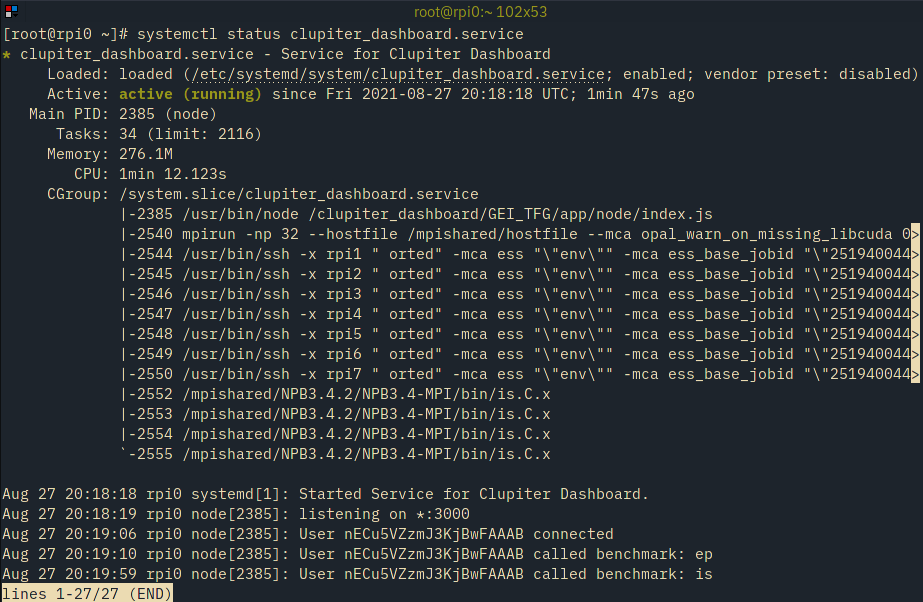
\includegraphics[width=0.9\textwidth]{img/systemd_clupiter_dashboard.png}
  \caption{Servicio \textit{Clupiter Dashboard} ejecutando un benchmark correctamente}
  \label{fig:systemd_clupiter_dashboard}
\end{figure}

% TODO IMAGEN DEL DASHBOARD

\chapter{Planificación y costes}
\label{chap:planificacion_costes}

\lettrine{E}{n} este penúltimo capítulo de la memoria se muestra una planificación detallada de la organización del proyecto, detalles acerca del método de trabajo, una lista de tareas, posteriormente ordenadas en un diagrama de Gantt, y un cálculo aproximado del coste del proyecto teniendo en cuenta el número de horas invertidas en las tareas desarrolladas, así como el coste de los elementos hardware adquiridos.

\section{Planificación del proyecto}
Durante el proceso de desarrollo de Clúpiter se ha seguido un modelo principalmente incremental. Las principales fases del proyecto se pueden dividir en las expuestas a continuación. Debe tenerse en cuenta que varias fases pueden solaparse debido a que la implementación hardware puede ir a un ritmo diferente a la software.

Salta a la vista la dilatación temporal de este \acrshort{tfg}, y es que la dedicación al mismo es superior en períodos vacacionales, e inferior durante el curso universitario, por evidentes razones. Además, en el agregado de los períodos vacacionales, se suman un total de cuatro semanas de descanso en las que no se ha trabajado en el proyecto. 

El sistema de comunicación con los directores del trabajo ha sido a través de Microsoft Teams. Las preguntas, dudas, aclaraciones, así como la corrección y comentarios de los diferentes capítulos de esta memoria han sido resueltos de forma principalmente asíncrona.

\subsection{Fase 1: Estudio de requisitos y compra de material}
En primer lugar se transmitió la necesidad por parte delos directores del trabajo de un proyecto orientado a docencia relacionado con la supercomputación, y un conjunto de ideas a realizar. Dichas ideas fueron combinadas en lo que ahora mismo es Clúpiter, altamente influenciadas por la coyuntura sanitaria causada por el COVID-19.

Tras esta aproximación inicial se elabora el presupuesto del clúster con vistas a la siguiente fase, y se procede a la compra del mismo. Como el tiempo de espera ante una compra por parte de la universidad es moderado, se comienza con la siguiente fase.

\subsection{Fase 2: Codiseño hardware/software}
Esta fase se puede dividir en dos disciplinas separadas, diseño hardware y diseño software. El diseño software es el primero en comenzar, realizándose la instalación del sistema Arch Linux en 4 máquinas virtuales que permitan ir testeando y scripteando todo lo requerido, eliminando las sorpresas a la hora de trabajar en infraestructura real.

Casi de forma simultánea, pero ligeramente más tarde, se comienza a diseñar en grano fino la estructura física de Clúpiter, realizando planos con medidas exactas, y renders del mismo.

\subsection{Fase 3: Implementación hardware/software}
Una vez la infraestructura se encuentra prácticamente desplegada al completo en máquinas virtuales, se comienza con el montaje de Clúpiter. Primero se comprueba la calidad de todos los componentes hardware. Tras ello se cortan las planchas de chapa que unen las diferentes secciones verticales del clúster, y finalmente se realiza el ensamblaje final y corte del cableado a medida, tal y como se comenta en \nameref{sec:configuracion_hardware}.

Una vez montado por completo el clúster, se instala ArchLinuxARM en cada uno de los nodos, como se explica previamente en \nameref{sec:configuracion_software}, y se realizan todos los pasos descritos en dicha sección. Este proceso, tal como se comentaba previamente, transcurre sin sorpresas debido a la experiencia previa con las máquinas virtuales, siendo la única diferencia el método de instalación del propio sistema.

\subsection{Fase 4: Medida del rendimiento}
En un principio se ejecutan los \acrlong{npb} sobre la infraestructura virtual, por lo que gran parte del camino ya está allanado para la implementación en el hardware final. Por esta razón esta fase también transcurre sin gran cantidad de problemas. Estos pocos problemas que se encontraron, estaban relacionados con limitaciones de espacio en memoria, que se solucionaron bajando la clase del problema, como se discute en el Capítulo \ref{chap:medida_rendimiento}.

Para la recolección de datos se programa un script con el que llevar a cabo múltiples ejecuciones de los benchmarks de forma automatizada (las cuales consumen un tiempo importante), y almacenar la salida por pantalla de los mismos. Al terminar se ordenan, procesan e interpretan.

\subsection{Fase 5: Desarrollo del dashboard}
El desarrollo del dashboard ha sido uno de los puntos más difíciles desde el punto de vista del diseño, ya que no es tan sencillo como pueda parecer el pensar cómo se va a explicar a una persona sin grandes conocimientos de informática, cómo funciona un clúster, y por qué es importante.

Inicialmente se diseña un primer prototipo de la aplicación de monitorización en Python con la librería gráfica GTK y Matplotlib (pyplot), pero, tras recibir el \textit{feedback} de personas cercanas al desarrollo web, finalmente se opta por no continuar con su desarrollo en favor de una variante basada en tecnologías web.

Al final, tras bastante prototipado y consultas con personas que podrían ser el objetivo de dichas explicaciones, se ha optado por el diseño del dashboard discutido en el Capítulo \ref{chap:aplicacion_web}.

\subsection{Fase 6: Documentación, redacción y retoques}
La documentación y escritura de la memoria se inicia casi desde el principio del proyecto, ya que, a medida que se va avanzando en el mismo, se van tomando anotaciones que faciliten su posterior escritura, así como para servir de recordatorio de los pasos dados. Una vez finalizado el proyecto, se procede a darle estructura a todas esas anotaciones, esto es:
\begin{itemize}
    \item Añadir \textbf{``literatura''}, es decir, cohesionar todo el texto, y explicar de forma más correcta las anotaciones realizadas durante el proceso de desarrollo.
    \item Añadir \textbf{citas} a páginas web y artículos que se leyeron en su momento y fueron consecuentemente guardados en el archivo de bibliografía, así como \textbf{buscar artículos} que sustenten afirmaciones basadas en la experiencia.
    \item \textbf{Crear figuras} explicativas, así como ordenar las múltiples fotografías tomadas a lo largo del proyecto.
    \item \textbf{Guionizar} y \textbf{preparar} los \textbf{vídeos} a incluír en el dashboard.
\end{itemize}

Al finalizar la redacción de la memoria se realizan los últimos retoques y revisiones en la misma, se termina de refinar el dashboard (por ejemplo, traduciendo todo al castellano), y se graban los vídeos que van insertados en el mismo.

\section{Métricas del proyecto}
En esta sección se desglosan las tareas en cada fase, se desarrolla un diagrama de Gantt y se realiza un cálculo teórico del coste total del proyecto.

\subsection{Desglose de tareas}
En esta sección se detallan las principales tareas que han sido llevadas a cabo en cada una de estas fases y su coste final en horas. El proyecto está programado para ser ejecutado en alrededor de 300 horas (12 créditos ECTS), distribuídas entre las fases previamente comentadas.

En la Tabla \ref{tab:desglose_de_tareas} se puede ver el desglose de tareas y su coste en h$\times$h. Además, para poder referenciar las tareas en el texto, se asigna un \acrshort{tid} (\textit{\acrlong{tid}}) alfanumérico a cada una de ellas. 
\begin{table}[htpb]
  \centering
  \begin{tabular}{ |c|c|c|c| }
  \hline
  \textbf{Fase} & \textbf{TID} & \textbf{Tarea} & \textbf{Tiempo (h)} \\ 
  \hline
  % Fase 1
  \multirow{4}{*}{1}        & a     & {Reunión inicial y exposición de la propuesta}                            & 2 \\\cline{2-4}
                            & b     & {Estudio de proyectos similares y estimación inicial}                     & 8 \\\cline{2-4}
                            & c     & {Análisis de requisitos}                                                  & 8 \\\cline{2-4}
                            & d     & {Presupuestado}                                                           & 2 \\
  \hline
  % Fase 2
  \multirow{3}{*}{2}        & e     & {Preparación de la infraestructura virtual}                               & 2 \\\cline{2-4}
                            & f     & {Investigación en máquinas virtuales}                                     & 20 \\\cline{2-4}
                            & h     & {Diseño estructural del hardware}                                         & 6 \\
  \hline
  % Fase 3
  \multirow{5}{*}{3}        & i     & {Testeo y puesta a punto del hardware}                                     & 8 \\\cline{2-4}
                            & j     & {Cortado, lijado y pintado del chasis}                                    & 3 \\\cline{2-4}
                            & k     & {Montaje y solución de problemas}                                         & 16 \\\cline{2-4}
                            & l     & {Despliegue del sistema}                                                  & 16 \\\cline{2-4}
                            & m     & {Adaptación del sistema y solución de problemas}                          & 6 \\
  \hline
  % Fase 4
  \multirow{3}{*}{4}        & n     & {Investigación y prueba de los NPB}                                       & 8 \\\cline{2-4}
                            & o     & {Despliegue de los NPB}                                                  & 4 \\\cline{2-4}
                            & p     & {Medida del rendimiento y obtención de resultados}                        & 24 \\
  \hline
  % Fase 5
  \multirow{3}{*}{5}        & g     & {Diseño general y primeros prototipos en papel}                           & 18 \\\cline{2-4}
                            & q     & {Investigación tecnologías web}                                           & 4 \\\cline{2-4}
                            & r     & {Diseño e implementación dashboard}                                       & 30 \\
  \hline
  % Fase 6
  \multirow{4}{*}{6}        & s     & {Redacción de la memoria}                                                 & 100 \\\cline{2-4}
                            & t     & {Maquetado y relacionados}                                                & 12 \\\cline{2-4}
                            & u     & {Grabación de los vídeos}                                                 & 12 \\\cline{2-4}
                            & v     & {Traducción y puesta a punto del dashboard}                               & 4 \\
  \hhline{|=|=|=|=|}
  \multicolumn{3}{|c|}{\textbf{Total}}                                                                          & \textbf{313}\\
  \hline
  \end{tabular}
  \caption{Desglose de tareas por fase y coste en h$\times$h}
  \label{tab:desglose_de_tareas}
\end{table}

\subsection{Diagrama de Gantt}
La duración de este proyecto ha sido de poco más de un año natural, debido a que la dedicación en horas/semana ha sido bastante variable. Durante el curso académico hay escaso tiempo y motivación para dedicarle al \acrshort{tfg}, siendo esta última escasa en una situación de pandemia y teledocencia. Por otro lado, durante los períodos vacacionales es donde se encuentran concentradas la mayor cantidad de horas de trabajo. Por ello, la longitud de las tareas en el diagrama de Gantt no es proporcional al número de h$\times$h (horas por hombre) adjudicadas a las mismas si se asumiese una jornada de trabajo estable.

La Figura \ref{fig:diagrama_gantt} muestra el diagrama de Gantt, que ilustra cómo se desarrolló el proyecto en el tiempo y las relaciones de predecencia entre tareas.

\subsection{Presupuesto}
Durante el desarrollo del proyecto han realizado diferentes trabajos tres personas: el estudiante, encargado de la gestión del ciclo de vida del proyecto y de llevar todas sus fases a cabo, y los dos tutores, encargados de la proposición del proto-proyecto y de la supervisión durante el desarrollo del mismo.

En la Tabla \ref{tab:horas_recurso} se puede encontrar una relación aproximada de las horas invertidas en el proyecto por cada recurso involucrado en el desarrollo y supervisión del mismo.

\begin{table}[h!]
  \centering
  \begin{tabular}{ |c|c| }
  \hline
  \textbf{Recurso} & \textbf{Dedicación (h)} \\ 
  \hline
  Estudiante       & 313\\
  \hline
  Tutor 1          & 30\\
  \hline
  Tutor 2          & 20\\
  \hline
  \end{tabular}
  \caption{Horas invertidas en el proyecto por recurso}
  \label{tab:horas_recurso}
\end{table}

Por último, en la Tabla \ref{tab:coste_total} puede encontrarse la suma de tanto los costes humanos, como los del equipamiento hardware adquirido.

\begin{table}[h!]
  \centering
  \begin{tabular}{ |c|c|c|c| }
  \hline
  \textbf{Recurso} & \textbf{Coste por hora (\small\officialeuro\normalsize)} & \textbf{Horas} & \textbf{Coste (\small\officialeuro\normalsize)} \\ 
  \hline
  Estudiante       & 30     & 313       & 9390\\
  \hline
  Tutor 1          & 60     & 30        & 1800\\
  \hline
  Tutor 2          & 60     & 20        & 1200\\
  \hhline{|=|=|=|=|}
  \multicolumn{3}{|c|}{\textbf{Material}} & \textbf{--}\\
  \hline
  \multicolumn{3}{|c|}{Prespuesto inicial} & 841.68\\
  \hline
  \multicolumn{3}{|c|}{Cables USB-C magnéticos} & 26.16\\
  \hline
  \multicolumn{3}{|c|}{Step-up MT3608} & 1.79\\
  \hhline{|===|=|}
  \multicolumn{3}{|c|}{\textbf{Total}} & \textbf{13259.63 (\small\officialeuro\normalsize)}\\
  \hline
  \end{tabular}
  \caption{Coste total de Clúpiter}
  \label{tab:coste_total}
\end{table}

\begin{landscape}
\begin{figure}
    \centering
    \resizebox{\linewidth}{!}{
        \centering
        \begin{ganttchart}[
            time slot format=isodate,
            hgrid, vgrid={*{7}{draw=none},dotted},
            x unit=0.09cm,
            y unit title=1cm,
            y unit chart=0.7cm,
            title/.append style={shape=rectangle, fill=black!10},
            title height=1,
            link/.append style={-stealth,draw=black},
            group/.append style={fill=ficblue},
            bar/.append style={fill=udcpink!35,draw=udcpink},
            milestone/.append style={fill=ficblue!35,draw=ficblue,xscale=4}
        ] {2020-8-12}{2021-09-21}
            \gantttitlecalendar{year}\\
            \gantttitlecalendar{month=name}\\
            % Aquí cambio junio por agosto, ya que es poco relevante dejar un mes y medio en blanco porque estuve de vacaciones fuera
            \ganttgroup{Fase 1}{2020-8-15}{2020-8-25}\\
            % reunion
            \ganttbar[name=a]{Tarea a}{2020-8-15}{2020-8-15}\\
            % estudio de proyectos similares
            \ganttbar[name=b]{Tarea b}{2020-8-16}{2020-8-21}\\
            % analisis de requisitos
            \ganttbar[name=c]{Tarea c}{2020-8-22}{2020-8-24}\\
            % presupuestado
            \ganttbar[name=d]{Tarea d}{2020-8-25}{2020-8-25}\\

            \ganttgroup{Fase 2}{2020-8-30}{2020-10-1}\\
            % preparación vm
            \ganttbar[name=e]{Tarea e}{2020-8-30}{2020-9-1}\\
            % investigación en vm
            \ganttbar[name=f]{Tarea f}{2020-9-2}{2020-9-15}\\
            % diseño estructural del hardware
            \ganttbar[name=h]{Tarea h}{2020-9-25}{2020-10-1}\\


            % HITO recepción material
            \ganttmilestone[name=rec_material]{Recepción del material}{2020-10-6}\\


            \ganttgroup{Fase 3}{2020-11-5}{2021-6-26}\\
            % testeo y puesta a punto del hardware
            \ganttbar[name=i]{Tarea i}{2020-11-5}{2020-11-7}\\
            % cortado, lijado y pintado del chasis
            \ganttbar[name=j]{Tarea j}{2020-11-8}{2020-11-8}\\
            % montaje y solución de problemas
            \ganttbar[name=k]{Tarea k}{2021-1-3}{2021-1-10}\\
            % despliegue del sistema
            \ganttbar[name=l]{Tarea l}{2021-6-21}{2021-6-23}\\
            % adaptación del sistema
            \ganttbar[name=m]{Tarea m}{2021-6-24}{2021-6-26}\\


            \ganttgroup{Fase 4}{2021-4-25}{2021-7-15}\\
            % investigación acerca de los npb
            \ganttbar[name=n]{Tarea n}{2021-4-25}{2021-5-10}\\
            % despliegue de los npb
            \ganttbar[name=o]{Tarea o}{2021-6-29}{2021-7-2}\\
            % medida del rendimiento y obtención de resultados
            \ganttbar[name=p]{Tarea p}{2021-7-4}{2021-7-15}\\

            \ganttgroup{Fase 5}{2020-9-10}{2021-7-18}\\
            % diseño general y primeros prototipos
            \ganttbar[name=g]{Tarea g}{2020-9-10}{2020-10-15}\\
            % investigación tecnologías web
            \ganttbar[name=q]{Tarea q}{2021-7-3}{2021-7-4}\\
            % diseño e implementación dashboard
            \ganttbar[name=r]{Tarea r}{2021-7-5}{2021-7-18}\\

            \ganttgroup{Fase 6}{2021-6-18}{2021-9-11}\\
            % redacción de la memoria
            \ganttbar[name=s]{Tarea s}{2021-6-18}{2021-9-5}\\
            % maquetado y relacionados
            \ganttbar[name=t]{Tarea t}{2021-9-6}{2021-9-11}\\
            % grabación de los vídeos
            \ganttbar[name=u]{Tarea u}{2021-9-8}{2021-9-10}\\
            % traducción y puesta a punto del dashboard
            \ganttbar[name=v]{Tarea v}{2021-9-9}{2021-9-11}\\


            
            % GANTTLINKS

            \ganttlink[link type=F-S]{a}{b}
            \ganttlink[link type=F-S]{b}{c}
            \ganttlink[link type=F-S]{c}{d}

            \ganttlink[link type=F-S]{c}{e}
            \ganttlink[link type=F-S]{e}{f}
            \ganttlink[link type=F-S]{e}{n}
            \ganttlink[link type=F-S]{f}{l}

            \ganttlink[link type=F_S]{c}{g}
            \ganttlink[link type=F-S]{h}{rec_material}

            \ganttlink[link type=F-S]{d}{h}

            \ganttlink[link type=F-S]{d}{rec_material}

            \ganttlink[link type=F-S]{rec_material}{i}
            \ganttlink[link type=F-S]{rec_material}{j}

            \ganttlink[link type=F-S]{i}{k}
            \ganttlink[link type=F-S]{j}{k}

            \ganttlink[link type=F-S]{k}{l}
            \ganttlink[link type=F-S]{l}{m}

            \ganttlink[link type=F_S]{m}{o}
            \ganttlink[link type=F_S]{m}{r}


            \ganttlink[link type=F-S]{n}{o}
            \ganttlink[link type=F-S]{o}{p}


            \ganttlink[link type=F-S]{g}{q}
            \ganttlink[link type=F-S]{q}{r}


            \ganttlink[link type=F-S]{s}{t}

            \ganttlink[link type=F_S]{s}{v}
            \ganttlink[link type=F_S]{s}{u}


            \ganttlink[link type=F-F]{p}{s}
            \ganttlink[link type=F-F]{r}{s}
            \ganttlink[link type=F-F]{v}{t}
            \ganttlink[link type=F-F]{u}{v}
        \end{ganttchart}
    }
    \caption{Diagrama de Gantt del desarrollo de Clúpiter}
    \label{fig:diagrama_gantt}
\end{figure}
\end{landscape}
\chapter{Conclusiones}
\label{chap:conclusiones}

\lettrine{E}{n} este último capítulo se hace un balance general de este \acrlong{tfg}, a partir del cual se extraen conclusiones, así como su relación con la titulación y posibles líneas de trabajo futuro, algunas de las cuales ya se han mencionado previamente a lo largo de todo el documento.

\section{Conclusiones}
El objetivo del \acrshort{tfg} es la creación de un mini-supercomputador con \acrlong{rpi}s, que sirva como base tangible para realizar explicaciones a personas con poca o ninguna formación en este sector del \acrshort{hpc}. Personalmente, y dejando siempre espacio para la discrepancia de los profesores que lo evalúen, pienso que este objetivo se ha cumplido con creces, puesto que el resultado ha sido un supercomputador en miniatura, con todas sus secciones bien diferenciadas, y extrapolables a un supercomputador real. 

Por otro lado, en el apartado software se ha puesto mucho énfasis en la simplicidad tanto de implementación como de mantenimiento, intentando realizar las configuraciones necesarias siempre con la mínima cantidad de dependencias y condicionantes posibles. Además, el dashboard, si bien no es una pieza de código particularmente compleja, tiene invertidas una gran cantidad de horas en diseño, especialmente de cara a la docencia y divulgación. A primera vista éstas pueden no parecer evidentes, pero se notan cuando uno se fija más en detalle y emplea adecuadamente los recursos que el dashboard ofrece.

En cuanto a rendimiento y escalabilidad, se puede concluir con total seguridad que quizás, para \acrshort{hpc}, la plataforma de la frambuesa no es la más adecuada. Esto no debería coger a nadie por sorpresa, ya que no existen componentes redundantes en todo el clúster (ni posibilidad de añadirlos), hay una falta importante de aceleración por hardware y, en general, ninguna \acrlong{rpi} está diseñada para ser un ordenador especialmente eficaz en este sentido (véase especialmente el impacto del ancho de banda a la memoria principal en la sección \ref{sec:comparacion_resultados}). Sin embargo, esto no quita que los test de rendimiento se puedan ejecutar sobre esta plataforma y medir el impacto de los diversos componentes de la misma sobre el resultado final, que es, como mínimo, decepcionante.

Personalmente, este \acrshort{tfg} me ha permitido llevar a cabo algo que siempre despertó mi curiosidad, pero que por cuestiones económicas nunca fue una opción realizar. En este sentido, ya tenía información previa en forma de vídeos de YouTube. Por otro lado, al ser un proyecto que abarca varias áreas de la informática, me ha permitido poner en práctica diversas capacidades aprendidas durante la carrera, las cuales me han permitido no solo saber qué hacer en qué momento, sino tener la capacidad de poder visualizar posibles líneas de evolución para posibles nuevas iteraciones de este proyecto, y diseñar con vistas a ello.

\section{Relación con la titulación}
Durante el desarrollo de Clúpiter se pusieron en práctica ciertas habilidades y conocimientos aprendidos tanto en la carrera como a raíz de la misma. En concreto estas habilidades van en relación con las asignaturas relacionadas con administración de infraestructuras (\acrshort{aii} y \acrshort{eii}), administración y gestión de sistemas operativos (\acrshort{ib}, \acrshort{so}, \acrshort{aso}, \acrshort{aii}), gestión de redes (\acrshort{ib}, redes, \acrshort{ar}), gestión de proyectos, especialmente procesos software (\acrshort{xp} y \acrshort{ps}), así como programación paralela con \acrshort{mpi} (\acrshort{cp} y \acrshort{ac}). Además, me gustaría hacer mención especial a asignaturas como \acrshort{fc}, \acrshort{ec}, \acrshort{ac}, \acrshort{te}, \acrshort{dhi}, \acrshort{cp}, \acrshort{se} y \acrshort{chs} por ser una inspiración a lo largo de la carrera, y que en parte han hecho que me decante por este proyecto\footnote{Puede encontrarse la relación de estas asignaturas con su nombre completo en la lista de acrónimos}.

Por otro lado, también es positiva la dinámica que imbuye la carrera en los estudiantes de la misma, que, si bien en mi caso ya era autodidacta desde bien pequeño, anima y obliga a ``salir de la zona de confort'' a los estudiantes, resultando eso de gran ayuda al afrontar proyectos en los que se desconoce qué tecnologías usar, así como a la hora de aprender a usar las mismas.

\section{Trabajo futuro}
Como se viene comentando a lo largo de todo el documento, hay múltiples líneas de trabajo con las que continuar. Estas posibles ``iteraciones'' adicionales deberían seguir en sí mismas un ciclo de vida incremental, dando así un ciclo de vida iterativo al propio Clúpiter, siendo esta la versión 1.0, por ejemplo.

En un ánimo de proponer mejoras o modificaciones que realizar en hipotéticas iteraciones futuras, se pueden encontrar:
\begin{itemize}
    \item Mejora del rendimiento de la CPU mediante \gls{overclock}.
    \item Mejora del ancho de banda de la memoria principal, tambien mediante \gls{overclock}.
    \item Mejora de la seguridad del sistema.
    \item Mejora y automatización de la mantenibilidad del sistema.
    \item Mejora del chasis, especialmente mediante el uso de una plegadora en el cortado de las planchas.
    \item Mejora del dashboard, preferiblemente extendiendo su funcionalidad y no modificándola.
    \item Implementar sincronización precisa de la hora. Esto podría ser necesario ya que ahora mismo se restaura la hora del último apagado, permitiendo hasta un máximo de 2 minutos de desfase entre relojes por apagado. Esto es inofensivo debido a que no se emplea SSL/TLS, ni hay bloqueo de archivos en NFS, ya que es solo lectura para los clientes. Sin embargo, en un futuro podría cambiarse esto, y debe ser un punto a tener en cuenta.
\end{itemize}

Finalmente, una iteración que personalmente me haría ilusión que alguien realizase, consistiría en acelerar el rendimiento de algún programa computacionalmente exigente mediante la GPU/VPU VideoCore VI (\ref{ssec:gpu_vpu}). Esto, que requiere una investigación más en profundidad por parte de un hipotético interesado, quizás podría realizarse mediante Vulkan Compute Shaders, OpenCL si este estuviese disponible en ese momento, o empleando alguna librería como py-videocore6\footnote{\url{https://github.com/Idein/py-videocore6}}, pareciéndome la primera la opción más interesante.

%%%%%%%%%%%%%%%%%%%%%%%%%%%%%%%%%%%%%%%%
% Apéndices, glosarios e bibliografía  %
%%%%%%%%%%%%%%%%%%%%%%%%%%%%%%%%%%%%%%%%

\appendix
\appendixpage
\chapter{Factsheet on the Digital Europe Programme}
\label{chap:factsheet_europe}

\lettrine{E}{n} las siguientes dos páginas se adjunta una copia del documento publicado por la Unión Europea tratando la inversión a realizar en inteligencia artificial, ciberseguridad, pero, sobre todo, en supercomputación.

% Left Bottom Right Top
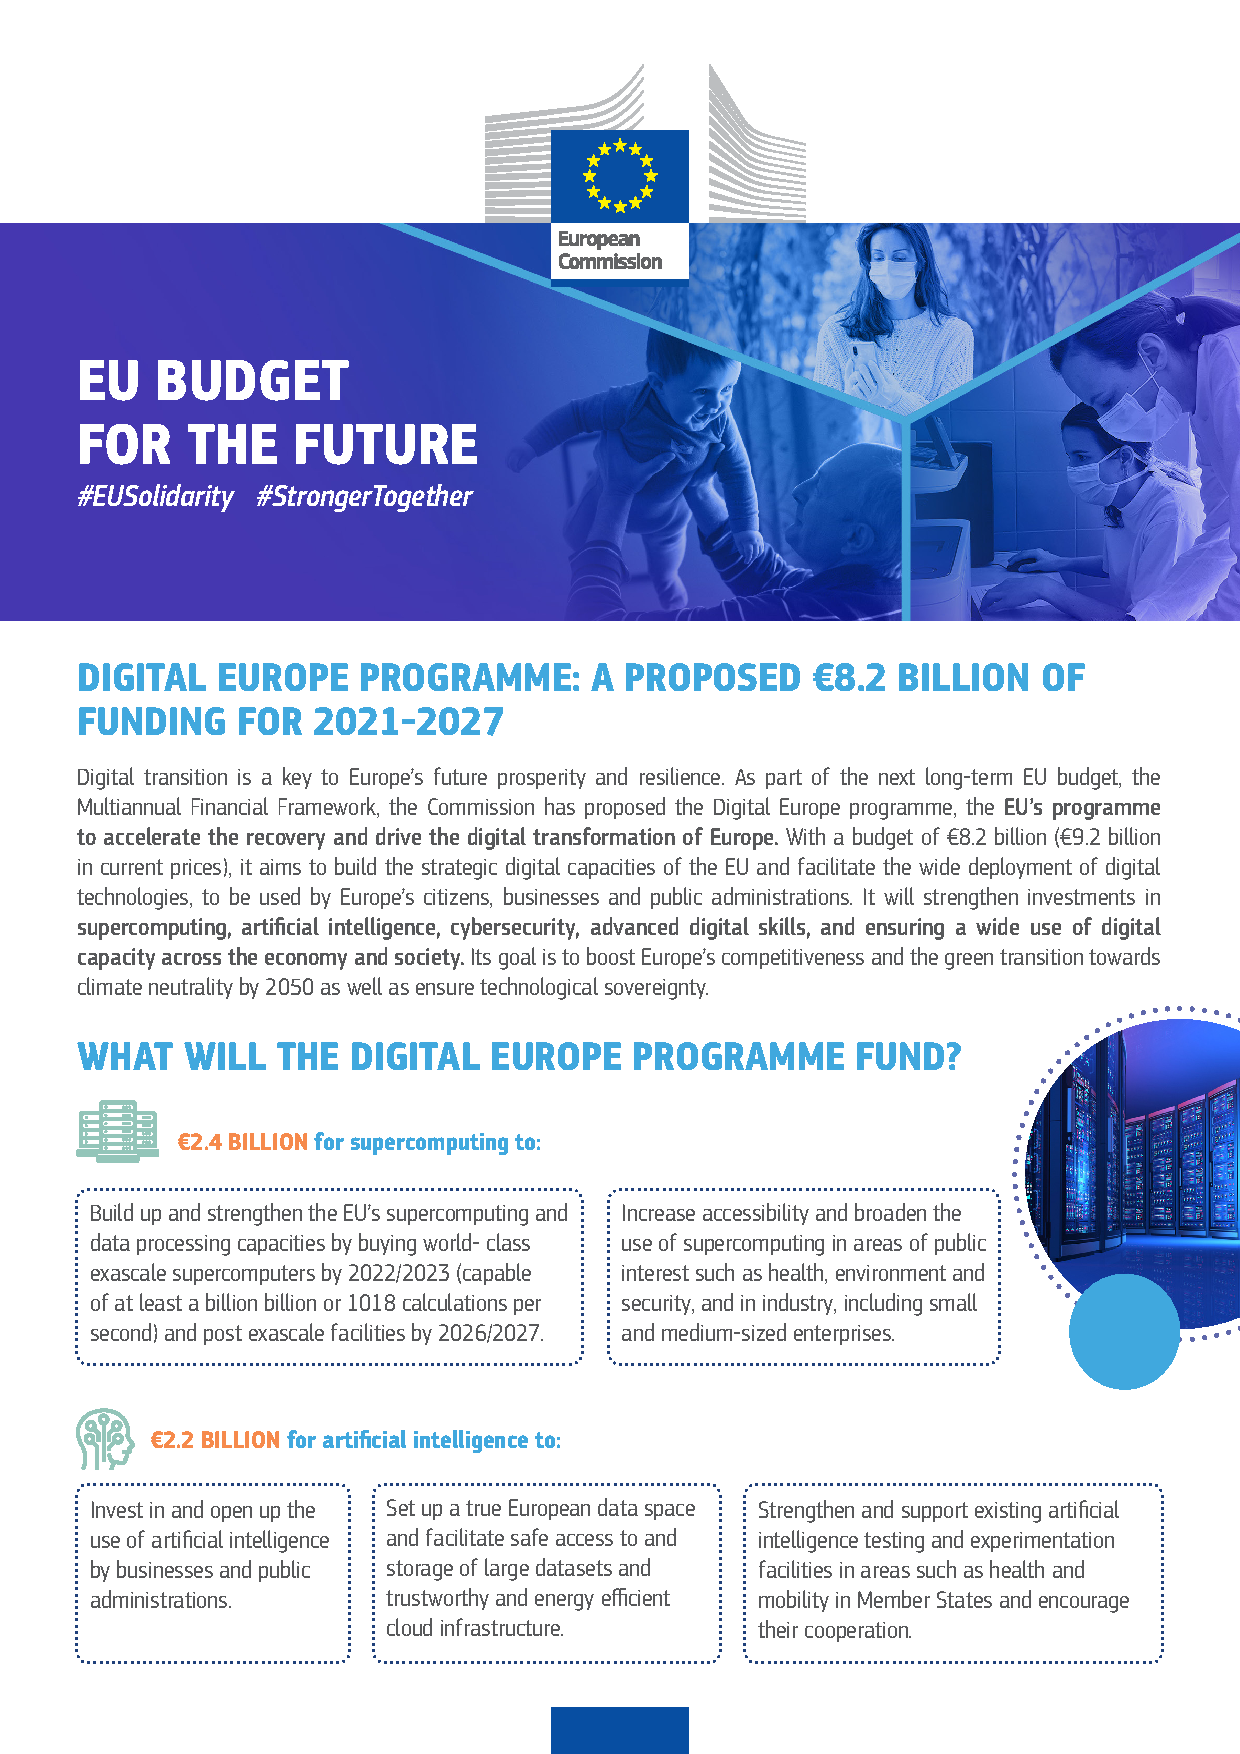
\includepdf[pages={1-}]{pdf_tex/factsheet_europe/FactsheetontheDigitalEuropeProgramme.pdf}
\chapter{Resultados de los NPB}
\label{chap:bench_values}

\lettrine{E}{n} este anexo se adjunta una copia de los valores de cada ejecución de los \acrlong{npb}.

En concreto, dichos datos se encuentran en la siguiente página, y el tamaño de los mismos está pensado para ser visualizado en ordenador, donde puede ampliarse el zoom del visualizador. Si está leyendo una versión escrita, por favor diríjase a la versión digital de esta misma publicación.

% Left Bottom Right Top
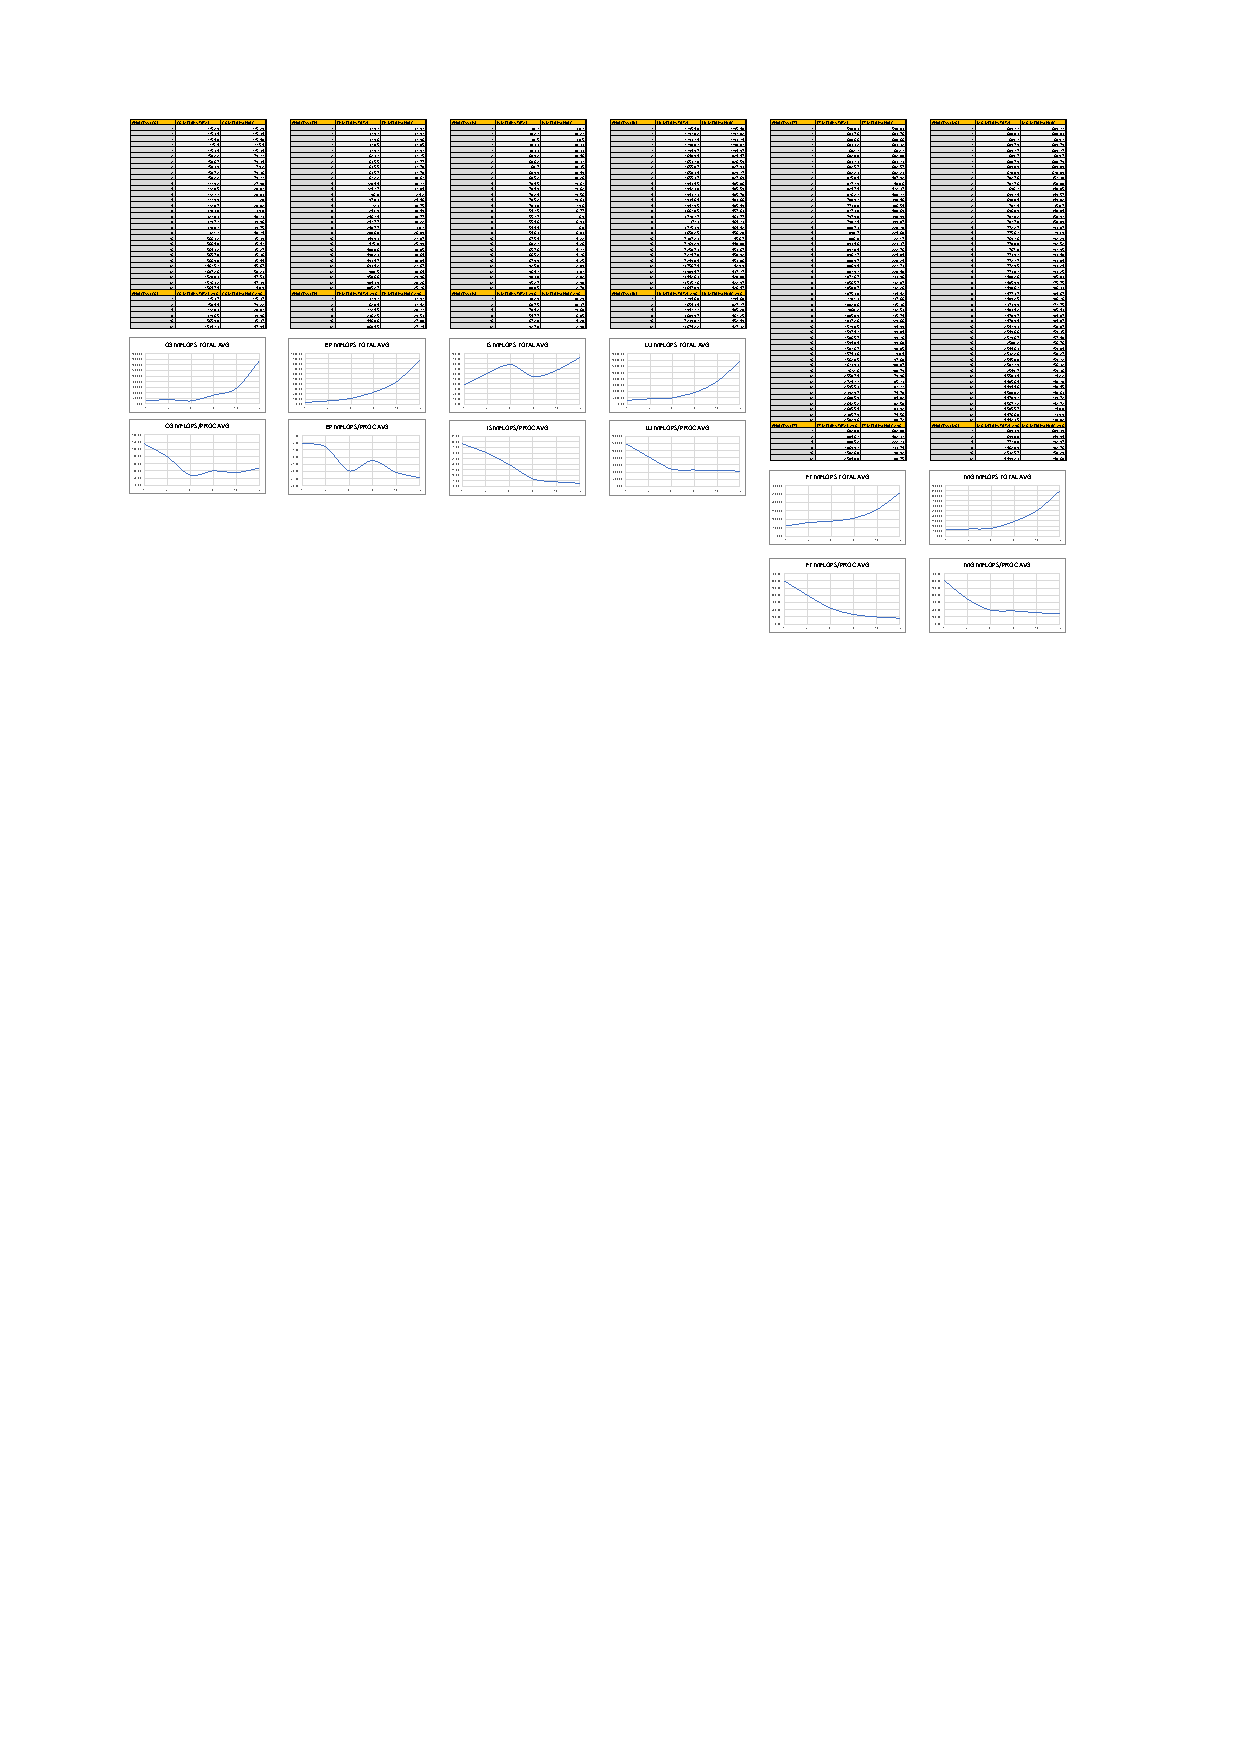
\includepdf[landscape,trim=02mm 190mm 10mm 20mm]{pdf_tex/bench_values/values.pdf}
%\chapter{Presupuesto de Clúpiter}
\label{chap:presupuesto_clupiter}

\lettrine{E}{n} la siguiente página se adjunta una copia del presupuesto de Clúpiter. A éste hay que añadir los cables magnéticos comprados posterioremente:

\begin{figure}[H]
  \centering
  \vspace{0.5cm}
  % Left Bottom Right Top
  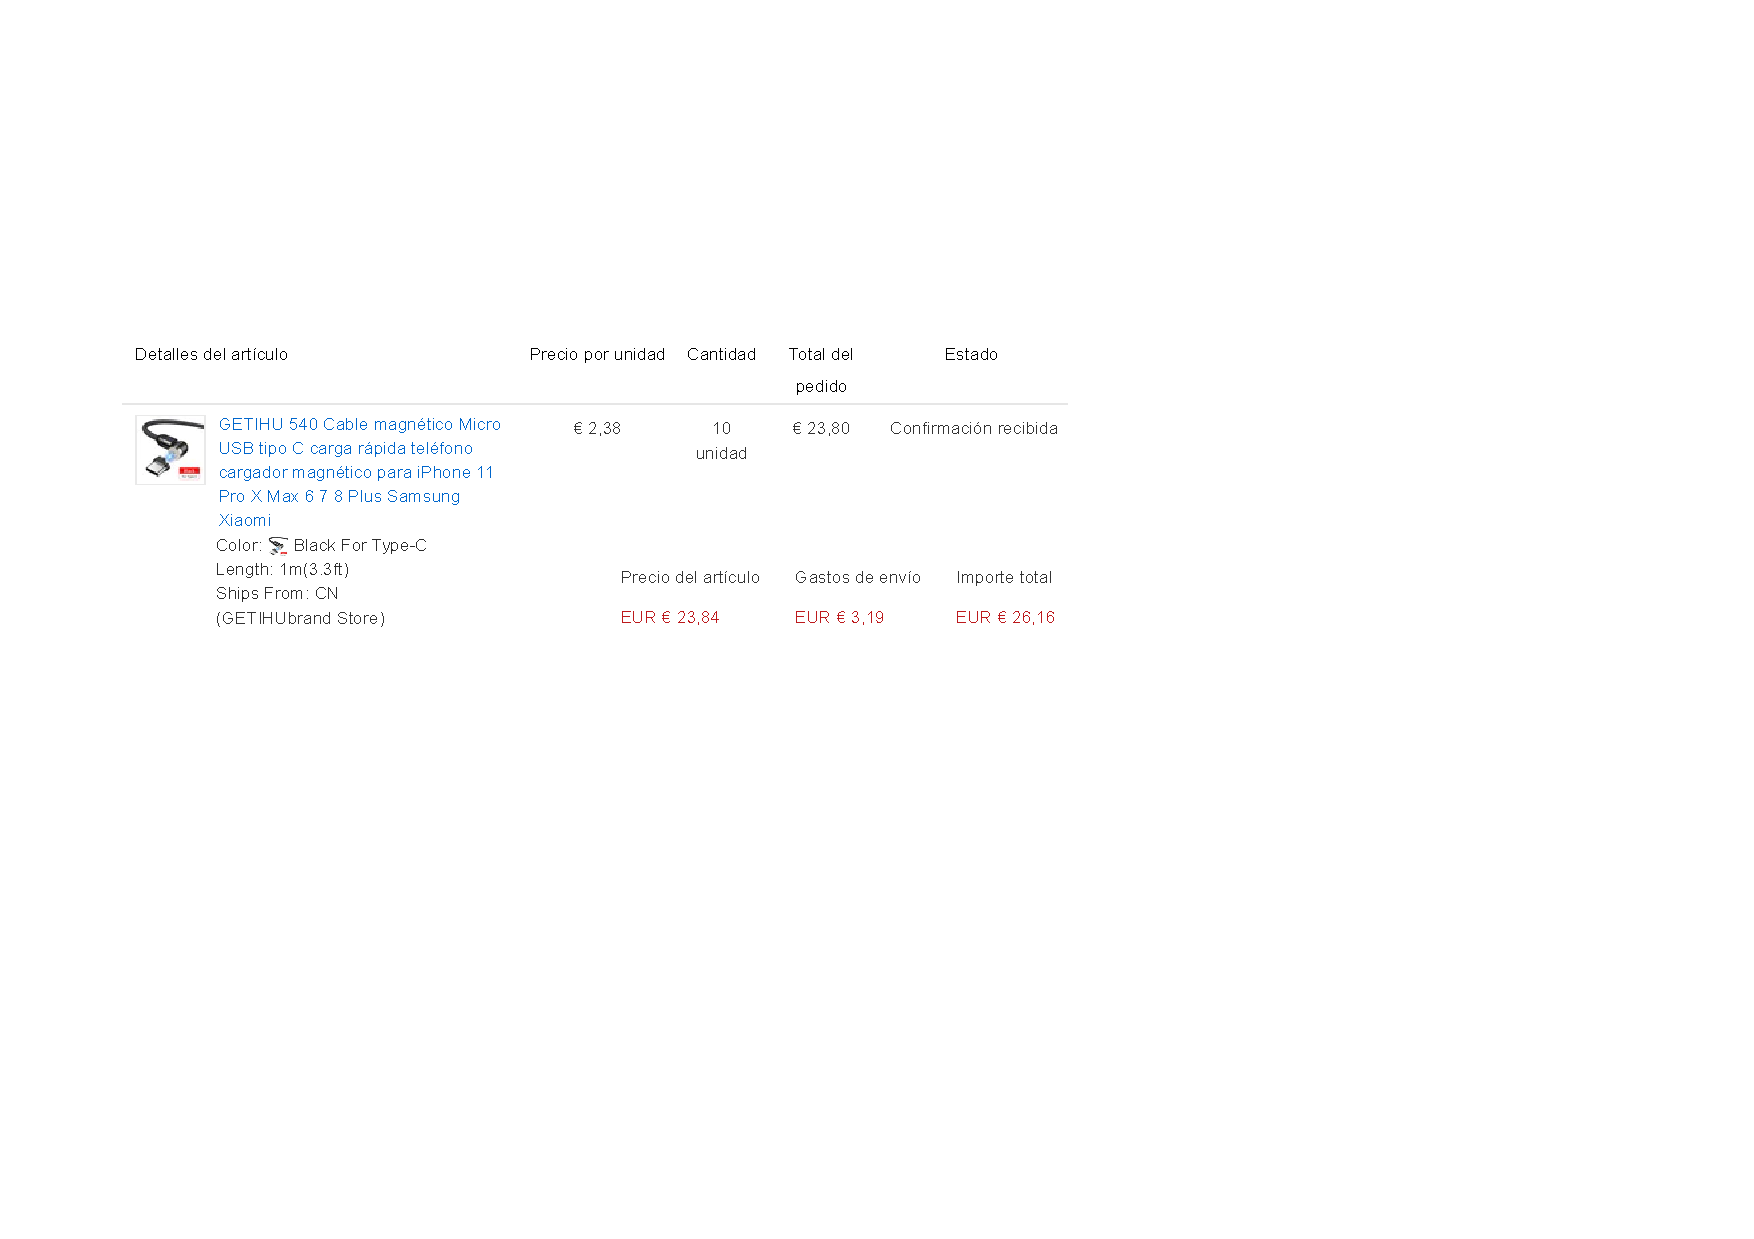
\includegraphics[width=\textwidth,trim=18mm 98mm 113mm 57mm]{pdf_tex/presupuesto_clupiter/getihu_cable.pdf}
\end{figure}

% Left Bottom Right Top
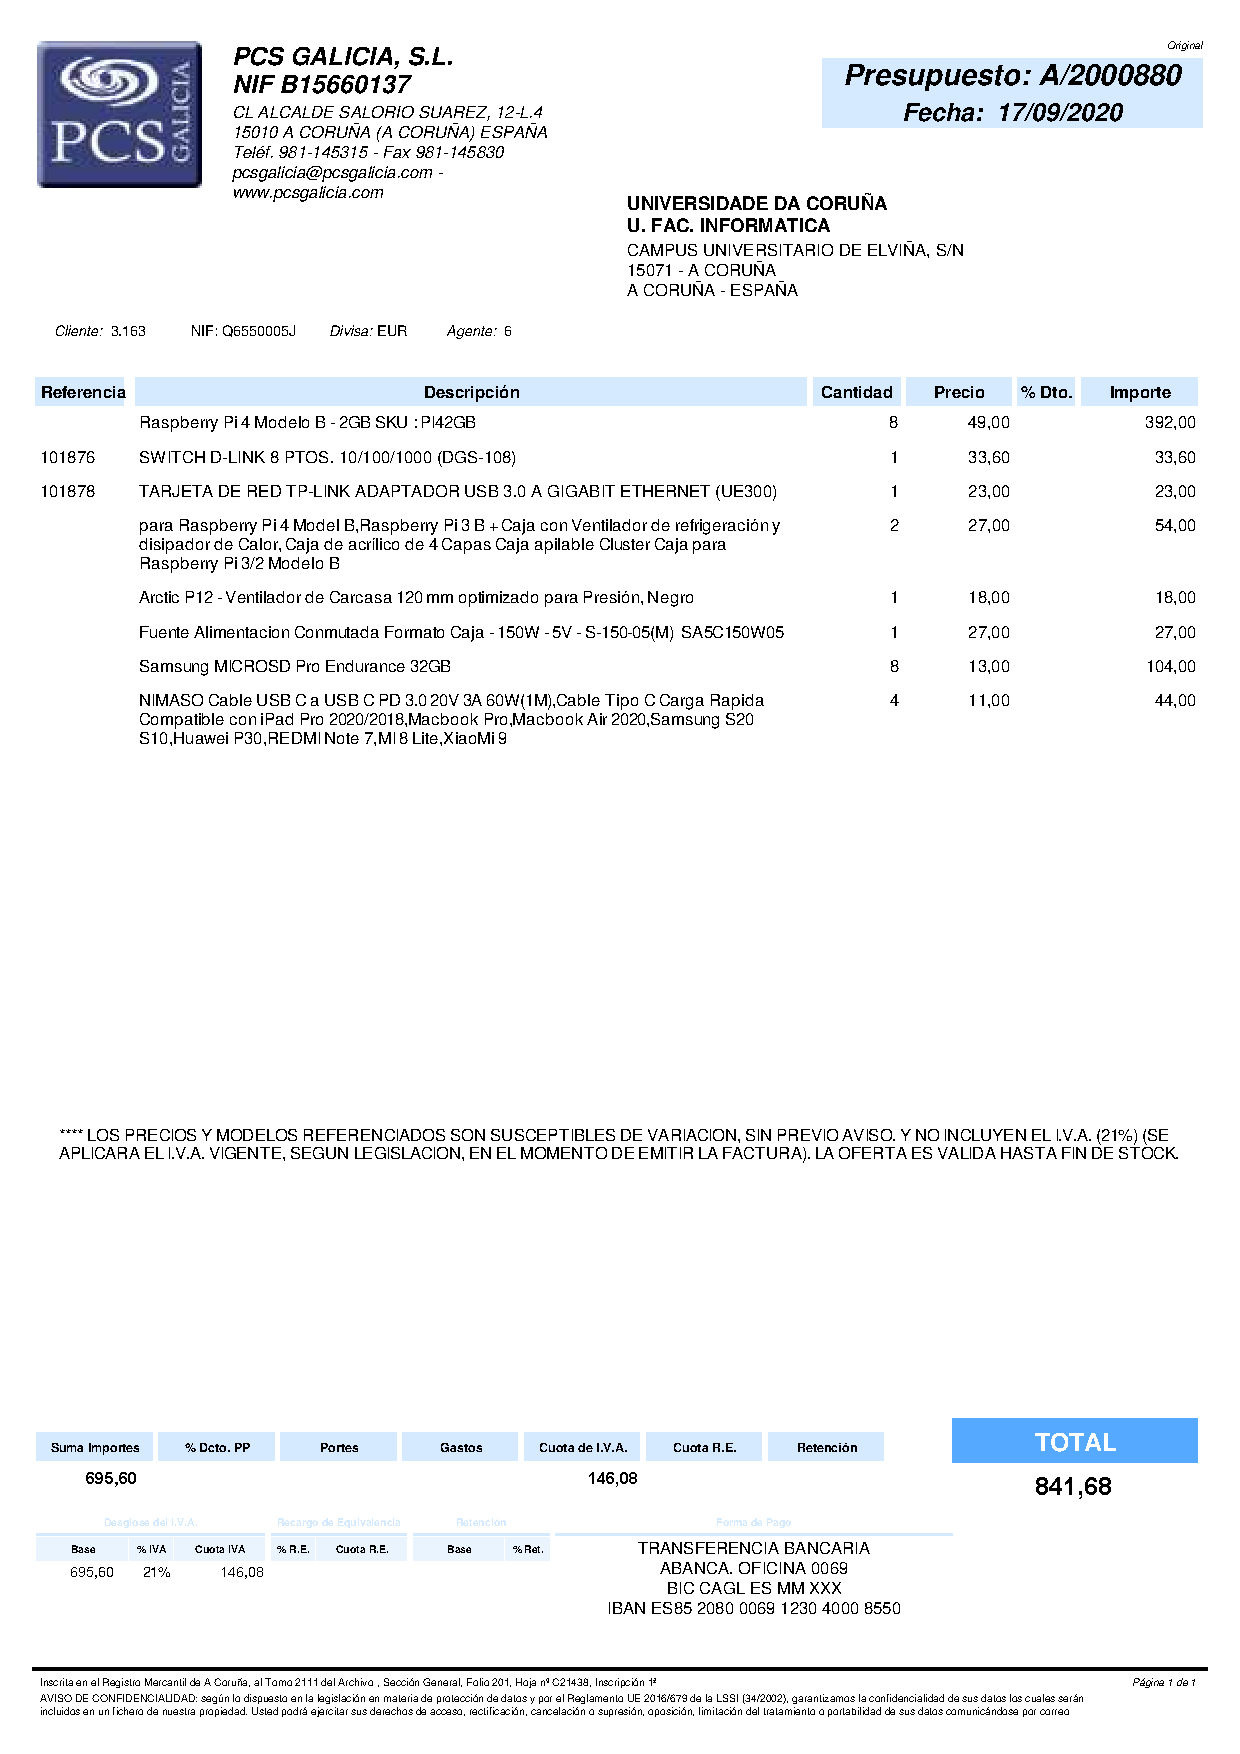
\includepdf[]{pdf_tex/presupuesto_clupiter/Presupuesto_PCS_Galicia_(C).pdf}
\chapter{Guía de mantenimiento de Arch Linux}
\label{chap:archlinux_maintenance_guide}

\lettrine{E}{n} este apéndice se encuentra una breve guía de los comandos más básicos para mantener Clúpiter a punto, especialmente haciendo enfoque en las actualizaciones y mantenimiento básico del sistema.

\section{Enlaces de interés}
Ante cualquier duda, consulta, o problema, se debe acudir a la wiki de Arch Linux, donde lo más probable es que se encuentre la respuesta. A continuación se muestra una lista de entradas relevantes de esta wiki y similares:

\begin{itemize}
    \item Introducción a Arch Linux, donde en especial se recomienda la sección ``Package management''.
    \url{https://wiki.archlinux.org/title/General_recommendations}

    \item Arch User Repository. Este es un repositorio gestionado por la comunidad, donde se pueden encontrar gran cantidad de paquetes no soportados oficialmente, pero que habitualmente cuentan con un soporte de calidad. En caso de emplearse de forma asidura, se recomienda instalar un \textit{wrapper} de AUR, como por ejemplo \texttt{yay} o \texttt{paru}.\\
    \url{https://wiki.archlinux.org/title/Arch_User_Repository}

    \item Manual para systemd: \url{https://wiki.archlinux.org/title/Systemd}.
    \item Configuración de red: \url{https://wiki.archlinux.org/title/Systemd-networkd}.
    \item Configuraciones para \acrlong{rpi}: \\\url{https://archlinuxarm.org/wiki/Raspberry_Pi}.

    \item Manual de pacman, el gestor de paquetes de Arch Linux: \\\url{https://wiki.archlinux.org/title/General_recommendations}
\end{itemize}

Para un usuario más novato esto podría parecer abrumados en un principio, pero desde mi punto de vista esta la mejor forma de aprender, y el espíritu que promueve Arch Linux. 

\section{Actualización del sistema}
Si se han leido con detenimiento las entradas en la sección anterior no debería haber mucha duda en qué hacer para actualizar el sistema. Sin embargo, siembre vienen bien las recomendaciones basadas en la experiencia.

Como Clúpiter probablemente se actualice muy de vez en cuando, es necesario tomar precauciones para evitar posibles comportamientos indeseados tras la actualización. De esta forma, estando conectados a internet, y por este orden, se debe ejecutar en todos los nodos:

\begin{enumerate}
    \item Hacerse superusuario.
\begin{lstlisting}[language=bash]
su -
\end{lstlisting}
    \item Actualizar la base de datos de pacman:
\begin{lstlisting}[language=bash]
pacman -Syy
\end{lstlisting}
    \item Actualizar los llaveros de claves, o \textit{keyring}:
\begin{lstlisting}[language=bash]
pacman -S archlinux-keyring archlinuxarm-keyring
\end{lstlisting}
    \item Visualizar el resto de actualizaciones con:
\begin{lstlisting}[language=bash]
pacman -Syu
\end{lstlisting}
    \textbf{NOTA:} Los servidores de ArchLinuxARM no parecen ser los mejores, por lo que a veces puede dar error al descargar algún archivo. En ese caso, no hay de qué preocuparse: \texttt{pacman -Syu} es idempotente, y se puede ejecutar todas las veces requeridas hasta que se descarguen todos los paquetes. Aún así, es conveniente esperar un pequeño tiempo por si el servidor está experimentando dificultades técnicas transitorias.
    
    \item Verificar las versiones de las actualizaciones, \textbf{especialmente las que cambien de versión mayor}, esto es, de php 7 a php 8, por ejemplo. Si hubiera alguna actualización mayor, es conveniente hacer una búsqueda en internet para verificar que no haya incompatibilidades.
    Por ejemplo, en el caso de php, se buscaría ``php 8 update arch linux'', y entre los primeros resultados se encuentra: \\\footnotesize\url{https://archlinux.org/news/php-80-and-php-7-legacy-packages-are-available/}\normalsize

    Además es muy conveniente verificar las noticias en la sección principal de \url{https://archlinux.org}, donde suelen dar la solución a los problemas que se puedan encontrar durante la actualización, especialmente en el caso de que algún paquete sea eliminado, sustituído por otro, o haya algún problema de dependencias derivado de las situaciones anteriores.

    \item Finalmente, proceder y realizar la actualización pulsando \texttt{Y}, \texttt{S}, o \texttt{<ENTER>} (esta última acepta la letra en mayúscula, lo cual es habitualmente la mejor idea). Es recomendable reiniciar tras una actualización del kernel, lo cual es algo probable si éstas se realizan cada bastante tiempo.
\end{enumerate}

\subsection{Asciinema}
En la dirección \url{https://asciinema.org/a/434085}, se puede ver el proceso de actualización de uno de los nodos de Clúpiter. Recordar que esta acción debe llevarse a cabo simultáneamente en todos los nodos, por ejemplo, con el programa terminator, como se ve en la Figura \ref{fig:terminator_update}. Además, el archivo grabado se puede encontrar en el repositorio del proyecto bajo la carpeta \texttt{doc/asciinema}, y se puede reproducir con el comando \texttt{asciinema play archlinux-update.cast}.

\begin{figure}[h!]
  \centering
  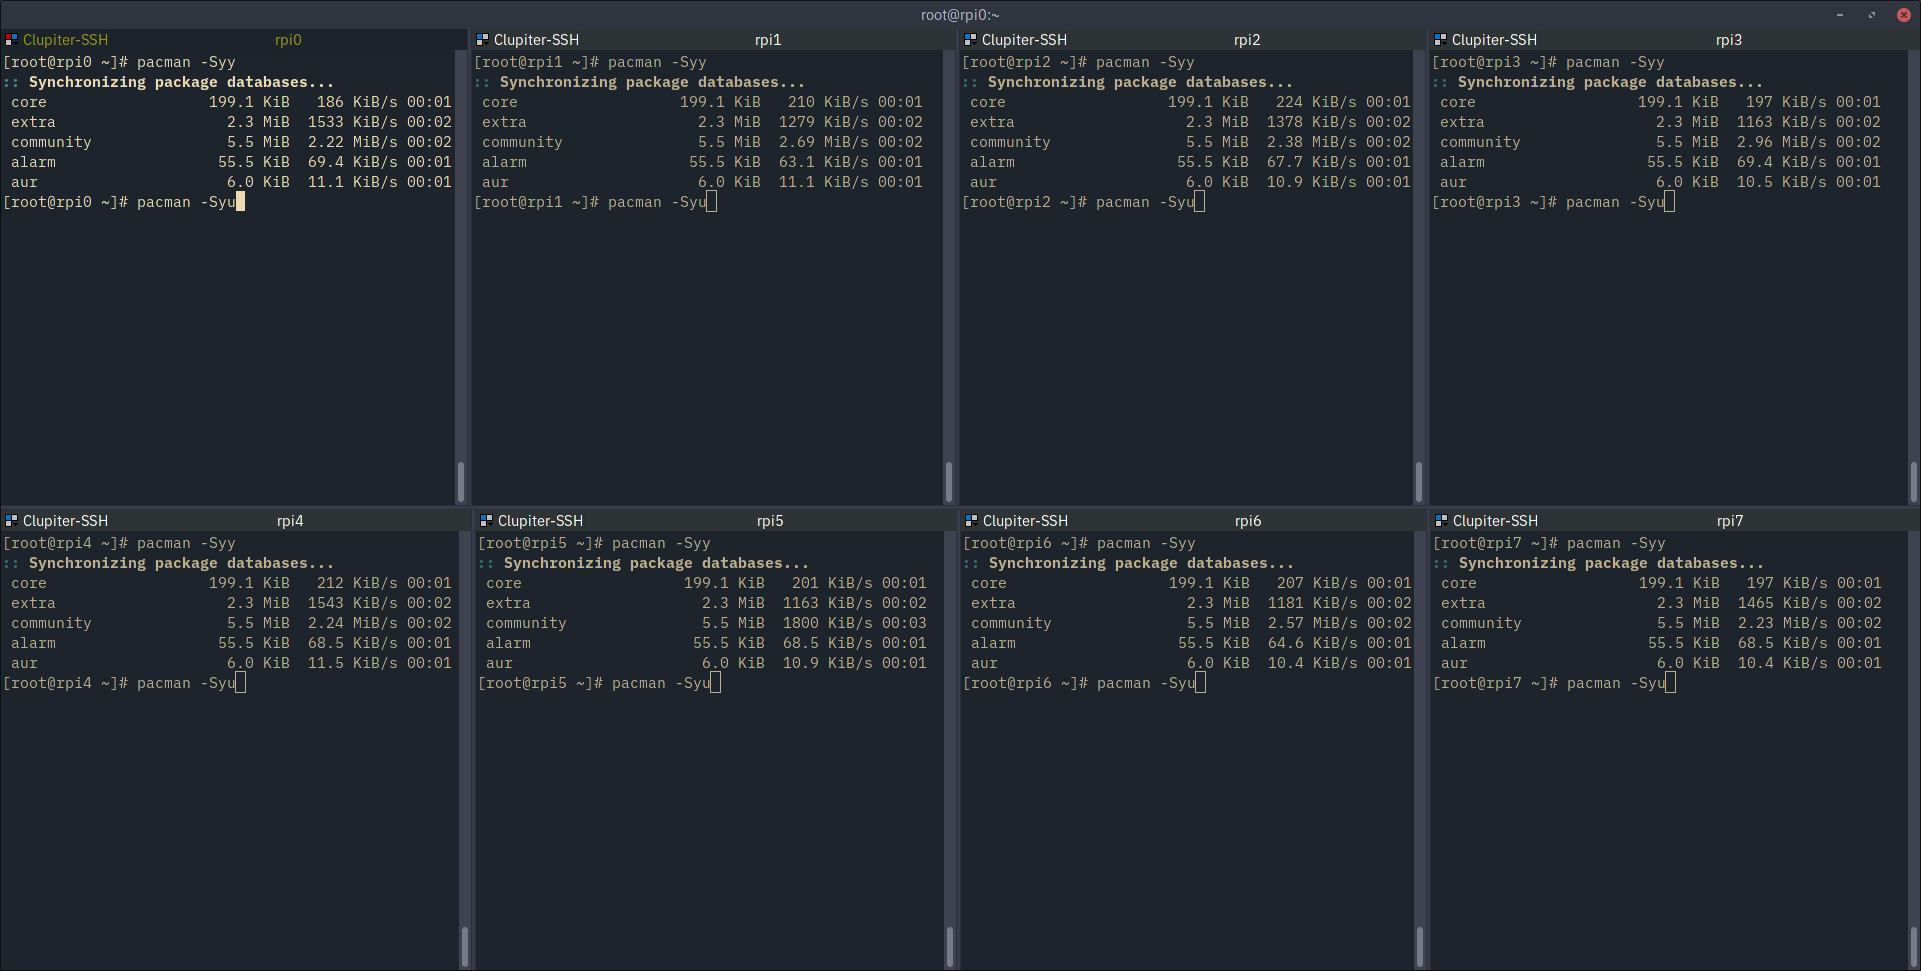
\includegraphics[width=\textwidth]{img/terminator_update.png}
  \caption{Operación en paralelo de Clúpiter con terminator}
  \label{fig:terminator_update}
\end{figure}

\printglossary[type=\acronymtype,title=\nomeglosarioacronimos]
\printglossary[title=\nomeglosariotermos]

\bibliographystyle{IEEEtranN}
\bibliography{\bibconfig,bibliografia/bibliografia}
\cleardoublepage

\end{document}

%%%%%%%%%%%%%%%%%%%%%%%%%%%%%%%%%%%%%%%%%%%%%%%%%%%%%%%%%%%%%%%%%%%%%%%%%%%%%%%%
